% !TeX encoding = UTF-8
% !TeX program = xelatex
% !TeX spellcheck = en_US

%-----------------------------------------------------------------------
% 中国科学: 信息科学 中文模板, 请用 CCT-LaTeX 编译
% http://scis.scichina.com
% 四川师范大学图灵的猫注释:也可以在Overleaf中使用XeLaTeX直接编译,
% 例如:
%-----------------------------------------------------------------------

\documentclass{Sichuan Normal University}
%\usepackage{breakurl}
%\captionsetup[subfloat]{labelformat=simple,captionskip=0pt}

%%%%%%%%%%%%%%%%%%%%%%%%%%%%%%%%%%%%%%%%%%%%%%%%%%%%%%%
%%% 作者附加的定义
%%% 常用环境已经加载好, 不需要重复加载
%%%%%%%%%%%%%%%%%%%%%%%%%%%%%%%%%%%%%%%%%%%%%%%%%%%%%%%


%%%%%%%%%%%%%%%%%%%%%%%%%%%%%%%%%%%%%%%%%%%%%%%%%%%%%%%
%%% 开始
%%%%%%%%%%%%%%%%%%%%%%%%%%%%%%%%%%%%%%%%%%%%%%%%%%%%%%%

\begin{document}

%%%%%%%%%%%%%%%%%%%%%%%%%%%%%%%%%%%%%%%%%%%%%%%%%%%%%%%
%%% 作者不需要修改此处信息
\ArticleType{\href{https://github.com/mathliuyang/PINNuclear-Neutrons}{GitHub}}
%\SpecialTopic{}
%\Luntan{中国科学院学部\quad 科学与技术前沿论坛}
\Year{2023}
\Vol{50}
\No{1}
\BeginPage{1}
\DOI{}
\ReceiveDate{}
\ReviseDate{}
\AcceptDate{}
\OnlineDate{}
%%%%%%%%%%%%%%%%%%%%%%%%%%%%%%%%%%%%%%%%%%%%%%%%%%%%%%%

\title{PINNuclear-Neutrons 项目笔记}{PINNuclear-Neutrons}

\entitle{PINNuclear-Neutrons Project Notes}{PINNuclear-Neutrons}

\author[1]{刘洋}{{mathliuyang@163.com}}
% \author[1]{张鹤瀛}{}
% \author[2]{孙晨}{}
% \author[3]{作者4}{}

\enauthor[1]{Liu Yang}{{mathliuyang@163.com}}
% \enauthor[1]{Zhang Heying}{}
% \enauthor[2]{Sun Chen}{}
% \enauthor[3]{Ming XING}{}

\address[1]{四川师范大学数学科学学院, 四川 成都 610066}
% \address[2]{成都外国语实验学校, 四川 成都 610031}
% \address[3]{作者单位, 城市 000000}

\enaddress[1]{School of Mathematical Sciences, Sichuan Normal University, Chengdu {\rm 610068}, Sichuan}
% \enaddress[2]{Chengdu Experimental Foreign Language School, Chengdu {\rm 610031}, Sichuan}
% \enaddress[3]{Affiliation, City {\rm 000000}, Country}

% \Foundation{基金资助}
\Foundation{通信作者简介:刘洋(1997-),男,研究生,主要研究方向:偏微分方程与数学物理}%\\中图分类号: O29 $\quad$ 文献标志码: A $\quad$ 文章编号 : 202310006 }
\AuthorMark{mathliuyang}

% \AuthorCitation{作者1, 作者2, 作者3, 等}
% \enAuthorCitation{Xing M, Xing M M, Xing M, et al}

% \comment{\dag~同等贡献}
%\encomment{\dag~Equal contribution}

\abstract{PINNuclear-Neutrons项目的主要目标在于学习并复现刘东老师团队的核反应堆物理学论文,该论文通过物理反应神经网络(PINN)和深度学习技术解决多维中子学扩散方程,以实现对中子传输的精确模拟,为核能技术提供高效准确的数值求解方法.

在学习过程中,首先深入探讨了PINN和L-BFGS优化算法等核心知识,并系统性学习了核反应堆物理分析的基础知识,包括裂变能量释放、链式裂变反应、热中子反应堆中子循环等,为后续中子学扩散方程的学习奠定了基础.

对刘东老师的论文《基于PINN深度机器学习技术求解多维中子学扩散方程》的深入研读中,全面总结了其中提及的中子学扩散方程模型以及PINN的应用.特别关注了论文提出的特征值方程加速收敛方法、$k_{\text{eff}}$高效并行搜索方法、样本网格点不均匀分布策略等关键技术,并通过数值验证程序的复现验证了这些方法在不同条件下的有效性.

在实际算法程序的复现实践中,通过深度机器学习的超参数设置和临界条件下稳态扩散方程的验证,解决了一系列问题,同时也发现了一些理论上的疑虑.尽管项目中仍存在理解上的挑战,但这一过程为对PINN和深度学习在核反应堆物理中子学领域应用的深刻认识提供了支持.

未来,将进一步深入探讨并拓展这一方法在反应堆物理中子学领域的应用,同时期待将其应用于更广泛的工程实际问题.通过学习这篇论文,对深度学习技术在解决科学与工程问题中的潜力有了更为清晰的认识,为进一步的学术研究提供了新的思路和启示.}

\enabstract{The primary objective of the PINNuclear-Neutrons project is to study and replicate the research conducted by Professor Liu Dong's team in the field of nuclear reactor physics. Their paper explores the application of Physics-Informed Neural Networks (PINN) and deep learning techniques to solve the multi-dimensional neutron diffusion equations. The project aims to achieve accurate simulation of neutron transport, providing an efficient and precise numerical solution for nuclear energy applications.
During the learning process, a comprehensive exploration of core concepts such as PINN and the L-BFGS optimization algorithm was undertaken. Foundational knowledge in nuclear reactor physics analysis was systematically acquired, encompassing fundamental concepts like fission energy release, chain reaction fission, and neutron circulation in thermal neutron reactors, laying the groundwork for subsequent studies on neutron diffusion equations.
In the in-depth review of Professor Liu Dong's paper titled "Solving Multi-dimensional Neutron Diffusion Equations using PINN Deep Machine Learning Technology," a thorough summary of the neutron diffusion equation models and the application of PINN was provided. Special attention was given to key techniques proposed in the paper, including the acceleration method for eigenvalue convergence, efficient parallel search for $k_{\text{eff}}$, and strategies for uneven distribution of sample grid points. These techniques were validated through the reproduction of numerical verification procedures under different conditions, confirming their effectiveness.
In the practical implementation of the algorithm, challenges were addressed through the fine-tuning of hyperparameters in deep machine learning and the validation of steady-state diffusion equations under critical conditions. While certain theoretical ambiguities persisted throughout the project, the process significantly contributed to a profound understanding of the application of PINN and deep learning in the domain of neutron physics in nuclear reactors.
Looking ahead, there is a commitment to further explore and expand the application of this methodology in the field of neutron physics in reactor physics. Simultaneously, there is an anticipation of its application to a broader spectrum of engineering challenges. Through the study of this paper, a clearer understanding of the immense potential of deep learning techniques in addressing scientific and engineering problems has emerged, providing novel perspectives and insights for future academic research.}

\keywords{基于物理信息指引的神经网络模型; 深度学习; 核反应堆; 中子学扩散方程}

\enkeywords{PINN; Deep Learning; Nuclear Reactor; Neutron Diffusion Equation}

\maketitle
\newpage
\tableofcontents  % 生成目录
\clearpage % 使用\clearpage分页,使图表索引独立于文档目录

\listoffigures % 生成图表索引

\newpage
\section*{引言}
随着人工智能技术的迅猛发展,深度学习神经网络(DNNs)在解决复杂偏微分方程(PDE)的领域引起了广泛的兴趣.在核反应堆设计和工程领域,中子学扩散模型是核反应堆工程设计的重要组成部分.传统的中子扩散模型采用有限差分法(FDM)和有限元法(FEM)等数值方法进行求解,这些方法在工程实践中取得了显著的成功.
然而,随着深度学习技术的不断发展,一种新的方法已经崭露头角,即基于物理信息指导的神经网络模型(PINN),它在解决微分方程方面展现出巨大潜力.DNNs首次用于解微分方程是在1998年由Lagaris提出的\cite{lagarisArtificialNeuralNetworks1998},后来由Raissi和Karniadakis进一步发展成为基于物理信息的神经网络(PINNs)\cite{raissiPhysicsinformedNeuralNetworks2019},
将方程和边界条件等物理信息的知识作为损失函数引入到神经网络训练当中,通过这种方法将问题的物理信息考虑进去,不再仅仅依靠数据驱动的方法来使得网络拟合偏微分方程的解函数;同时,此研究也指出如果将方程中的系数当作未知参数也可以完成发现方程的任务.此后,便有许多研究围绕基于物理信息的神经网络展开,而这些研究通常可以总结为调整神经网络结构,更改损失函数的形式,挑选不同的激活函数,采用不同的优化策略.
PINN模型充分利用了深度学习神经网络的通用逼近能力,同时能够处理多维高阶复杂微分方程.与传统数值方法相比,PINNs具有多方面的优势,包括无需事先收集大量训练数据、适用于正向和反向问题、无空间几何限制等.因此,PINNs已经引起了广泛的研究兴趣,并在热传递、结构动力学、流体力学、固体力学以及核反应堆动力学等多个领域取得了重要突破.

本PINNuclear-Neutrons项目笔记旨在深入理解PINN模型的原理和应用,通过推导和复现刘东老师的研究工作\cite{LiuDongJiYuPINNShenDuJiQiXueXiJiShuQiuJieDuoWeiZhongZiXueKuoSanFangCheng2022},进一步探讨PINN模型在核反应堆设计和工程中的潜在应用.将重点关注PINN模型的工作原理、关键参数的影响以及可能的优化方向,以便更好地理解和应用这一创新方法.通过本学习笔记,希望能够为核反应堆设计和工程领域的研究人员提供有关PINNs的深入见解,以应对复杂问题和挑战.

\section{预备知识:PINN 相关理论和技术}
本章的主要内容是介绍相关理论和技术,首先介绍基于物理信息的神经网络,通过这种方法可以将物理信息引入到神经网络当中,然后介绍了本文方法中所用到的二阶优化函数 L-BFGS,为了网络更快更好的优化.最后介绍了核反应堆物理的相关知识,为后文的方法介绍做好理论上的准备.
\subsection{基于物理信息的神经网络}
使用神经网络逼近函数从万能逼近定理被提出之后就一直是科学计算的重要方向,然而随着数据时代的到来,大数据在人工智能领域取得了巨大的成功,于是人们想通过数据驱动的方式来拟合函数,
但对于某些难以求解的函数,函数的解析解和数值解很难获得,无法大量产生训练神经网络所需要的数据.并且数据驱动的方法还会降低模型的泛用性,只在有监督的点的位置能达到对应的精度,
而在做推断位置的点所求出的值精度就会与训练时相差很多,直至采点够密集才能使求解精度达到对应要求.

为此 Raissi 等人在 2019 年提出了基于物理信息的神经网络(PINN)\cite{raissiPhysicsinformedNeuralNetworks2019},通过将物理方程条件作为损失函数,将物理方程信息参与到神经网络的训练过程之中.
当网络训练时,神经网络迭代优化所反向传播的不仅仅有数值上的损失,同时还有物理方程的损失,这样就可以对神经网络所表示的空间进行限制,逐渐去逼近真正的解空间.
而且有了物理信息的引入,网络对数据的要求也逐渐降低,不再完全依赖数据驱动,在有很少的数据,甚至没有数据的情况下依然能的到很好的回归效果,大大增加了网络的泛用性和稳定性.
具体神经网络结构如下图 \ref{fig:PINN Network Structure} 所示.
\begin{figure}[H]
    \centering
    \includegraphics[width=0.8\textwidth]{./figure/PINN网络结构图.pdf}
    \cnenfigcaption{PINN网络结构图}{PINN Network Structure}
    \label{fig:PINN Network Structure}
    \end{figure}
如图中所示定义损失函数为:
\begin{equation}
    M S E=M S E_u+M S E_{B C, I C}+M S E_R
    \label{eq:损失函数}  
\end{equation}其中 $M S E_R$ 是解的数值约束, 只对能取到解的值的点进行约束, 通过数值约束来使得神经网络拟合对应的函数; $M S E_{B C, I C}$ 是初边值条件的约束, 当一个点来自于初边值中任意一个点时, 需要满足其对应的初边值条件, 通过边值条件来限制解空间; 
$M S E_u$ 是方程本身的约束, 对于内部区域的点, 都需要满足微分方程, 通过微分方程来限制解空间.当损失函数整体趋于零时, 可以认为神经网络很好的拟合了满足初边值条件和方程约束的解, 所以此时解方程问题变成了满足对应损失函数的优化问题, 可以使用神经网络的优化方法来求得对应方程的解.
% \subsubsection{PINN 求解反问题}

\subsection{L-BFGS 优化算法}
常用的人工智能优化算法如 $\mathrm{Adam}, \mathrm{SGD}$ 等都是在一阶梯度下降法 (Gradient Descent) 上改进的, 而 L-BFGS 是基于二阶优化算法牛顿法改进的.牛顿法作为二阶的优化算法收敛速度要远快于一阶算法的, 
但是牛顿法需要计算海森矩阵的逆矩阵, 运算成本很高, 所以针对这个问题, 人们提出了 BFGS 算法和 L-BFGS 算法降低内存的需求, 在介绍此算法前, 先介绍牛顿法的过程.

设 $f(x)$ 的零点为 $\tilde{x}$, 随机选取初始点 $x_0$, 做 $f(x)$ 的切线得到 $y=f\left(x_0\right)+$ $f^{\prime}\left(x_0\right)\left(x-x_0\right)$, 令 $y=0$, 得到 $x_1=x_0-\frac{f\left(x_0\right)}{f^{\prime}\left(x_0\right)}$, 
由此可以得到递推公式 $x_{\mathrm{n}+1}=$用目标函数 $f(x)$ 的二阶泰勒展开求驻点, 即 $f(x) \approx f\left(x_{\mathrm{n}}\right)+f^{\prime}\left(x_{\mathrm{n}}\right)\left(x-x_n\right)+$ $\frac{1}{2} f^{\prime \prime}\left(x_n\right)\left(x-x_n\right)^2$, 
对其进行求导可得 $f^{\prime}\left(x_{\mathrm{n}}\right)+f^{\prime \prime}\left(x_n\right)\left(x-x_n\right)=0$, 由此更新 $x$ 来得到是目标函数最小的点.

当 $f(x)$ 是多元函数时, $x$ 与 $f^{\prime}(x)$ 为向量, 记 $f^{\prime}(x)$ 为 $g, f^{\prime \prime}(x)$ 为海森矩阵记为 $H$,则牛顿法在多元情况下的迭代公式变为 $x_{k+1}=x_k-g_k H_k^{-1}, k=0,1, \cdots$, 其中 $H_k^{-1}$是海森矩阵的逆, 
而直接求海森矩阵的逆十分困难, 所以 BFGS 算法提出通过迭代来近似 $H_k^{-1}$, 即:
\begin{equation}
    B_{k+1}^{-1}=\left(I-\frac{\delta_k y_k^T}{y_k^T \delta_k}\right) B_k^{-1}\left(I-\frac{y_k \delta_k^T}{y_k^T \delta_k}\right)+\frac{\delta_k \delta_k^T}{y_k^T \delta_k}
\label{eq:BFGS}
\end{equation}其中 $B_{k+1}^{-1}$ 是对 $H_{k+1}^{-1}$ 的逼近, $B_0^{-1}=I, \delta_k=x_{k+1}-x_k, y_k=g_{k+1}-g_k$ .
利用 $B_k^{-1}$ 的迭代公式, 每次都需要储存 $B$, 当数据维度很大时, 对计算机的内存需求也变得很高, 于是 L-BFGS 方法提出只储存 $\delta_k$ 与 $y_k$, 每个 $B_k^{-1}$ 都可由 $\delta_{1, \cdots, k}$与 $y_{1, \cdots, k}$ 迭代计算得出, 但当 $\mathrm{k}$ 过于大时, 计算机内存仍然会面临内存不足的风险, 于是在算法中可以设定一个超参数 $\mathrm{N}$, 当 $\mathrm{k}$ 超过 $\mathrm{N}$ 时, 释放前 $k-N$ 项,仅用最近的 $\mathrm{N}$ 项来逼近 $B_k^{-1}$, 虽然会损失部分精度, 但可以在有限的内存条件下完成函数的优化.

L-BFGS 仍然面临一个问题, 就是当初始点与函数最优解的点相距过远时, L-BFGS 算法可能会收敛到鞍点, 所以在本文实际应用时会先用 Adam 优化算法寻找一个最优解可能存在的区域, 再使用 L-BFGS 优化方法加快收敛的速度, 得到更好的优化结果.

\section{预备知识:核反应堆物理分析}

核反应堆是一种能以可控方式实现自续链式核反应的装置.根据原子核产生能量的方式, 可以分为裂变反应堆和聚变反应堆两种\cite{XieZhongShengHeFanYingDuiWuLiFenXi2020}.当今世界上已建成和广泛使用的反应堆都是裂变反应堆, 聚变反应堆目前尚处于研究设计阶段.裂变反应堆通过把一个重核裂变为两个中等质量核而释放能量.它是由核燃料、冷却剂、慢化剂、结构材料和吸收剂等材料组成的一个复杂系统.按用途不同, 裂变反应堆可分为生产堆、实验堆和动力堆.按冷却剂或慢化剂的种类不同可分为轻水堆、重水堆、气冷堆和液态金属冷却快中子增殖堆.按引起裂变反应的中子能量不同,又可分为热中子反应堆和快中子反应堆.

\subsection{裂变能量的释放}

根据结合能公式可以算出, 实验上也已测出, ${ }^{235} \mathrm{U}$ 核一次裂变大约释放 $200 \mathrm{MeV}$ 的能量,
其中裂变碎片的动能约占总释放能量的 $80 \%$, 裂变能量的大致分配如表 \ref{tab:核裂变释放的能量} 所示.裂变能量的绝大部分都在堆内转变为热能.由于中微子不带电, 其质量几乎为零, 因而它几乎不与堆内任何物质作用.因此, 中微子所具有的 $12 \mathrm{MeV}$ 的能量, 是不能利用的.另一方面, 裂变中子将被堆内各种材料的核吸收而发生 $(\mathrm{n}, \gamma)$ 反应, 这要释放出 $3 \sim 12 \mathrm{MeV}$ 的能量.虽然这部分能量并不是核裂变时直接放出来的, 但它也是裂变带来的后果, 并且这部分能量的绝大部分也在堆内转变为热能, 故通常把这一部分能量也归人裂变能量.可利用的裂变能量中大约 $97 \%$分配在燃料内, 不到 $1 \%$ (为 $\gamma$ 射线能量) 在堆屏蔽层内, 其余能量则分配在冷却剂和结构材料内.确切地讲, 每次裂变可利用的能量因堆型的不同而不同, 一般计算时, 可以近似地认为 ${ }^{235} \mathrm{U}$ 核每次裂变可利用的能量约为 $200 \mathrm{MeV}$ .

\begin{table}[H]
    \caption{核裂变释放的能量}
    \label{tab:核裂变释放的能量}
    \centering
    \begin{tabular}{cc|cc}
        \toprule 
        能量形式 & 能量 $/ \mathrm{MeV}$ & 能量形式 & 能量 $/ \mathrm{MeV}$\\
        \midrule 
        裂变碎片的动能 & 168 & 裂变产物 $\gamma$ 衰变-缓发 $\gamma$ 能量 & 7\\
        裂变中子的动能 & 5 & 裂变产物 $\beta$ 衰变-缓发 $\beta$ 能量 & 8\\
        瞬发 $\gamma$ 能量 & 7 & 中微子能量 & 12\\
        \midrule
        \multicolumn{2}{c}{共计} & \multicolumn{2}{c}{207} \\
        \bottomrule
    \end{tabular}
\end{table}
    
应该指出, 裂变产物的衰变 $\beta$ 和 $\gamma$ 射线的能量约占总裂变能量的 $4 \% \sim 5 \%$, 它们是裂变碎片在衰变过程中发射出来的, 即这部分能量释放是有一段时间延迟的.因而停堆后, 仍然会有衰变热量产生, 仍需进行冷却和屏蔽.这种停堆后衰变余热的导出问题是反应堆安全研究中重要的问题之一.

\subsection{链式裂变反应}

核反应堆中的核裂变反应是一种自持续的链式反应.当中子与裂变物质作用而发生核裂变反应时,裂变物质的原子核通常分裂为两个中等质量数的核 (称为裂变碎片).与此同时, 还将平均地产生两个以上新的裂变中子, 并释放出蕴藏在原子核内部的核能.在适当的条件下, 这些裂变中子又会引起周围其它裂变同位素的裂变, 如此不断地继续下去.这种反应过程称为链式裂变反应, 其反应过程如下图 \ref{fig:链式裂变反应} 所示.
\begin{figure}[H]
    \centering
    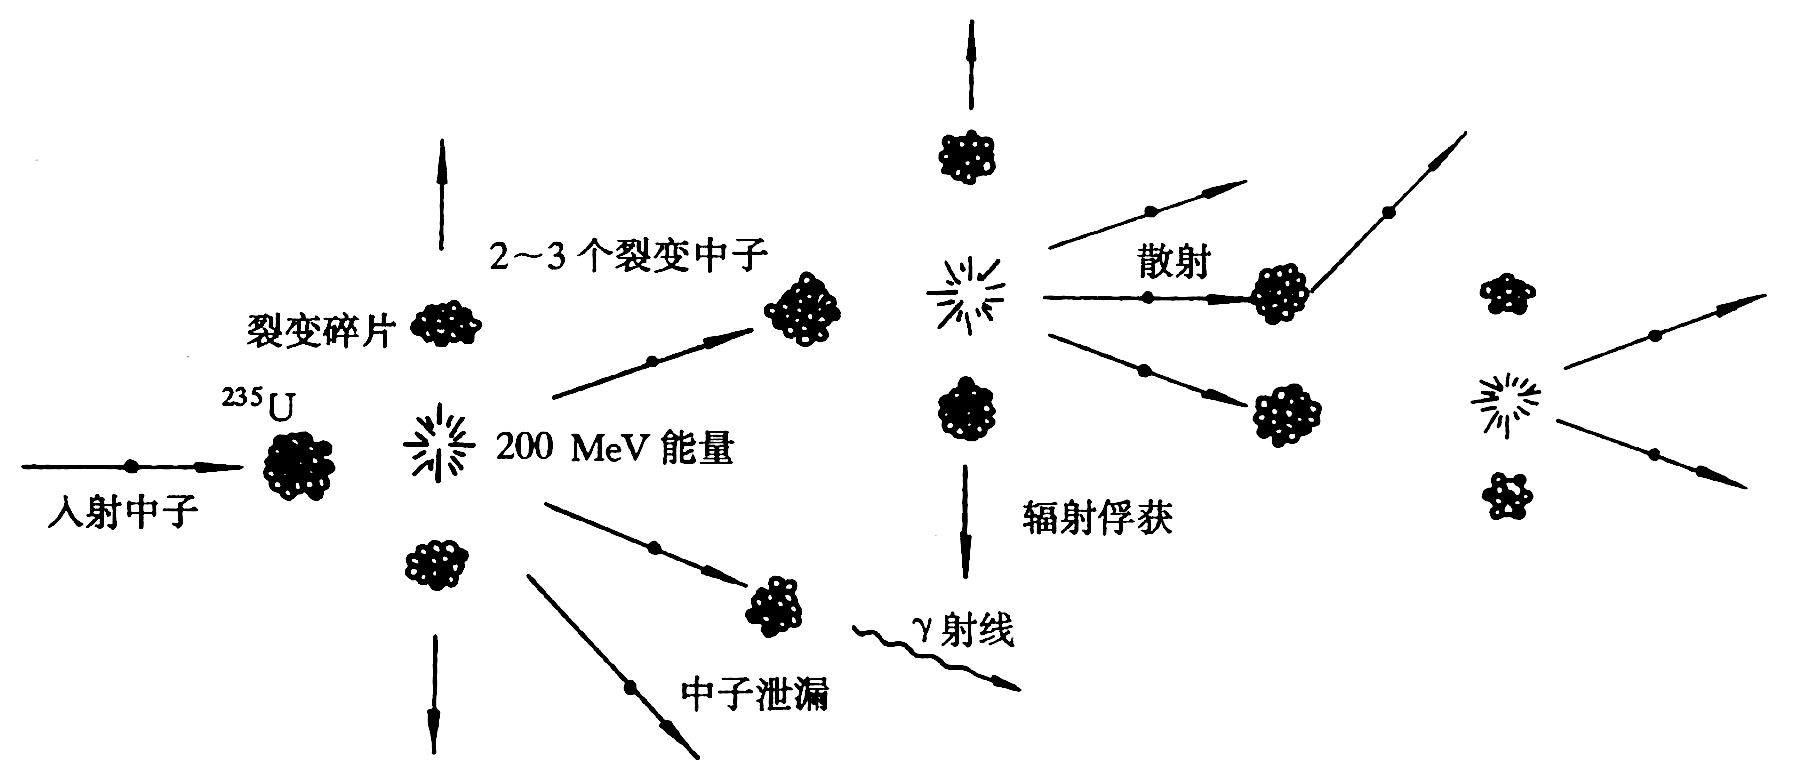
\includegraphics[width=0.8\textwidth]{./figure/链式裂变反应示意图.png}
    \cnenfigcaption{链式裂变反应示意图}{Chain fission reaction diagram}
    \label{fig:链式裂变反应}
    \end{figure}
如果每次裂变反应产生的中子数目大于引起核裂变所消耗的中子数目, 那么一旦在少数的原子核中引起了裂变反应之后, 就有可能不再依靠外界的作用而使裂变反应不断地进行下去.这样的裂变反应称作自续链式裂变反应.裂变核反应堆就是一种能以可控方式产生自续链式裂变反应的装置.它能够以一定的速率将蕴藏在原子核内部的核能释放出来.

从上面的讨论可以看出, 实现自续链式裂变反应的条件是: 当一个裂变核俘获一个中子产生裂变以后, 在新产生的中子中, 平均至少应该再有一个中子去引起另外一个核的裂变.由于
裂变物质每次裂变时平均地放出两个以上裂变中子, 因而实现自续的链式裂变反应是有可能的.但是, 因为核反应堆是由核燃料、慢化剂、冷却剂以及结构材料等所组成的装置, 所以在反应堆内, 不可避免地有一部分中子要被非裂变材料吸收.同时, 还有一部分中子要从反应堆中泄漏出去.因此, 在实际的反应堆中, 并不是全部的裂变中子都能引起新的核裂变反应.一个反应堆能否实现自续的链式裂变反应, 就取决于上述裂变、非裂变吸收和泄漏等过程中中子的产生率与消失率之间的平衡关系.如果在上述的反应过程中, 产生的中子数等于或多于消耗掉的中子数,则链式裂变反应将会自续地进行下去.

反应堆内自续链式裂变反应的条件可以很方便地用有效增殖系数 $k_{\mathrm{eff}}$ 来表示.它的定义是: 对给定系统, 新生一代的中子数和产生它的直属上一代中子数之比, 即
\begin{equation}
    k_{\mathrm{eff}}=\frac{\text { 新生一代中子数 }}{\text { 直属上一代中子数 }}
    \label{eq:有效增殖系数}
\end{equation}

上式的定义是直观地从中子的“寿命一循环”观点出发的.然而, 该式在实用上是不太方便的, 因为在实际问题中很难确定中子每 “代” 的起始和终了时间.例如, 在芯部中有的中子从裂变产生后立即就引起新的裂变, 有的中子则需要经过慢化过程成为热中子之后才引起裂变, 有的中子在慢化过程中便泄漏出系统或者被辐射俘获.所以, 实际上从中子的平衡关系来定义系统的有效增殖系数更为方便, 即
\begin{equation}
    k_{\text {eff }}=\frac{\text { 系统内中子的产生率 }}{\text { 系统内中子的总消失 (吸收 }+ \text { 泄漏) 率 }}
    \label{eq:有效增殖系数2}
\end{equation}

若芯部的有效增殖系数 $k_{\mathrm{eff}}$ 恰好等于 1 , 则系统内中子的产生率便恰好等于中子的消失率.这样, 在系统内已经进行的链式裂变反应, 将以恒定的速率不断地进行下去, 也就是说, 链式裂变反应过程处于稳态状况, 这种系统称为临界系统.若有效增殖系数 $k_{\mathrm{eff}}$ 小于 1 , 这时系统内的中子数目将随时间而不断地衰减, 链式裂变反应是非自续的, 这种系统便称为次临界系统.若有效增殖系数 $k_{\mathrm{efi}}$ 大于 1 , 则系统内的中子数目将随时间而不断地增加, 称这种系统为超临界系统.

显然, 有效增殖系数 $k_{\mathrm{eff}}$ 与系统的材料成分和结构 (例如易裂变同位素的富集度, 燃料-慢化剂的比例等)有关.同时, 它还与中子的泄漏程度, 或反应堆的大小有关.当反应堆的尺寸为无限大时, 中子的泄漏损失便等于零, 这时增殖系数将只与系统的材料成分和结构有关.通常, 把无限大介质的增殖系数称为无限介质增殖系数, 以 $k_{\infty}$ 表示.

对于实际的有限大小的反应堆, 中子的泄漏损失总是不可避免的.假定中子的不泄漏概率为 $\Lambda$, 它的定义是
\begin{equation}
    \Lambda=\frac{\text { 系统内中子的吸收率 }}{\text { 系统内中子的泄漏率 }}
    \label{eq:不泄漏概率}
\end{equation}

不泄漏概率 $\Lambda$ 主要取决于反应堆芯部的大小和几何形状, 当然它也和芯部成分有关.一般说来, 芯部愈大, 不泄漏概率也愈大.于是, 由式 \eqref{eq:有效增殖系数2} 和式 \eqref{eq:不泄漏概率} 可知, 有限尺寸芯部的有效增殖系数为
\begin{equation}
    k_{\text {eff }}=k_{\infty} \Lambda
    \label{eq:有效增殖系数3}
\end{equation}

当系统为无限大时, $\Lambda=1$, 这时有效增殖系数 $k_{\mathrm{eff}}=k_{\infty}$ .
根据以上的讨论, 立即可以得出反应堆维持自续链式裂变反应的条件是
\begin{equation}
    k_{\text {eff }}=k_{\infty} \Lambda=1
    \label{eq:反应堆维持自续链式裂变反应的条件}
\end{equation}

式 \eqref{eq:反应堆维持自续链式裂变反应的条件} 称为反应堆的临界条件.可以看出, 要使有限大小反应堆维持临界状态, 首先必须要求 $k_{\infty}>1$ .如果对于由特定的材料组成和布置的系统, 它的无限介质增殖系数 $k_{\infty}>1$, 那么, 对于这种系统必定可以通过改变反应堆芯部的大小, 找到一个合适的芯部尺寸, 恰好使 $k_{\infty} \Lambda=1$, 亦就是使反应堆处于临界状态, 这时反应堆芯部的大小称为临界大小.在临界情况下, 反应堆内所装载的燃料质量叫作临界质量.

反应堆的临界大小取决于反应堆的材料组成与几何形状.例如, 对于采用富集铀的反应堆, 它的 $k_{\infty}$ 比较大, 所以即使其不泄漏概率小一点, 仍然可能满足 $k_{\infty} \Lambda=1$ 的条件.这样, 用富集铀做燃料的反应堆, 其临界大小必定小于用天然铀做燃料的反应堆.决定临界大小的另一个因素是反应堆的几何形状.由于中子总是通过反应堆的表面泄漏出去, 而中子的产生则发生在反应堆的整个体积中, 因而, 要减少中子的泄漏损失, 增加不泄漏概率, 就需要减少反应堆的表面积与体积之比.在体积相同的所有几何形状中, 球形的表面积最小, 亦即球形反应堆的中子泄漏损失最小.然而, 实际中出于工程上的考虑, 动力反应堆是做成圆柱形的.
\subsection{热中子反应堆内的中子循环}
为了讨论反应堆内中子产生和消亡之间的平衡关系, 人为地将中子分成一代一代来处理是有益的.热中子反应堆内每代中子循环, 可以近似地用图 \ref{fig:热中子反应堆内的中子平衡} 表示.下面将对这一循环过程作进一步讨论.从以上的讨论可以知道, 反应堆内中子数目的增减与平衡, 主要取决于下列几个过程.

%%% 图文并排
\begin{wrapfigure}{r}{0.3\textwidth}
    \centering
    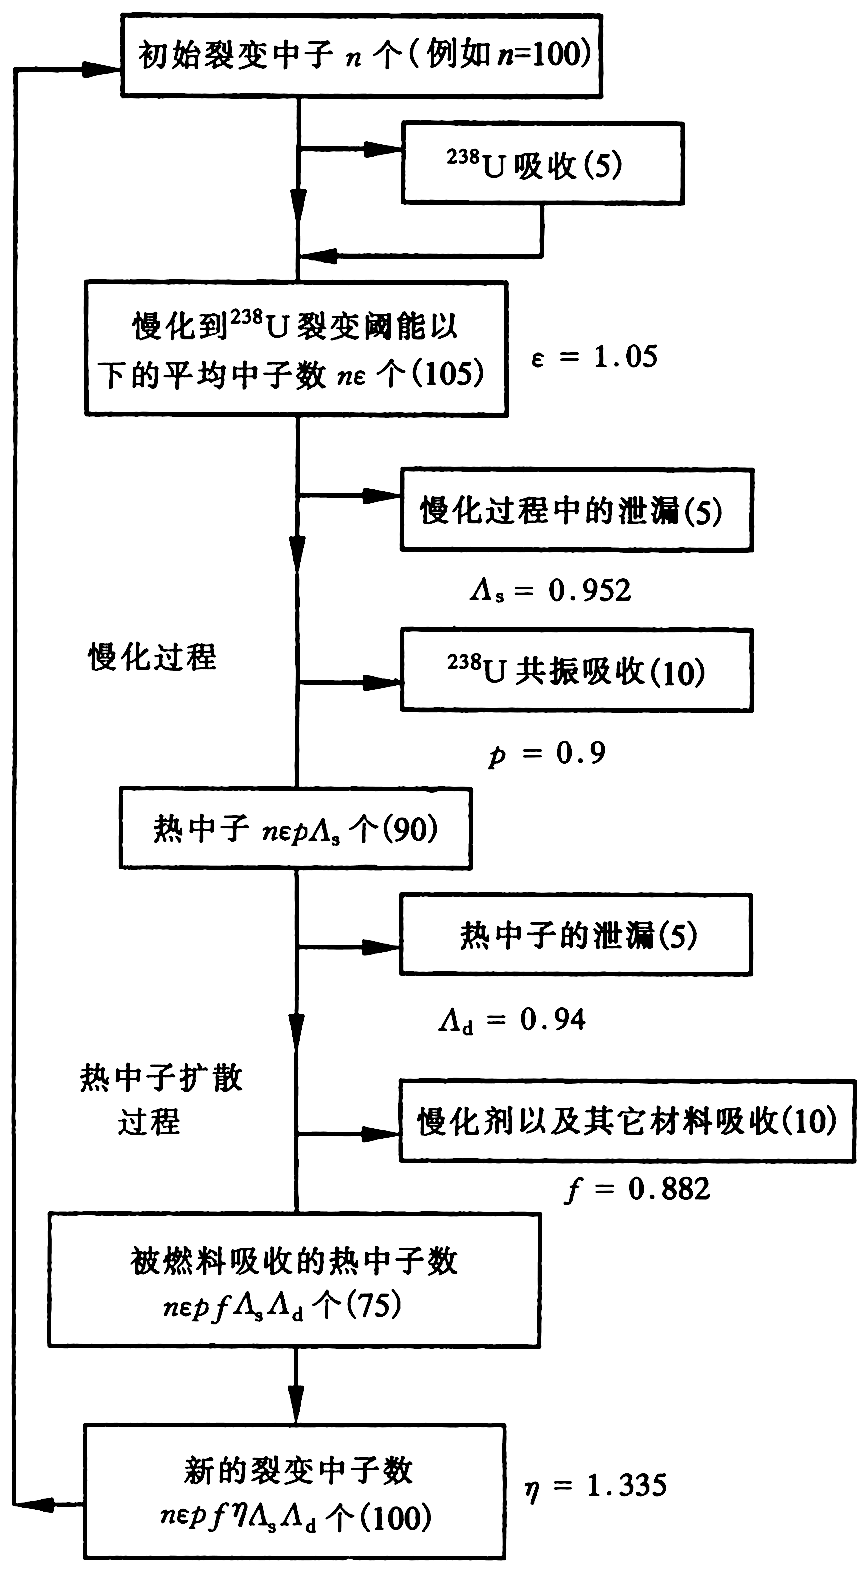
\includegraphics[width=0.3\textwidth]{./figure/热中子反应堆内的中子平衡.png} % 替换为你的图片文件名
    \cnenfigcaption{热中子反应堆内的中子平衡}{Neutron balance in thermal neutron reactor}
    \vspace{3mm}
    \label{fig:热中子反应堆内的中子平衡}
  \end{wrapfigure}
反应堆内中子数目的变化取决于上述 5 种过程竞争的结果.其中快中子增殖和燃料裂变将使反应堆内的中子数目增加, 其它过程使中子数目减少.为了定量计算, 就以上 5 个过程, 定义以下 5 个参量.

(1) ${ }^{238} \mathrm{U}$ 的快中子增殖.

(2) 慢化过程中的共振吸收.

(3) 慢化剂以及结构材料等物质的辐射俘获.

(4) 燃料吸收热中子引起的裂变.

(5)中子的泄漏.包括:慢化过程中的泄漏; 热中子扩散过程中的泄漏.

(1) 快中子增殖系数 $\varepsilon$ .它的定义: 由一个初始裂变中子所得到的、慢化到 ${ }^{238} \mathrm{U}$ 裂变阈能以下的平均中子数.由于初始裂变中子中, 大约有 $60 \%$ 的中子的能量在 ${ }^{238} \mathrm{U}$ 裂变阈能 (1. $1 \mathrm{MeV})$ 以上, 这些中子与 ${ }^{238} \mathrm{U}$ 核作用时, 有一部分能引起 ${ }^{238} \mathrm{U}$ 裂变而产生快中子, 这一过程称为 ${ }^{238} \mathrm{U}$ 的快中子增殖效应.

(2) 逃脱共振俘获概率 $p$ .裂变产生的快中子的平均能量为 $2 \mathrm{MeV}$, 在它们慢化的过程中, 要经过共振能区 $\left(1 \sim 10^4 \mathrm{eV}\right.$ ), 而 ${ }^{238} \mathrm{U}$ 核在该能区有许多共振峰(见图 \ref{fig:热中子反应堆内的中子平衡} ).因而在慢化中, 裂变产生的快中子中必然有一部分被 ${ }^{238} \mathrm{U}$ 核共振吸收而损失掉, 只有一部分快中子慢化至热中子.在慢化过程中逃脱共振吸收的中子份额就称为逃脱共振俘获概率, 用 $p$ 表示.

(3) 热中子利用系数 $f$ .它表示被燃料吸收的热中子数占被芯部中所有物质 (包括燃料在内) 吸收的热中子总数的份额. $f$ 定义为
\begin{equation}
    f=\text { 燃料吸收的热中子数 }
\end{equation}
这里分母中包括被燃料、慢化剂、冷却剂和结构材料等所有物质吸收的热中子总数.
对于均匀堆, 由于各种材料内的热中子通量密度相等, 因而
\begin{equation}
    f=\frac{N_{\mathrm{f}} \sigma_{\mathrm{a}, \mathrm{f}}}{N_{\mathrm{f}} \sigma_{\mathrm{a}, \mathrm{f}}+N_{\mathrm{m}} \sigma_{\mathrm{a}, \mathrm{m}}+N_{\mathrm{c}} \sigma_{\mathrm{a}, \mathrm{c}}+N_{\mathrm{s}} \sigma_{\mathrm{a}, \mathrm{s}}}
\end{equation}
其中,$N_{\mathrm{f}} 、 N_{\mathrm{m}} 、 N_{\mathrm{c}}$ 和 $N_{\mathrm{s}}$ 分别为在均匀混合物单位体积中燃料、慢化剂、冷却剂和结构材料的核子数.

(4) 有效裂变中子数 $\eta$ .它的定义: 核燃料每吸收一个热中子所产生的平均裂变中子数.设 $\Sigma_{\mathrm{a}}$ 和 $\Sigma_{\mathrm{f}}$ 分别为燃料的热中子宏观吸收截面和宏观裂变截面.由于燃料每吸收一个热中子引起裂变的概率为 $\Sigma_{\mathrm{f}} / \Sigma_{\mathrm{a}}$, 若设每次裂变所产生的平均裂变中子数为 $\nu$, 则显然有
\begin{equation}
\eta=\frac{\Sigma_{\mathrm{f}}}{\Sigma_{\mathrm{a}}} \nu
\end{equation}

(5) 不泄漏概率 $\Lambda$ .它是中子在慢化过程和热中子在扩散过程中不泄漏概率的乘积, 为
\begin{equation}
\Lambda=\Lambda_{\mathrm{s}} \Lambda_{\mathrm{d}}
\end{equation}
其中,$\Lambda_{\mathrm{s}}$ 为慢化过程中的不泄漏概率; $\Lambda_{\mathrm{d}}$为热中子扩散过程中的不泄漏概率.

定义了以上这些量以后, 便可以进一步定量地来研究热中子反应堆内中子的平衡过程.假设在某一代开始时有 $n$个裂变中子, 由于 ${ }^{238} \mathrm{U}$ 快中子增殖的结果, 中子数目将增加到 $n \varepsilon$ 个.这些中子继续慢化, 但是由于共振吸收将损失一部分中子, 所以只有 $n \varepsilon p$ 个中子能够逃脱共振吸收而慢化成热中子.如果考虑到中子的泄漏损失, 
那么, 实际上被吸收的热中子数目将只有 $n \varepsilon p \Lambda_{\mathrm{s}} \Lambda_{\mathrm{d}}$ 个.显然, 其中被燃料所吸收的热中子数目等于 $n \varepsilon p f \Lambda_{\mathrm{s}} \Lambda_{\mathrm{d}}$个, 其余部分的热中子被其它材料所吸收.被燃料吸收的热中子将使燃料发生核裂变反应, 而又重新放出新的裂变中子.
由于燃料每吸收一个热中子将产生 $\eta$个裂变中子, 因而新的裂变中子数目等于 $n \varepsilon p f \eta \Lambda_{\mathrm{s}} \Lambda_{\mathrm{d}}$ .作为一个例子, 在图 \ref{fig:热中子反应堆内的中子平衡} 中给出了各个过程的具体数值, 以便读者有定量的概念.
根据有效增殖系数的定义, 便可得出
\begin{equation}
k_{\text {eff }}=\frac{n \varepsilon p f \eta \Lambda_{\mathrm{s}} \Lambda_{\mathrm{d}}}{n}=k_{\infty} \Lambda
\end{equation}
其中,$\Lambda=\Lambda_{\mathrm{s}} \Lambda_{\mathrm{d}}$ .若根据图 \ref{fig:热中子反应堆内的中子平衡} 中给出的数值, 则 $\Lambda=0.8987$ .
由式 \eqref{eq:有效增殖系数3} 可以看出

\begin{equation}
k_{\infty}=\varepsilon p f \eta
\label{eq:四因子公式}
\end{equation}

式 \eqref{eq:四因子公式} 称为四因子公式.以上对热中子反应堆内中子平衡的分析方法称为“四因子模型”.在早期反应堆物理分析和计算中, 它曾被广泛地应用.同时, 它对热中子反应堆内中子的循环过程可以给出清晰的物理概念和形象的图形.但是它仅仅是对充分热化的热中子反应堆内的物理过程的一种近似的、简单的描述, 它并不能严格地描述一些更为复杂的反应堆内的物理过程.
目前, 伴随着对核反应堆物理过程的深人了解, 同时也随着计算机的发展, 它已被更为精确的建立在中子输运理论基础上的多群模型所代替, 而直接用数值方法求解分群扩散或中子输运方程.尽管如此, 在反应堆物理中无限介质增殖系数 $k_{\infty}$ 仍然是一个经常被用到的重要概念参数.
  
% \begin{figure}[H]
%     \centering
%     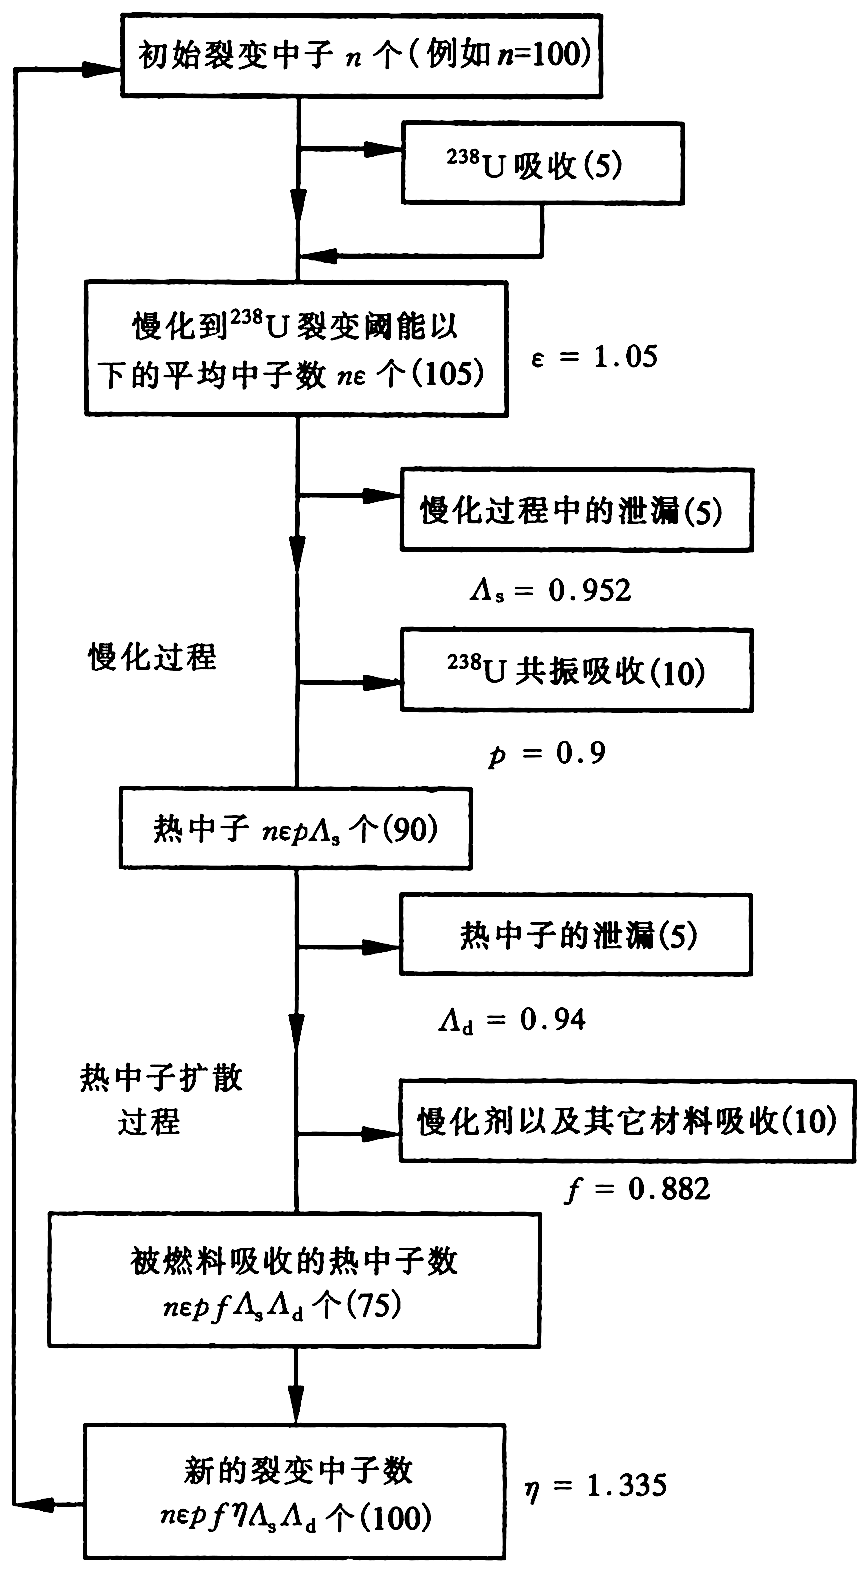
\includegraphics[width=0.5\textwidth]{./figure/热中子反应堆内的中子平衡.png}
%     \cnenfigcaption{热中子反应堆内的中子平衡}{Neutron balance in thermal neutron reactor}
%     \label{fig:热中子反应堆内的中子平衡}
%     \end{figure}

\subsection{单能中子扩散方程}
在物理学中, 已熟悉分子的扩散现象, 即分子间的无规则碰撞运动.分子从浓度大的地方向浓度小的地方扩散, 并且分子扩散的速率与分子密度的梯度成正比, 也就是服从分子扩散现象中的 “菲克扩散定律”.同样地, 若把一个中子源 (例如 $\mathrm{Ra}-\mathrm{Be}$ 源) 放到某一介质内, 可以通过测量仪器观察到, 中子不断地从源点扩散开来, 经过一段时间后, 介质内到处都有中子了.由于中子密度 (在热中子反应堆内约为 $10^{16} \mathrm{~m}^{-3}$ 数量级) 比起介质的原子核密度 (一般约为 $10^{28} \mathrm{~m}^{-3}$ ) 要小得多, 因而它与分子扩散现象不同, 其主要差别在于分子扩散是由于分子间的相互碰撞引起的, 而中子的扩散主要是中子与介质原子核间的散射碰撞的结果, 中子之间的相互碰撞可以略去不计.在中子密度大的地方, 中子与原子核碰撞的次数就多, 而每次碰撞以后, 中子通常要改变运动方向离开碰撞中心, 因此与分子的扩散相似, 中子总
是从中子密度高的地方向密度低的地方扩散.下面即将证明,与分子扩散相类似, 中子的扩散也服从与分子扩散相类似的定律, 它是中子扩散近似模型的基础.

显然中子扩散问题属于统计问题, 因而可以像气体动力论一样, 把它发展成为一种处理大量中子运动的宏观理论.例如, 在气体分子或热的扩散中扩散物质有一种倾向,就是从分子密度大的区域向分子密度小的区域移动 (扩散).中子的行为也一样, 从中子密度大的区域向中子密度小的区域移动 (扩散).它的规律服从气体动力学中的扩散规律, 因此可以以某种扩散方程为基础来处理大量中子行为的 (扩散) 宏观理论.

在扩散宏观理论中, 中子密度 $n(\boldsymbol{r}, E)$ 是一个重要的参量, 它描述了中子群在介质内的分布情况.另外, 还有以下两个参量也是经常要用到的重要参数.

(1) $\phi(r, E)$ .如前所述它与中子在介质中的核反应率密切相关.

(2) $\boldsymbol{J}(\boldsymbol{r}, E)$ .它定义为中子的净流密度
\begin{equation}
    \boldsymbol{J}(\boldsymbol{r}, E)=\int_{4 \pi} \boldsymbol{\Omega} \boldsymbol{\Phi}(\boldsymbol{r}, \boldsymbol{\Omega}) \mathrm{d} \boldsymbol{\Omega}
    \label{eq:中子的净流密度}
\end{equation}

从物理上看, 它是由很多具有不同方向的微分中子束矢量合成的量, 表示该处中子的净流动情况, 因而它是一个矢量.设 $n$ 表示该点的法线方向,则
\begin{equation}
    J_n(\boldsymbol{r}, E)=\boldsymbol{J}(\boldsymbol{r}, E) \cdot \boldsymbol{n}
    \label{eq:中子的净流密度2}
\end{equation}
就表示每秒穿过该点的净中子数目 (净中子流).它表示中子在介质中的流动情况.

链式核反应堆理论用到的一个基本原理, 就是所谓的 “中子数守恒”或者“中子数平衡”, 即在一定的体积 $V$ 内, 中子总数对时间的变化率应等于该体积内中子的产生率减去该体积内中子的吸收率和泄漏率.如果 $n(\boldsymbol{r}, t)$ 是 $t$ 时刻在 $\boldsymbol{r}$ 处的中子密度, 则在 $V$ 内中子数守恒的方程可写成
\begin{equation}
    \frac{\mathrm{d}}{\mathrm{d} t} \int_V n(\boldsymbol{r}, t) \mathrm{d} V=\text { 产生率 }(S) \text { - 泄漏率 }(L) \text { - 吸收率 }(A)
    \label{eq:中子数守恒}
\end{equation}

中子扩散方程就是根据这一平衡原则建立的.
首先计算中子的泄漏率.
让观察空间 $\boldsymbol{r}$ 处的微体积元 $\mathrm{d} V$ .知道 $\boldsymbol{J}(\boldsymbol{r}, t) \cdot \boldsymbol{n}$ 等于在 $r$ 处中子通过垂直于外法线 $n$ 的单位面积的净流动率.如果取 $n$ 为体积 $V$ 的表面积 $\mathrm{d} S$ 上的外法线单位向量, 那么 $\boldsymbol{J}(\boldsymbol{r}, t) \cdot n \mathrm{~d} S$ 就等于中子通过表面积元 $\mathrm{d} S$ 向外的净流率, 于是中子从体积 $V$ 的整个表面泄漏出去的总速率为
\begin{equation}
    \text { 泄漏率 }=\int_S \boldsymbol{J}(\boldsymbol{r}, t) \cdot \boldsymbol{n} \mathrm{d} S
    \label{eq:泄漏率}
\end{equation}

应用高斯散度公式可以把面积分变换成体积分,于是
\begin{equation}
    \text { 泄漏率 }=\int_S \boldsymbol{J}(\boldsymbol{r}, t) \cdot \boldsymbol{n} \mathrm{d} S=\int_V \nabla \cdot \boldsymbol{J}(\boldsymbol{r}, t) \mathrm{d} V=\int_V \operatorname{div} \boldsymbol{J}(\boldsymbol{r}, t) \mathrm{d} V
    \label{eq:泄漏率2}
\end{equation}

设源分布函数以 $S(\boldsymbol{r}, t)$ 表示, 它等于 $t$ 时刻 $\boldsymbol{r}$ 处每秒、每单位体积由源放出的中子数.因此, 在 $V$ 内中子的产生率为
\begin{equation}
    \text { 产生率 }=\int_V S(\boldsymbol{r}, t) \mathrm{d} V
    \label{eq:产生率}
\end{equation}
在 $V$ 内中子的吸收率可以表示为
\begin{equation}
    \text { 吸收率 }=\int_V \sum_{\mathrm{a}} \phi(\boldsymbol{r}, t) \mathrm{d} V
    \label{eq:吸收率}
\end{equation}
于是式 \eqref{eq:中子数守恒} 可以写成
\begin{equation}
    \frac{\mathrm{d}}{\mathrm{d} t} \int_V n(\boldsymbol{r}, t) \mathrm{d} V=\int_V S(\boldsymbol{r}, t) \mathrm{d} V-\int_V \sum_{\mathrm{a}} \phi(\boldsymbol{r}, t) \mathrm{d} V-\int_V \operatorname{div} \boldsymbol{J}(\boldsymbol{r}, t) \mathrm{d} V
    \label{eq:中子数守恒2}
\end{equation}

由于所有积分都是在相同的积分体积内进行的, 所以方程 \eqref{eq:中子数守恒2} 两边被积函数必然相等, 即
\begin{equation}
    \frac{\partial n(\boldsymbol{r}, t)}{\partial t}=S(\boldsymbol{r}, t)-\Sigma_{\mathrm{a}} \phi(\boldsymbol{r}, t)-\operatorname{div} \boldsymbol{J}(\boldsymbol{r}, t)
    \label{eq:中子数守恒3}
\end{equation}

方程 \eqref{eq:中子数守恒3} 叫做连续方程, 它实际上表征单位体积 (或微元) 内的中子数的平衡关系, 在反应堆理论中具有极为重要的意义.

连续方程 \eqref{eq:中子数守恒3} 是具有普遍意义的, 但其中具有两个未知函数 $\phi(\boldsymbol{r}, t)$ 及 $\boldsymbol{J}(\boldsymbol{r}, t)$, 
因此无法求解这个方程.如果在求解之前能找出 $\phi(\boldsymbol{r}, t)$ 和 $\boldsymbol{J}(\boldsymbol{r}, t)$ 之间的关系, 将其代入式 \eqref{eq:中子数守恒3}, 这样将其变成只含一个, 例如 $\phi(\boldsymbol{r}, t)$ 的方程, 问题就解决了.
为此,考虑稳态情况,也就是中子通量密度不随时间变化时,同时假设以下条件成立:
    \begin{itemize}
        \item[] \hspace{1mm}(1) 介质是无限的、均匀的;
        \item[] \hspace{1mm}(2) 在实验室坐标系中,散射是各向同性的;
        \item[] \hspace{1mm}(3) 介质的吸收截面很小,即 $\Sigma_{\mathrm{a}} \ll \Sigma_{\mathrm{s}}$;
        \item[] \hspace{1mm}(4) 中子通量密度是随空间位置缓慢变化的函数.
    \end{itemize}
在这种情况下,可以得到以下定理:

\begin{theorem}[菲克定律]
    中子流密度 $\boldsymbol{J}$ 正比于负的中子通量密度梯度, 即
    \begin{equation}
    \boldsymbol{J}=-D \operatorname{grad} \phi
    \label{eq:菲克定律}
\end{equation}
    其中比例常数 $D=\frac{\lambda_{\mathrm{s}}}{3}$, 并称作扩散系数.
\end{theorem}

应该指出, 在上述定理的推导过程中, 曾经假设在实验室坐标系中中子散射是各向同性的, 实际上, 这一假设只有对于重核才近似成立, 在一般情况下, 这种假设是不正确的.由中子输运理论可以证明, 为了对散射的各向异性作适当的修正, 扩散系数中, 必须用输运平均自由程 $\lambda_{\mathrm{tr}}$ 来代替式中的散射平均自由程 $\lambda_{\mathrm{s}}$ .菲克定律中的扩散系数 $D$ 为
\begin{equation}
    D=\frac{\lambda_{\text {tr }}}{3}
    \label{eq:扩散系数}
\end{equation}
    $\lambda_{\mathrm{tr}}$ 为输运平均自由程, 它等于
\begin{equation}
    \lambda_{\mathrm{tr}}=\frac{\lambda_{\mathrm{s}}}{1-\bar{\mu}_0}
    \label{eq:输运平均自由程}
\end{equation}其中: $\bar{\mu}_0$ 是实验室系统内的平均散射角余弦\cite{XieZhongShengHeFanYingDuiWuLiFenXi2020}, $\bar{\mu}_0=\frac{2}{3 A}$.对于重核, $\bar{\mu}_0 \ll 1$, 则 $\lambda_{\mathrm{tr}}$便近似地等于 $\lambda_{\mathrm{s}}$ .
式 \eqref{eq:菲克定律} 表明: 任一处净中子流动的方向与中子通量密度分布的梯度的方向相反.因为 $\operatorname{grad} \phi$ 的方向指向 $\phi$ 的增加方向, 所以 $J$ 的方向指向 $\phi$ 减小最快的方向.


在求出中子流密度 $J(r, E)$ 和中子通量 $\phi$ 的关系后, 就可以从中子连续方程直接导出只含有中子通量 $\phi$ 的中子扩散方程.如前所述, 根据连续方程

\begin{equation}
    \frac{\partial n(\boldsymbol{r}, t)}{\partial t}=S(\boldsymbol{r}, t)-\Sigma_{\mathrm{a}} \phi(\boldsymbol{r}, t)-\operatorname{div} \boldsymbol{J}(\boldsymbol{r}, t)
\end{equation}

它实际上表征单位体积 (或微元) 内的中子数的平衡关系.其中方程的右端第三项表示泄漏项.根据菲克定律它可以写成
\begin{equation}
    \operatorname{div} \boldsymbol{J}(\boldsymbol{r}, t)=-\operatorname{div} D \operatorname{grad} \phi=D \nabla^2 \phi
    \label{eq:中子数守恒4}
\end{equation}
同时由于假定所有中子都具有相同的能量, 所以中子通量密度
\begin{equation}
\phi=n v
\end{equation}
方程变为
\begin{equation}
    D \nabla^2 \phi-\Sigma_{\mathrm{a}} \phi+S=\frac{1}{v} \frac{\partial \phi}{\partial t}
    \label{eq:单能中子扩散方程}
\end{equation}其中, $\nabla^2$ 是拉普拉斯算符.在反应堆计算常用的几种坐标系中, $\nabla^2$ 的表达式如下:
\begin{align}
    \text{直角坐标系} & \quad \nabla^2 = \frac{\partial^2}{\partial x^2} + \frac{\partial^2}{\partial y^2} + \frac{\partial^2}{\partial z^2} \\
    \text{柱坐标系} & \quad \nabla^2 = \frac{\partial^2}{\partial r^2} + \frac{1}{r} \frac{\partial}{\partial r} + \frac{1}{r^2} \frac{\partial^2}{\partial \theta^2} + \frac{\partial^2}{\partial z^2} \\
    \text{球坐标系} & \quad \nabla^2 = \frac{\partial^2}{\partial r^2} + \frac{2}{r} \frac{\partial}{\partial r} + \frac{1}{r^2} \frac{\partial^2}{\partial \theta^2} + \frac{1}{r^2} \cot \theta \frac{\partial}{\partial \theta} + \frac{1}{r^2 \sin^2 \theta} \frac{\partial^2}{\partial \varphi^2}
    \end{align}
    
方程 \eqref{eq:单能中子扩散方程} 称为单能中子扩散方程,它是借助中子扩散的菲克定律从中子数守恒的连续方程推导而得的,是反应堆理论中的一个基本方程,在反应堆理论中广泛应用并占有很重要的位置.
\begin{remark}
    在扩散理论中有两个重要的物理参数: 扩散系数 $D$ 和扩散长度 $L$ .它们是确定中子在介质内扩散过程的重要参数.根据定义, 扩散长度为
    \begin{equation}
L^2=\frac{D}{\Sigma_{\mathrm{a}}}=\frac{\lambda_{\mathrm{a}} \lambda_{\mathrm{tr}}}{3}
\label{eq:扩散长度与扩散系数}
\end{equation}
或
\begin{equation}
L^2=\frac{\lambda_{\mathrm{a}} \lambda_{\mathrm{s}}}{3\left(1-\bar{\mu}_0\right)}=\frac{1}{3 \Sigma_{\mathrm{a}} \Sigma_{\mathrm{s}}\left(1-\bar{\mu}_0\right)}
\label{eq:扩散长度与扩散系数的关系}
\end{equation}
这便是扩散长度的计算公式.对于混合物, 则式 \eqref{eq:扩散长度与扩散系数的关系} 中的 $\Sigma_{\mathrm{a}} 、 \Sigma_{\mathrm{s}}$ 和 $\bar{\mu}_0$ 等都是指混合物的
平均值.对于热中子, 式中的 $\Sigma_{\mathrm{a}}$ 和 $\Sigma_{\mathrm{s}}$ 应该是热中子能谱的平均值.
\end{remark}

\subsubsection{扩散方程边界条件}
扩散方程式 \eqref{eq:单能中子扩散方程} 是一个微分方程, 它适用于普遍情况, 在它的普遍解中将包含有任意的积分常数.为了确定这些积分常数的数值, 就要根据具体问题在普遍解上加一些限制条件,也就是问题本身的物理或几何特性所规定的边界条件.边界条件的数目应恰好足以确定方程有唯一解.

下面讨论求解扩散方程时经常用到的几种边界条件.
\begin{itemize} 
    \item 在扩散方程适用的范围内, 中子通量密度的数值必须是正的、有限的实数.

    \item 在两种不同扩散性质的介质交界面上, 垂直于分界面的中子流密度相等, 中子通量密度相等.

设有两种不同介质的分界面 (见图 \ref{fig:在两种介质分界面上的中子扩散}),在分界面上所有沿正 $x$ (或负 $x$ ) 方向穿过 $A$介质的中子数必定等于同一方向穿过 $B$ 介质的中子数 (因为在分界面上不能有中子的积累或消耗), 即

\begin{equation}
\left.J_x^{+}\right|_A=\left.J_x^{+}\right|_B
\label{eq:界面上的中子流密度相等1}
\end{equation}
和
\begin{equation}
\left.J_x^{-}\right|_A=\left.J_x^{-}\right|_B
\label{eq:界面上的中子流密度相等2}
\end{equation}
将 $J_x^{+}$及 $J_x^{-}$的表示式代入式 \eqref{eq:界面上的中子流密度相等1} 及式 \eqref{eq:界面上的中子流密度相等2}, 然后两式相减便可得到
\begin{equation}
\left.D_A \frac{\mathrm{d} \phi}{\mathrm{d} x}\right|_A=\left.D_B \frac{\mathrm{d} \phi}{\mathrm{d} x}\right|_B
\label{eq:界面上的中子流密度相等}
\end{equation}

若两式相加则有
\begin{equation}
\phi_A=\phi_B
\label{eq:界面上的中子通量密度相等}
\end{equation}

式  \eqref{eq:界面上的中子流密度相等} 及式 \eqref{eq:界面上的中子通量密度相等} 便是扩散方程在分界面上的边界条件.

\item 介质与真空交界的外表面上,根据物理上的要求, 自真空返回介质的中子流等于零 (见图 \ref{fig:应用输运理论和扩散理论的外推距离求得的扩散方程的解}), 即
\begin{equation}
\left.J_x^{-}\right|_{x=0}=0
\end{equation}

反应堆的外表面就属于这种情况.空气虽然不是真空, 但是, 由于单位体积内的分子数比非气体介质要小得多, 所以, 中子在空气中的平均自由程比在非气体介质中的平均自由程
要大得多, 因而可以把空气近似地当作真空来处理.由于中子不可能自真空中散射回到介质中来,所以在 $x=0$ 处沿负 $x$ 方向上的中子流等于零.有
\begin{equation}
\left.J_x^{-}\right|_{x=0}=\frac{\phi_0}{4}+\left.\frac{\lambda_{\text {tr }}}{6} \frac{\mathrm{d} \phi}{\mathrm{d} x}\right|_{x=0}=0
\end{equation}

或者写成
\begin{equation}
\left.\frac{\mathrm{d} \phi}{\mathrm{d} x}\right|_{x=0}=-\frac{3 \phi_0}{2 \lambda_{\mathrm{tr}}}
\label{eq:外表面上的中子流密度等于零}
\end{equation}

这个条件可以写成更方便的形式.如果假想从交界面处将中子通量密度的分布曲线按它在交界面处的斜率向真空作直线外推 (见图 \ref{fig:应用输运理论和扩散理论的外推距离求得的扩散方程的解} 中的虚线), 则在离开交界面某个距离 $d$处的位置上中子通量密度将等于零, 于是有
\begin{equation}
\left.\frac{\mathrm{d} \phi}{\mathrm{d} x}\right|_{x=0}=-\frac{\phi_0}{d}
\end{equation}

而根据式 \eqref{eq:外表面上的中子流密度等于零} 有
\begin{equation}
d=\frac{2}{3} \lambda_{\mathrm{tr}}
\end{equation}

这里, $d$ 称为直线外推距离.
应当指出, 上述的直线外推距离 $d$ 是从扩散理论求出的, 但是扩散理论在真空交界处附近不适用, 因而由此求出的 $d$ 也是不精确的.按照更精确的中子输运理论, 对于平面边界的情况, 可以求得 $d=0.7104 \lambda_{\mathrm{tr}}$, 以后在计算中, 将采用这一数值.严格地讲, 外推距离 $d$与表面曲率半径有关, 但对于曲率较小的表面, 近似地应用 $0.7104 \lambda_{\mathrm{tr}}$ 这一数值不会产生很大的误差.这样,自由外表面 (真空边界)的边界条件可以用更简单的形式表示:
在自由表面外推距离 $d$ 处, 中子通量密度等于零.
最后必须强调指出, 这个边界条件仅仅是为了简化扩散方程的求解而采取的一种数学处理方法, 并不是说在自由表面外, 中子通量密度的变化是真的按照直线外推的那样, 在外推边界上等于零.实际上, 在自由表面以外中子通量密度的分布是没有意义的.这种外推边界仅仅是一种假想的边界概念, 只是表示利用上述外推距离作为扩散方程的边界条件可以在许多情况下得出比较满意的近似结果, 如图 \ref{fig:应用输运理论和扩散理论的外推距离求得的扩散方程的解} 所示.从图中可以看到, 应用输运理论的外推距离求得扩散方程的解, 除靠近边界附近有偏差外, 其它部分与输运理论的严格解吻合良好.


%%% 并排图
%%% 可在文中使用图\ref{fig1}、图\ref{fig2}引用图编号
\begin{figure}[!t]
    \centering
    \begin{minipage}[c]{0.48\textwidth}
    \centering
    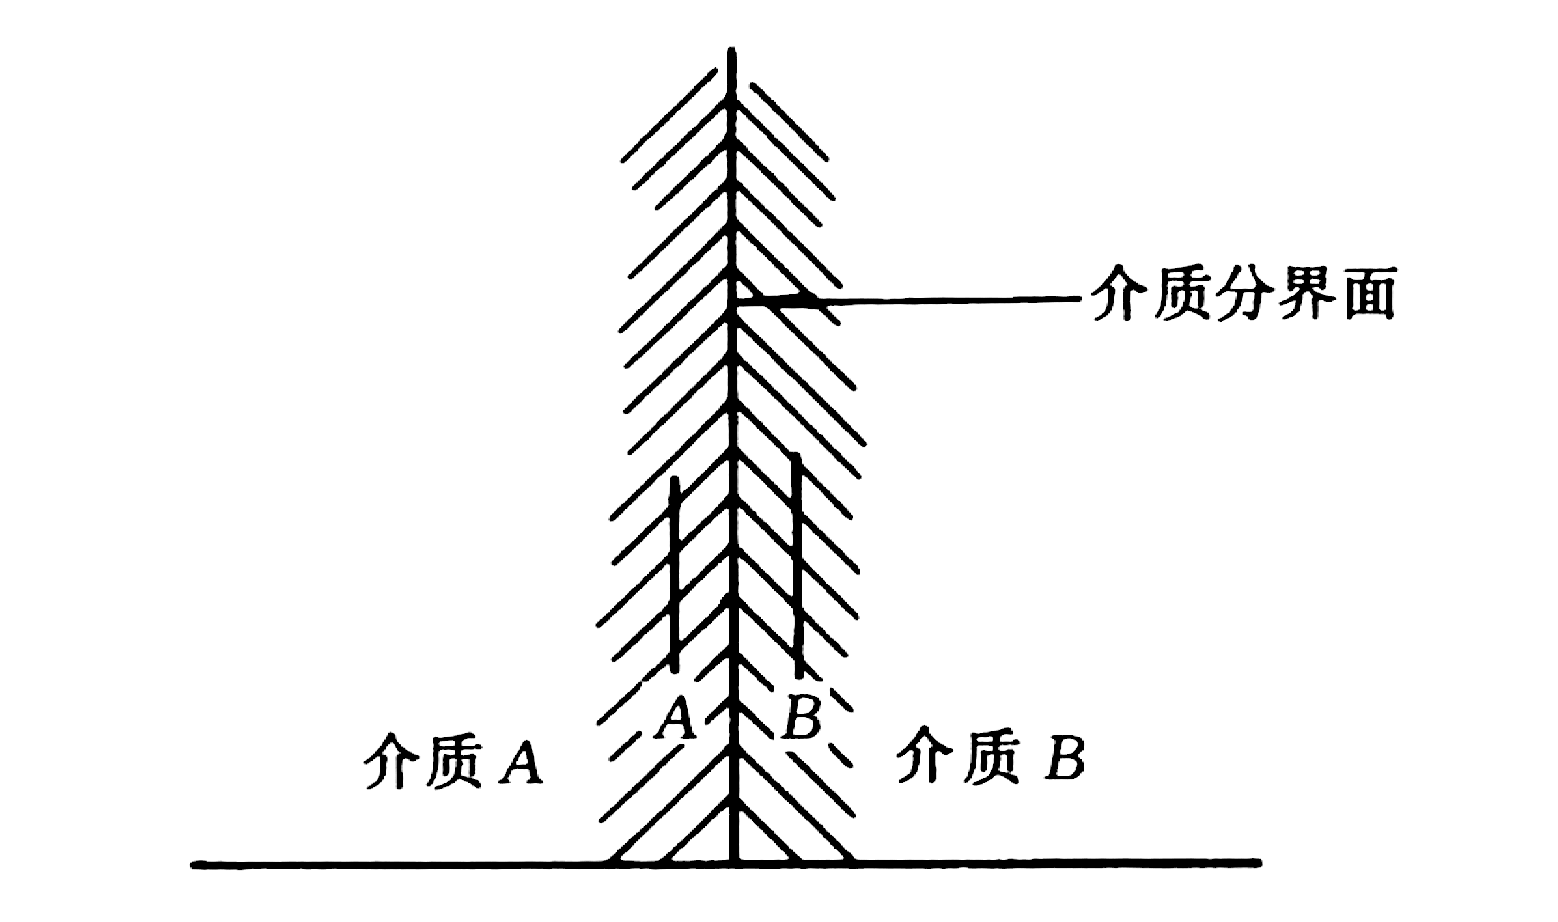
\includegraphics[width=0.8\textwidth]{./figure/在两种介质分界面上的中子扩散.png}
    \end{minipage}
    \hspace{0.02\textwidth}
    \begin{minipage}[c]{0.48\textwidth}
    \centering
    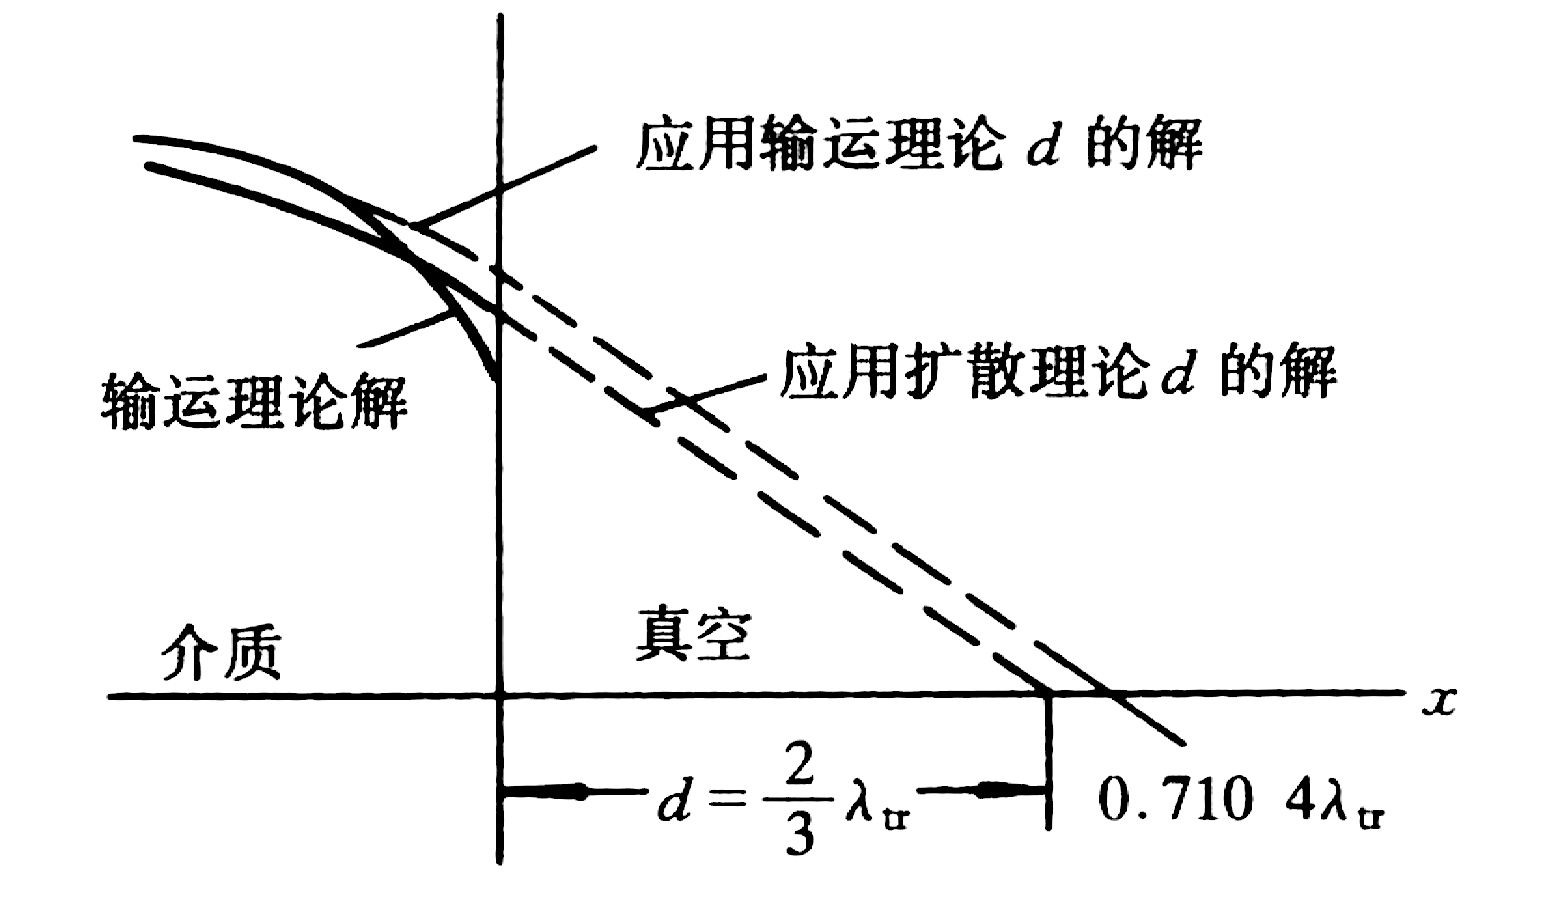
\includegraphics[width=0.8\textwidth]{./figure/应用输运理论和扩散理论的外推距离求得的扩散方程的解.png}
    \end{minipage}\\[3mm]
    \begin{minipage}[t]{0.48\textwidth}
    \centering
    \cnenfigcaption{在两种介质分界面上的中子扩散}{Neutron diffusion at the interface of two media}
    \label{fig:在两种介质分界面上的中子扩散}
    \end{minipage}
    \hspace{0.02\textwidth}
    \begin{minipage}[t]{0.48\textwidth}
    \centering
    \cnenfigcaption{外推距离求得的扩散方程的解}{The solution of the diffusion equation}
    \label{fig:应用输运理论和扩散理论的外推距离求得的扩散方程的解}
    \end{minipage}
    \end{figure}
\end{itemize}

\subsubsection{菲克定律和扩散理论的适用范围} 

在推导菲克定律的过程中, 曾经作了一些假设, 因而它和以它为基础的扩散理论只能在一定范围内适用.

首先, 假定了扩散介质是无限的, 这样, 推导过程的积分延伸到无穷远处.但是, 在积分中因子 $\mathrm{e}^{-\Sigma_{\mathrm{s}}|l|}$ 是随距离 $|l|$ 按指数函数规律迅速减小的, 例如, 在距离为三个平均自由程 $\left(\Sigma_{\mathrm{s}} l \approx 3\right)$ 时, $\mathrm{e}^{-\Sigma_{\mathrm{s}}|l|}$ 的数值便已小于 0.05 了, 因此, 对推导过程中积分的贡献主要是来自距所讨论点 $P$ 几个平均自由程以内的中子.
所以, 在有限介质内, 在其距离表面几个自由程以外的内部区域菲克定律便是成立的, 而在距真空边界两三个自由程内的区域, 它是不适用的.

其次, 在推导中把中子通量密度展成泰勒级数并只取到一阶项 (实际上, 保留二阶项,其结果也是一样的, 因为二阶项在积分中或是等于零, 或者在 $J^{+}$和 $J^{-}$中以相等形式出现, 因
而在求净中子流密度 $J$ 时便互相抵消了), 因此, 要求各点的中子通量密度能够用泰勒级数展开前三项表示便足够准确.这就要求在所讨论点的几个平均自由程内, 中子通量密度必须是缓慢地变化或者它的梯度变化不大.实际上, 在强吸收体 (如控制棒) 附近, 或者在两种扩散性质显著不同的交界面附近的几个自由程内, 中子通量密度分布将发生急剧的变化, 因此, 菲克定律在上述区域内不能适用, 此外, 正如假设条件所述, 它只适用于 $\Sigma_{\mathrm{a}} \ll \Sigma_{\mathrm{s}}$ 的弱吸收介质.

最后, 在推导过程的积分中假定, 对中子流密度的贡献仅仅来自中子与介质核的散射碰撞, 并没有考虑中子源的贡献.在强的中子源附近, 中子通量密度的变化率往往是很大的, 这就破坏了假设的条件.但是, 由于在中子流密度的积分中含有 $\mathrm{e}^{-\Sigma_{\mathrm{s}}|l|}$ 衰变因子, 因此在离开中子源几个平均自由程以外的区域, 源中子的贡献和影响便可忽略了.由此得出: 在距强的中子源两三个平均自由程的区域内, 菲克定律不适用.

菲克定律是扩散理论的基础, 因而在反应堆物理分析中应用这一近似时, 应牢记上述这些限制条件.在上述菲克定律不能适用的地方, 必须应用其它更精确的方法 (例如输运理论), 或者对扩散理论所得结果作一些必要的修正.

\subsection{均匀裸堆的单群理论}\label{sec:均匀裸堆的单群理论}
对于由燃料和慢化剂组成的均匀增殖介质的反应堆系统, 根据裂变反应率的物理含义, 反应堆内单位时间、单位体积内的裂变中子源强可写为
\begin{equation}
S_{\mathrm{F}}(\boldsymbol{r}, t)=\nu \Sigma_{\mathrm{f}} \phi(\boldsymbol{r}, t)
\end{equation}
或者根据无限介质增殖系数的定义, 可表示为介质 $k_{\infty}$ 和中子吸收率的乘积, 即
\begin{equation}
S_{\mathrm{F}}(\boldsymbol{r}, t)=k_{\infty} \Sigma_{\mathrm{a}} \phi(\boldsymbol{r}, t)
\end{equation}
以上两个表示式虽然形式不同, 但其实质却是完全相同的.因此, 在简单单群近似下有
\begin{equation}
k_{\infty}=\frac{\nu \Sigma_{\mathrm{f}} \phi(\boldsymbol{r})}{\Sigma_{\mathrm{a}} \phi(\boldsymbol{r})}=\frac{\nu \Sigma_{\mathrm{f}}}{\Sigma_{\mathrm{a}}}
\end{equation}

将以上给出的裂变中子源项代入式 \eqref{eq:单能中子扩散方程}, 为不失一般性, 还考虑系统内可能存在独立的外中子源 $S_0(\boldsymbol{r}, t)$, 这样与时间相关的反应堆单群中子扩散方程就可以写成
\begin{equation}
\frac{1}{v} \frac{\partial \phi(\boldsymbol{r}, t)}{\partial t}=D \nabla^2 \phi(\boldsymbol{r}, t)-\Sigma_{\mathrm{a}} \phi(\boldsymbol{r}, t)+k_{\infty} \Sigma_{\mathrm{a}} \phi(\boldsymbol{r}, t)+S_0(\boldsymbol{r}, t)
\label{eq:均匀裸堆的单群扩散方程42}
\end{equation}
通过式\eqref{eq:扩散长度与扩散系数}, 将吸收截面 $\Sigma_{\mathrm{a}}$ 用扩散长度 $L$ 和扩散系数 $D$ 表示出来, 有 $\Sigma_{\mathrm{a}}=\frac{D}{L^2}$,则上式可写成
\begin{align}
    \frac{1}{v} \frac{\partial \phi(\boldsymbol{r}, t)}{\partial t}&=D \nabla^2 \phi(\boldsymbol{r}, t)-\frac{D}{L^2} \phi(\boldsymbol{r}, t)+k_{\infty} \frac{D}{L^2} \phi(\boldsymbol{r}, t)+S_0(\boldsymbol{r}, t)\\
    \frac{1}{v} \frac{\partial \phi(\boldsymbol{r}, t)}{\partial t}&=D \nabla^2 \phi(\boldsymbol{r}, t)+\left(k_{\infty}-1\right) \frac{D}{L^2} \phi(\boldsymbol{r}, t)+S_0(\boldsymbol{r}, t)\\
    \frac{1}{Dv} \frac{\partial \phi(\boldsymbol{r}, t)}{\partial t}&=\nabla^2 \phi(\boldsymbol{r}, t)+\frac{k_{\infty}-1}{L^2} \phi(\boldsymbol{r}, t)+\frac{1}{D}S_0(\boldsymbol{r}, t)
    \label{eq:均匀裸堆的单群扩散方程1110}
\end{align}

注意式中出现的 $D$ 和 $\Sigma_{\mathrm{a}}$ 都是对中子能谱平均后的数值.值得指出的是, 在工程实际中, 除了反应堆启动的初期阶段, 由于反应堆内中子通量密度水平很低, 必须考虑外源中子的影响之外, 在大多数情况下都可以忽略外中子源的影响, 认为核裂变是反应堆内中子的唯一来源.

\subsubsection{均匀裸堆的单群扩散方程的解}\label{sec:均匀裸堆的单群扩散方程的解}
本节以一个长、宽为无限大, 厚度 (包括外推距离在内) 为 $a$ 的平板裸堆为例 (见图 \ref{fig:无限平板形反应堆}),来讨论单群扩散方程所描述的核反应堆特性.选取这种假想的 “平板反应堆” 的主要原因在于一维平板几何条件十分简单, 有利于详细求解单群扩散方程.

%%% 图文并排
\begin{wrapfigure}{r}{0.3\textwidth}
    \centering
    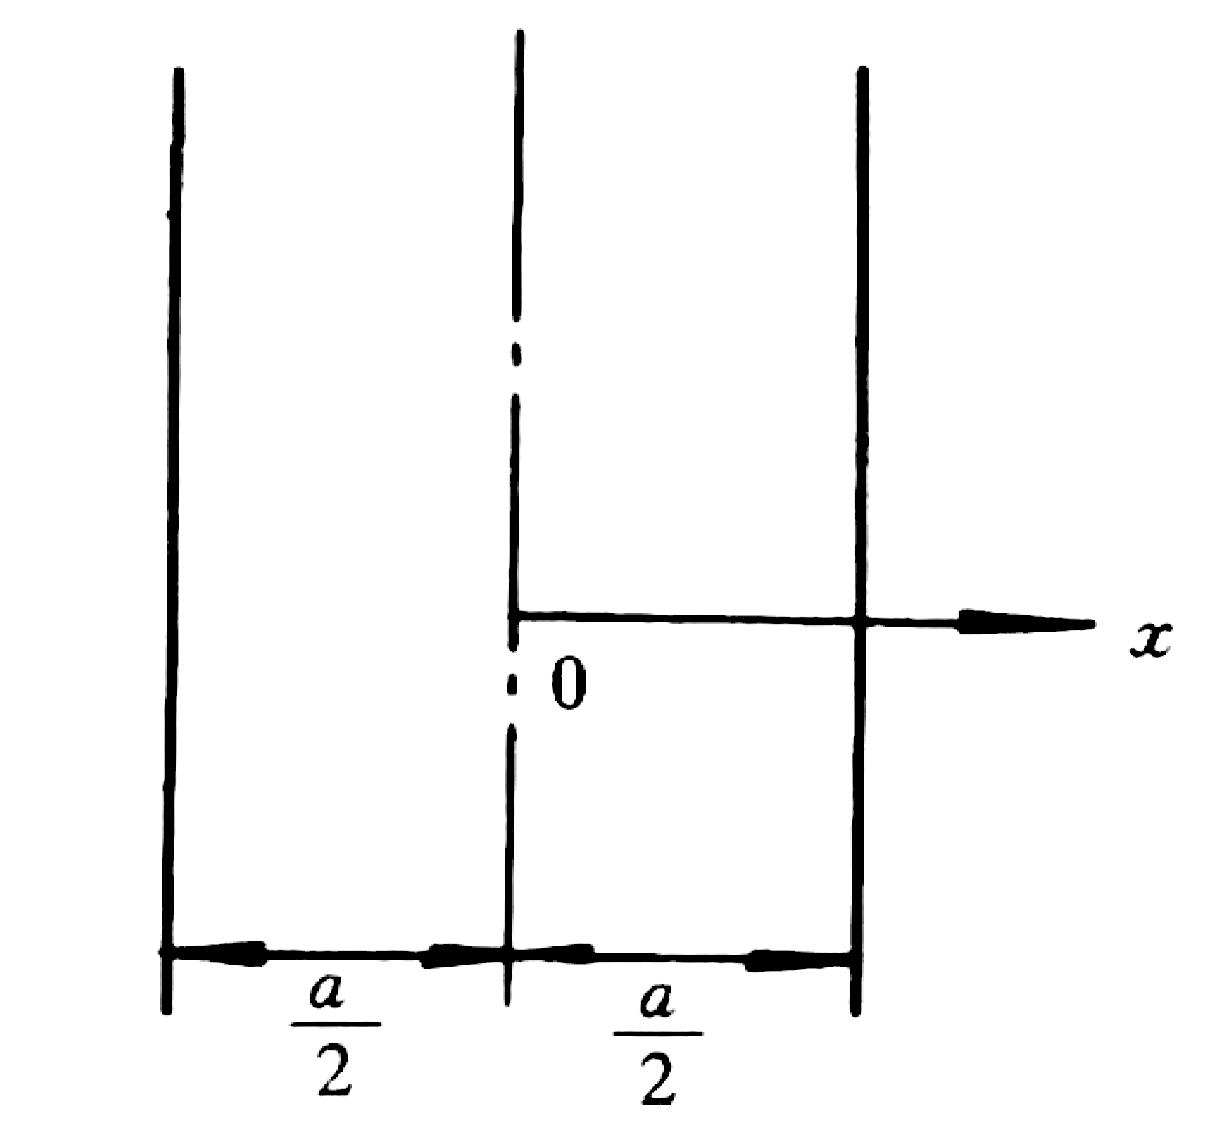
\includegraphics[width=0.3\textwidth]{./figure/无限平板形反应堆.png} % 替换为你的图片文件名
    \cnenfigcaption{无限平板形反应堆}{Infinite plate reactor}
    \vspace{3mm}
    \label{fig:无限平板形反应堆}
  \end{wrapfigure}

%%% 并排图
%%% 可在文中使用图\ref{fig1}、图\ref{fig2}引用图编号
% \begin{figure}[H]
%     \centering
%     \begin{minipage}[c]{0.48\textwidth}
%     \centering
%     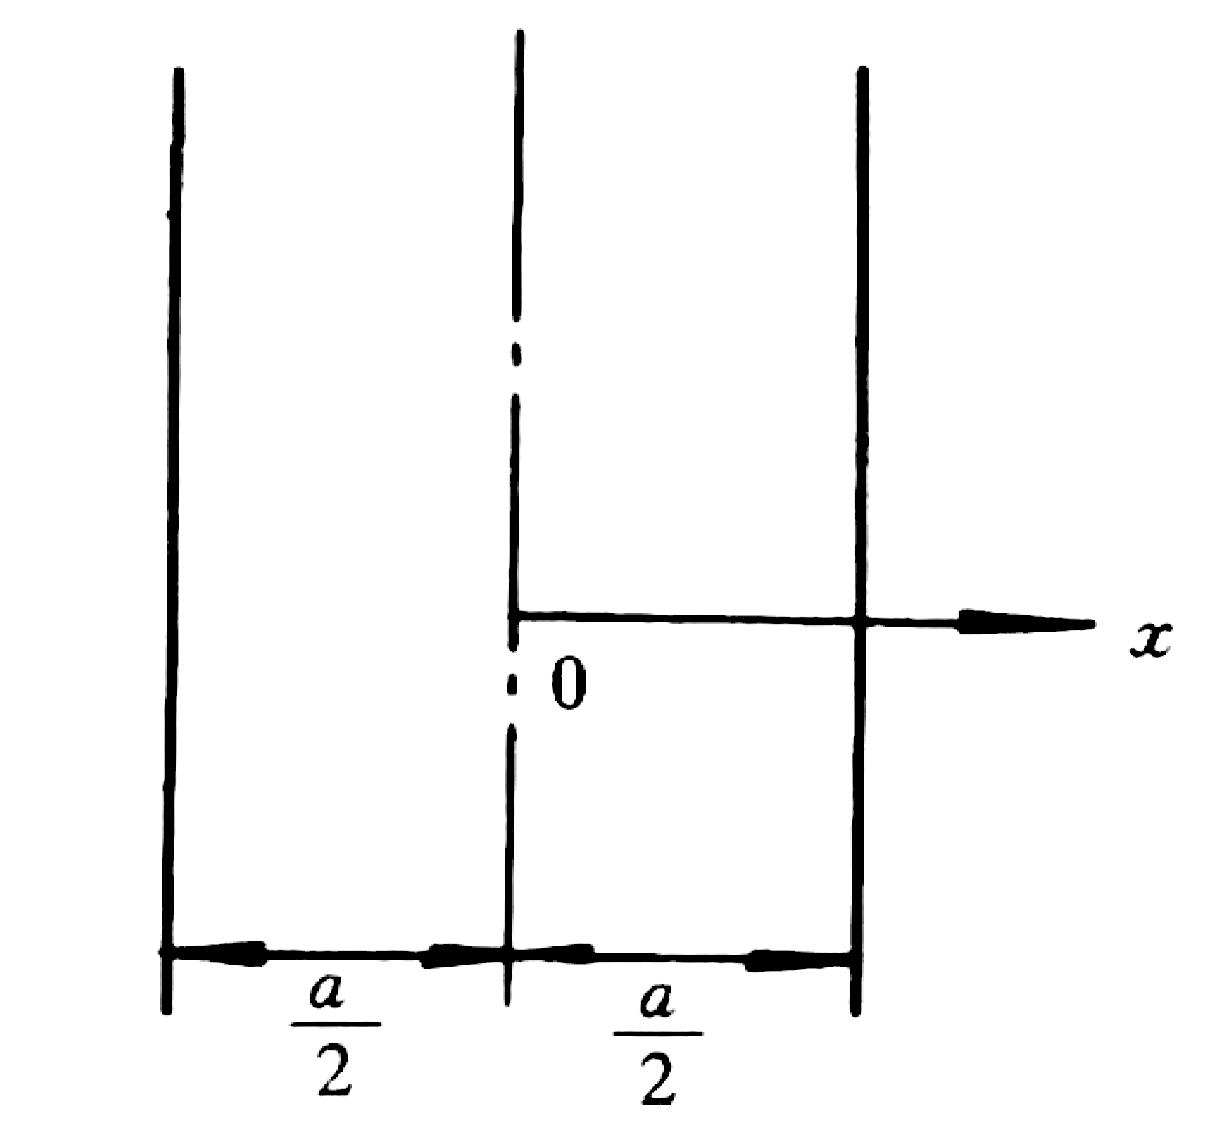
\includegraphics[width=0.8\textwidth]{./figure/无限平板形反应堆.png}
%     \end{minipage}
%     \hspace{0.02\textwidth}
%     \begin{minipage}[c]{0.48\textwidth}
%     \centering
%     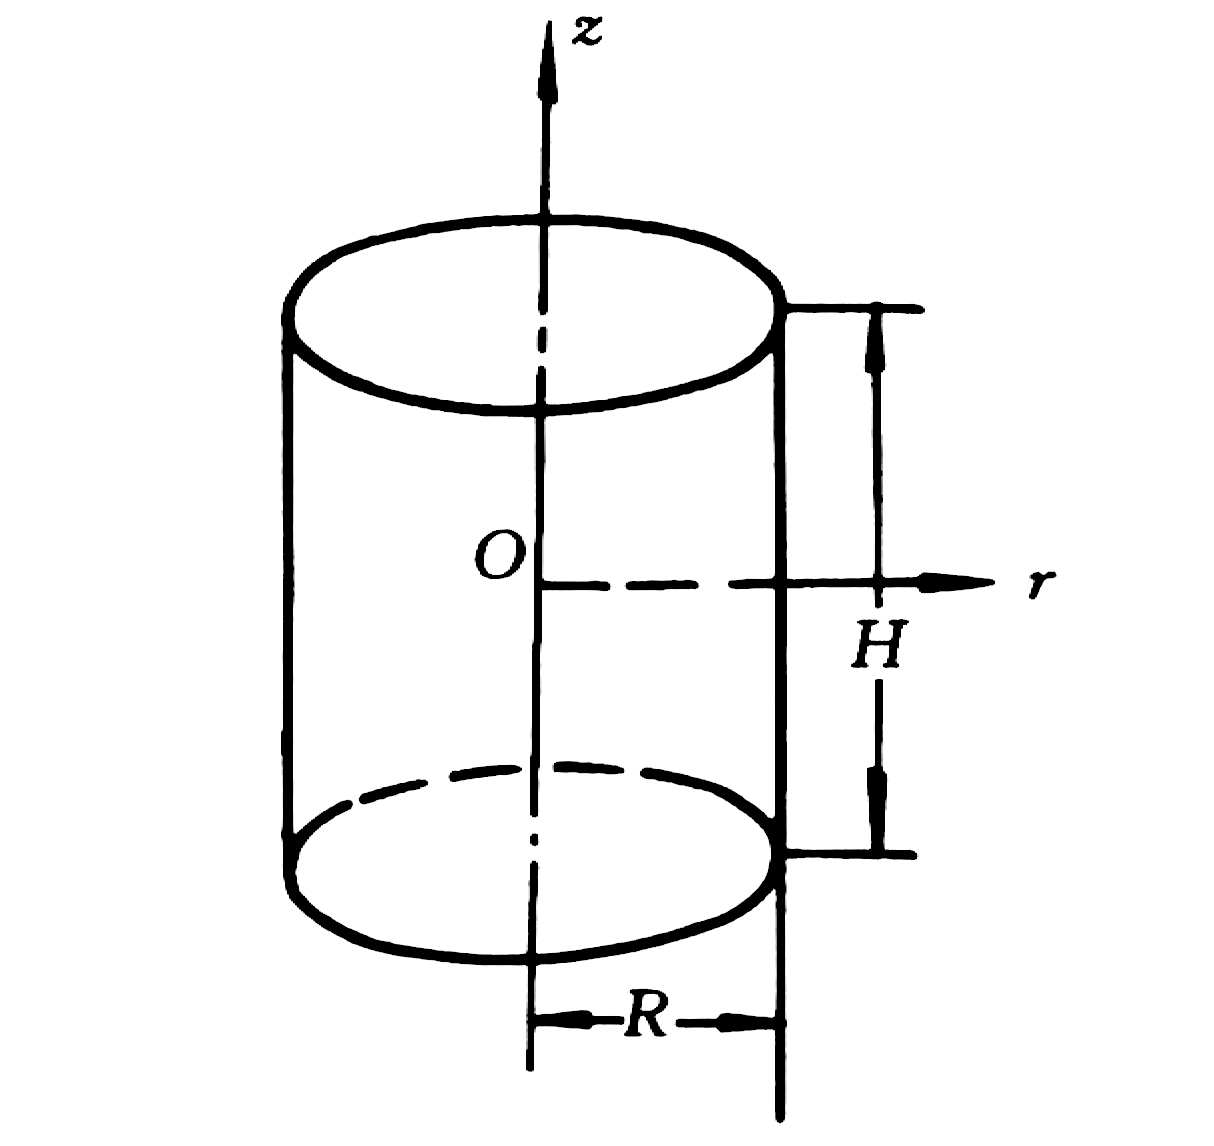
\includegraphics[width=0.8\textwidth]{./figure/圆柱体反应堆.png}
%     \end{minipage}\\[3mm]
%     \begin{minipage}[t]{0.48\textwidth}
%     \centering
%     \cnenfigcaption{无限平板形反应堆}{Infinite plate reactor}
%     \label{fig:无限平板形反应堆}
%     \end{minipage}
%     \hspace{0.02\textwidth}
%     \begin{minipage}[t]{0.48\textwidth}
%     \centering
%     \cnenfigcaption{圆柱体反应堆}{Cylindrical reactor}
%     \label{fig:圆柱体反应堆}
%     \end{minipage}
%     \end{figure}

在无外源的情况下,描述平板反应堆内中子通量密度变化规律的方程为
\begin{equation}
\frac{1}{v} \frac{\partial \phi(x, t)}{\partial t}=D \frac{\partial^2 \phi(x, t)}{\partial x^2}-\Sigma_{\mathrm{a}} \phi(x, t)+k_{\infty} \Sigma_{\mathrm{a}} \phi(x, t)
\label{eq:单群扩散方程43}
\end{equation}
其初始条件为
\begin{equation}
\phi(x, 0)=\phi_0(x)
\label{eq:初始条件44}
\end{equation}
边界条件为在反应堆外推边界处, 中子通量密度等于零, 即
\begin{equation}
\phi\left(\frac{a}{2}, t\right)=\phi\left(-\frac{a}{2}, t\right)=0
\label{eq:边界条件}
\end{equation}

注意这里已假设初始中子通量密度是对称的.用 $D$ 除式 \eqref{eq:单群扩散方程43}各项, 并注意到 $L^2=D / \Sigma_a$, 最后可得到
\begin{equation}
\frac{1}{D v} \frac{\partial \phi(x, t)}{\partial t}=\nabla^2 \phi(x, t)+\frac{k_{\infty}-1}{L^2} \phi(x, t)
\label{eq:单群扩散方程}
\end{equation}

这是一个二阶的偏微分方程, 对这类方程常可以采用分离变量法求解, 即求如下形式的解
\begin{equation}
\phi(x, t)=\varphi(x) T(t)
\label{eq:单群扩散方程的分离变量解}
\end{equation}
将式 \eqref{eq:单群扩散方程的分离变量解} 代入式 \eqref{eq:单群扩散方程} 中, 并用 $\varphi(x) T(t)$ 除方程中的各项,便得到
\begin{equation}
\frac{\nabla^2 \varphi(x)}{\varphi(x)}=\frac{1}{{Dv} T(t)} \frac{\mathrm{d} T(t)}{\mathrm{d} t}-\frac{k_{\infty}-1}{L^2}
\label{eq:单群扩散方程的分离变量解48}
\end{equation}
上式左端是仅含 $x$ 的函数, 而右端是仅含 $t$ 的函数, 因此要使等式成立, 等式两端必须都等于某一常数( 例如, $-B^2$ ).这样有
\begin{equation}
\frac{\nabla^2 \varphi(x)}{\varphi(x)}=-B^2
\end{equation}
或
\begin{equation}
\nabla^2 \varphi(x)+B^2 \varphi(x)=0
\label{eq:单群扩散方程的特征值问题}
\end{equation}

这里, $B^2$ 为一待定常数.式 \eqref{eq:单群扩散方程的特征值问题} 为典型的波动方程, $B^2$ 称为方程的 “特征值” .容易得出其通解为
\begin{equation}
\varphi(x)=A \cos B x+C \sin B x
\end{equation}
其中, $A$ 、 $C$ 为待定常数.由于初始通量密度分布 $\phi_0(x)$ 关于 $x=0$ 平面对称, 因此, 针对的问题只能选用满足对称性条件的解, 即
\begin{equation}
\varphi(x)=A \cos B x
\end{equation}

由边界条件式 \eqref{eq:边界条件}, 可导出 $\varphi(x)$ 应满足如下的边界条件: $\varphi\left( \pm \frac{a}{2}\right)=0$
\begin{equation}
A \cos \frac{B a}{2}=0
\end{equation}
因此要求
\begin{equation}
B_n=\frac{n \pi}{a} \quad n=1,3,5, \cdots
\end{equation}
或
\begin{equation}
B_n=\frac{(2 n-1) \pi}{a} \quad n=1,2,3, \cdots
\label{eq:单群扩散方程的特征值问题410}
\end{equation}

对应于其中的任一 $B_n$ 值, 都可以给出满足微分方程 \eqref{eq:单群扩散方程的特征值问题} 及边界条件 \eqref{eq:边界条件} 的解
\begin{equation}
\varphi_n(x)=A_n \cos B_n x=A_n \cos \frac{(2 n-1) \pi}{a} x
\label{eq:单群扩散方程的特征值问题解的无穷性}
\end{equation}

从上面的求解过程可以得出结论, 齐次方程 \eqref{eq:单群扩散方程的特征值问题} 只对某些特定的特征值 $B_n$ 才有解.相应的解 $\varphi_n(x)$ 称为此问题的特征函数.

下面接着来讨论方程 \eqref{eq:单群扩散方程的分离变量解48} 的求解, 由于特征函数的正交性 \footnote{单群特征函数的正交性可表示为 $\int_V \varphi_n(\boldsymbol{r}) \varphi_m(\boldsymbol{r}) \mathrm{d} V=0$, 当 $m \neq n$ 时.
}, 对于每一个 $n$ 值的项都是线性独立的, 因而对应每一个 $B_n^2$ 值和 $\varphi_n(x)$, 都有一个 $T_n(t)$ 与之对应, 由方程 \eqref{eq:单群扩散方程的分离变量解48} 得
\begin{equation}
\frac{1}{{Dv}T_n(t)} \frac{\mathrm{d} T_n(t)}{\mathrm{d} t}=\frac{k_{\infty}-1}{L^2}-B_n^2
\end{equation}

用 $L^2 /\left(1+L^2 B_n^2\right)$ 乘上式的每一项, 可以化简得到下列等式
\begin{equation}
\frac{1}{T_n(t)} \frac{\mathrm{d} T_n(t)}{\mathrm{d} t}=\frac{k_n-1}{l_n}
\label{eq:单群扩散方程的分离变量解412}
\end{equation}
其中
\begin{align}
l_n&=\frac{L^2}{Dv\left(1+L^2 B_n^2\right)}=\frac{l_{\infty}}{1+L^2 B_n^2} \label{eq:413}\\
k_n&=\frac{k_{\infty}}{1+L^2 B_n^2}\label{eq:414}
\end{align}
$l_{\infty}=\frac{\lambda_{\mathrm{a}}}{v}$ 为无限介质的热中子寿命, $\lambda_{\mathrm{a}}$ 是热中子的平均吸收自由程.方程 \eqref{eq:单群扩散方程的分离变量解412} 的解为
\begin{equation}
T_n=C_n \mathrm{e}^{\left(k_n-1\right) t / l_n}
\end{equation}
其中, $C_n$ 为待定常数.这样, 对于一维平板反应堆, 其中子通量密度的完全解就是对 $n=1$ 到 $n=\infty$ 的所有项的总和, 即
\begin{equation}
\phi(x, t)=\sum_{n=1}^{\infty} A_n^{\prime}\left[\cos \frac{(2 n-1) \pi}{a} x\right] \mathrm{e}^{\left(k_n-1\right) t / l_n}
\label{eq:单群扩散方程的分离变量解415}
\end{equation}
根据问题的初值条件式 \eqref{eq:初始条件44}, 可确定出上式中的待定系数 $A_n^{\prime}$ .为此, 令式中的 $t=0$, 可得
\begin{equation}
\phi_0(x)=\sum_{n=1}^{\infty} A_n^{\prime}\left[\cos \frac{(2 n-1) \pi}{a} x\right]
\end{equation}
利用正交关系,可求得
\begin{equation}
A_n^{\prime}=\frac{2}{a} \int_{-\frac{a}{2}}^{\frac{a}{2}} \phi_0(x) \cos \frac{(2 n-1) \pi}{a} x \mathrm{~d} x
\end{equation}
将其代入式 \eqref{eq:单群扩散方程的分离变量解415}, 可得到图 \ref{fig:无限平板形反应堆} 所示无限平板反应堆内的中子通量密度分布为
\begin{equation}
\phi(x, t)=\sum_{n=1}^{\infty}\left[\frac{2}{a} \int_{-\frac{a}{2}}^{\frac{a}{2}} \phi_0\left(x^{\prime}\right) \cos \frac{(2 n-1) \pi}{a} x^{\prime} \mathrm{d} x^{\prime}\right] \cos \frac{(2 n-1) \pi}{a} x \mathrm{e}^{\left(k_n-1\right) t / l_n}
\end{equation}
\subsubsection{热中子反应堆的临界条件}

通过前一小节的讨论可以知道, 特征值 $B_n^2$ 随 $n$ 的增加而单调增大, 最小特征值是 $n=1$ 时的 $B_1^2$ 值, 而同时又从式 \eqref{eq:414} 可以看出, 当 $n$ 增加时, $k_n$ 单调递减, 也就是说对应于最小特征值 $B_1^2$ 的 $k_1$ 是 $k_1, \cdots, k_n$ 中的最大值.另外, 从上一小节对平板反应堆的讨论可看出 $B_n^2$ 与系统尺寸有关, 当系统尺寸加大时, $B_n^2$ 便减小, 因而改变系统的尺寸就可以改变 $B_n^2$ 值, 从而也就改变了 $k_n$ 值.
分以下几种情况对式 \eqref{eq:单群扩散方程的分离变量解415}进行讨论.

第一种情况: 对于一定几何形状和体积的反应堆芯部, 若 $B_1^2$ 对应的 $k_1$ 小于 1 , 那么, 其余的 $k_2, \cdots, k_n$ 都将小于 1 , 这时所有的 $\left(k_n-1\right)$ 都是负值, 从式 \eqref{eq:单群扩散方程的分离变量解415} 可以看出, $\phi(x, t)$ 将随时间 $t$ 按指数规律衰减,因而系统处于次临界状态.

第二种情况: 若 $k_1>1$, 则 $\left(k_1-1\right)>0$, 这时中子通量密度将随时间不断地增长, 反应堆将处于超临界状态.

第三种情况: 若通过调整反应堆堆芯尺寸或改变反应堆内的材料成分, 使 $k_1$ 恰好等于 1 , 则其余 $k_2, \cdots, k_n(n>1)$ 的值都将小于 1 .这时式 \eqref{eq:单群扩散方程的分离变量解415} 中 $n=1$ 的项将与时间无关, 而 $n>1$ 的各项将随时间而衰减.因而当时间足够长时, $n>1$ 各项都已衰减到零, 系统达到稳态,
这时中子通量密度按基波形式 $\left(B=B_1\right)$ 分布, 反应堆处于临界状态.
从上面的讨论, 得到以下两个重要结果.

(1) 裸堆单群近似的“临界条件”为
\begin{equation}
k_1=\frac{k_{\infty}}{1+L^2 B^2}=1
\label{eq:单群扩散方程的特征值问题417}
\end{equation}
其中, $B^2$ 是波动方程 \eqref{eq:单群扩散方程的特征值问题} 的最小特征值 $B_1^2$, 通常把它记为 $B_{\mathrm{g}}^2$, 并称为几何曲率, 式 \eqref{eq:单群扩散方程的特征值问题417}称为单群理论的临界方程.显然, $k_1$ 便是前面定义的有效增殖系数.

(2) 当反应堆处于临界状态时, 中子通量密度按最小特征值 $B_{\mathrm{g}}^2$ 所对应的基波特征函数分布, 也就是说稳态反应堆的中子通量密度空间分布满足波动方程
\begin{equation}
\nabla^2 \phi(\boldsymbol{r})+B_{\mathrm{g}}^2 \boldsymbol{\phi}(\boldsymbol{r})=0
\label{eq:单群扩散方程的特征值问题418}
\end{equation}

这两点结论是非常重要的, 它们回答了反应堆临界时, 其材料组成、几何形状及大小之间必须怎样匹配? 还告诉一个临界反应堆内中子通量密度的分布.

下面仍以一维平板反应堆为例来加以具体讨论, 由式 \eqref{eq:单群扩散方程的特征值问题410} 及式 \eqref{eq:单群扩散方程的特征值问题417} 可得出无限平板反应堆的临界条件为
\begin{equation}
k_1=\frac{k_{\infty}}{1+L^2\left(\frac{\pi}{a}\right)^2}=1
\label{eq:单群扩散方程的特征值问题419}
\end{equation}

显然, 若系统的材料组成给定 (即 $k_{\infty}$ 、 $L^2$ 给定), 则只有一个唯一的尺寸 $a_0$ 能使 $k_1=1, a_0$ 即为反应堆的临界大小.当反应堆尺寸 $a>a_0$ 时, 则 $k_1>1$, 反应堆处于超临界状态; 反之, 若 $a<a_0$,则处于次临界状态.

另一方面, 若反应堆的尺寸 $a$ 给定, 则从式 \eqref{eq:单群扩散方程的特征值问题419} 可看出, 必然可以找到一种燃料富集度 (材料组成), 使得由其所确定的 $k_{\infty}$ 及 $L^2$ 值能使式 \eqref{eq:单群扩散方程的特征值问题419} 成立, 即 $k_1=1$, 从而反应堆达到临界状态.
临界时, 反应堆内的中子通量密度分布为
\begin{equation}
\phi(x)=A \cos \frac{\pi}{a} x
\label{eq:临界时反应堆内的中子通量密度分布}
\end{equation}

现在来讨论一下式 \eqref{eq:单群扩散方程的特征值问题417} 的物理意义.将证明式 \eqref{eq:单群扩散方程的特征值问题417} 中 $1 /\left(1+L^2 B_{\mathrm{g}}^2\right)$ 项的物理意义就是单群近似下反应堆内中子的不泄漏概率 $\Lambda$ .在反应堆中单位时间、单位体积内的中子泄漏率等于 $-D \boldsymbol{\nabla}^2 \phi$, 根据式 \eqref{eq:单群扩散方程的特征值问题418} 有 $-D \nabla^2 \phi=D B_g^2 \phi$, 而单位时间、单位体积内中子的吸收率为 $\Sigma_{\mathrm{a}} \phi$ .显然, 以单群理论观点来看, 反应堆内的中子不是从堆内泄漏出去, 就是在堆内被吸收,因而有
\begin{equation}
\begin{aligned}
\Lambda & =\frac{\text { 中子吸收率 }}{\text { 中子吸收率 }+ \text { 中子泄漏率 }} \\
& =\frac{\Sigma_{\mathrm{a}} \int_V \phi \mathrm{d} V}{\Sigma_{\mathrm{a}} \int_V \phi \mathrm{d} V+D B_{\mathrm{g}}^2 \int_V \phi \mathrm{d} V} \\
& =\frac{1}{1+L^2 B_{\mathrm{g}}^2}
\end{aligned}
\label{eq:单群扩散方程的特征值问题421}
\end{equation}
这样, 式 \eqref{eq:单群扩散方程的特征值问题417} 可以写成
\begin{equation}
k_1=k_{\infty} \Lambda=1
\end{equation}

它与临界条件式 \eqref{eq:反应堆维持自续链式裂变反应的条件} 完全一样.由此可见, 这里的 $k_1$ 也就是前面所定义的反应堆有效增殖系数 $k$ .同时, 由式 \eqref{eq:413} 可知, $l_1$ 为考虑热中子泄漏影响后的中子寿命.

另外, 从式 \eqref{eq:单群扩散方程的特征值问题421} 可以看出, 反应堆的中子泄漏不仅与扩散长度有关, 而且与几何曲率有关.从前面平板形反应堆的例子中可以看到, 当反应堆体积增大时, $B_g^2$ 就减小, 因而正如所预期的那样, 不泄漏概率也就增大.此外,扩散长度 $L$ 愈大, 意味着中子自产生到被吸收所穿行的距离也愈大, 因而从反应堆中泄漏出去的概率也就愈大, 不泄漏概率 $P_{\mathrm{L}}$ 就要减小, 这和式 \eqref{eq:单群扩散方程的特征值问题421} 的结果是一致的.
下面以一个简单例子说明上述结果的应用.

\begin{example}

     设有如图 \ref{fig:无限平板形反应堆} 所示的一维石墨慢化反应堆, $k_{\infty}=1.06, L^2=300 \mathrm{~cm}^2, \lambda_{\mathrm{tr}}=$ $2.8 \mathrm{~cm}$ .试求:

(1) 达到临界时反应堆的厚度 $H$ 和中子通量密度的分布;

(2) 设取 $H=250 \mathrm{~cm}$, 试求反应堆的有效增殖系数 $k_{\mathrm{eff}}$ .

解 (1) 根据式 \eqref{eq:单群扩散方程的特征值问题417} 的临界条件, 求得临界时反应堆的几何曲率 $B_{\mathrm{g}}^2$ 应为
\begin{equation}
B_g^2=\frac{k_{\infty}-1}{L^2}=\frac{1.06-1}{300}=2.0 \times 10^{-4} \mathrm{~cm}^{-2}
\end{equation}

因而 $B_{\mathrm{g}}=0.01414 \mathrm{~cm}^{-1}$, 另一方面根据式 \eqref{eq:单群扩散方程的特征值问题410} 有 $B_{\mathrm{g}}=\pi / a$, 因而有
\begin{equation}
a=\frac{\pi}{B_{\mathrm{g}}}=\frac{\pi}{0.01414}=222.2 \mathrm{~cm}
\end{equation}

由于外推距离 $d=0.7104 \lambda_{\mathrm{tr}}=0.7104 \times 2.8 \approx 2 \mathrm{~cm}$, 因而求得临界时反应堆的厚度
\begin{equation}
H=a-2 d=222.2-4=218.2 \mathrm{~cm}
\end{equation}

临界时中子通量密度分布为
\begin{equation}
\phi(x)=A \cos \frac{\pi}{a} x
\end{equation}

(2)若 $H=250 \mathrm{~cm}$, 则反应堆的几何曲率
\begin{equation}
B_{\mathrm{g}}^2=\left(\frac{\pi}{H+2 d}\right)^2=1.530 \times 10^{-4} \mathrm{~cm}^{-2}
\end{equation}

反应堆的有效增殖系数为
\begin{equation}
k_{\text {eff }}=\frac{k_{\infty}}{1+L^2 B_{\mathrm{g}}^2}=\frac{1.06}{1+300 \times 1.53 \times 10^{-4}}=1.0135
\end{equation}
    
\end{example}


从前面讨论知道, 平板形均匀裸堆内临界时的中子通量密度分布由方程 \eqref{eq:临界时反应堆内的中子通量密度分布} 确定, 其分布形状只取决于反应堆的几何形状, 而与反应堆的功率大小无关.这些式中都包含有待定的常数 $C$,也就是并未确定出反应堆内确切的中子通量密度大小.系数 $C$ 则需由反应堆的功率大小来确定.这是为什么呢? 这可以从波动方程 \eqref{eq:单群扩散方程的特征值问题418} 找到原因, 因为该方程是齐次方程, 所以, 若 $\phi(\boldsymbol{r})$ 是方程的一个解, 则 $\phi(\boldsymbol{r})$ 的任意倍数都是方程的解, 这样纯粹通过求解方程, 自然只能给出临界反应堆内中子通量密度的形状, 却不能给出通量密度的大小.实际上, 这蕴含着反应堆理论一个十分重要的结论, 那就是, 临界反应堆内中子通量密度的基波特征函数分布可以在任意功率水平下得到稳定.若不考虑各种工程因素的限制, 从物理原理上讲, 反应堆功率可以是任意大小,一个临界反应堆所能发出的功率并无任何限制.
    
反过来, 如已知反应堆的功率, 那么就可以确定出反应堆内中子通量密度的确切数值.设已知反应堆的功率为 $P$, 芯部的体积为 $V$, 每次裂变产生的能量为 $E_{\mathrm{f}}$, 则整个堆芯的总功率为
\begin{equation}
P=E_{\mathrm{f}} \int_V \Sigma_{\mathrm{f}} \phi(\boldsymbol{r}) \mathrm{d} V
\end{equation}

把有关反应堆内中子通量密度的表达式 \eqref{eq:临界时反应堆内的中子通量密度分布} 代入上式, 便可确定出常数 $C$ .
% \subsubsection{几种几何形状裸堆的几何曲率和中子通量密度分布} 

% 从前面讨论可以看到, 裸堆临界计算的关键在于求出各种几何形状和尺寸的反应堆系统的几何曲率 $B_{\mathrm{g}}^2$ 及其波动方程式 \eqref{eq:单群扩散方程的特征值问题418} 的基波解.下面推导几种最常见的几何形状反应堆的几何曲率及临界时的中子通量密度分布函数.

% 1. 球形反应堆

% 考虑一个半径为 $R$ (包括外推距离在内) 的球形裸堆, 应用球坐标系统, 并把原点取在球心上.由于通量密度关于极角 $\theta$ 和辐角 $\varphi$ 都是对称的, 因此波动方程式 \eqref{eq:单群扩散方程的特征值问题418} 为
% \begin{equation}
% \frac{\mathrm{d}^2 \phi(r)}{\mathrm{d} r^2}+\frac{2}{r} \frac{\mathrm{d} \phi(r)}{\mathrm{d} r}+B_{\mathrm{g}}^2 \phi(r)=0
% \end{equation}
% 上式的普遍解 (见表 \ref{tab:几种几何形状的裸堆的几何曲率和热中子通量密度分布}) 为
% \begin{equation}
% \phi(r)=C \frac{\sin B_{\mathrm{g}} r}{r}+E \frac{\cos B_{\mathrm{g}} r}{r}
% \label{eq:单群扩散方程的特征值问题422}
% \end{equation}

% 为了满足当 $r$ 趋近于零时, 中子通量密度为有限值的条件, 常数 $E$ 必须为零.所以式 \eqref{eq:单群扩散方程的特征值问题422}的解为
% \begin{equation}
% \phi(r)=C \frac{\sin B_g r}{r}
% \end{equation}

% 根据 $\phi(R)=0$ 的边界条件的要求, 必须使 $B_{\mathrm{g}} R=n \pi, n=1,2,3, \cdots$ .因此对应于 $n=1$ 的最小特征值, 几何曲率 $B_{\mathrm{g}}^2$ 为
% \begin{equation}
% B_{\mathrm{g}}^2=\left(\frac{\pi}{R}\right)^2
% \end{equation}
% 与此相应的临界反应堆内的中子通量密度分布为
% \begin{equation}
% \phi(r)=C \frac{\sin \left(\frac{\pi r}{R}\right)}{r}
% \label{相应的临界反应堆内的中子通量密度分布425}
% \end{equation}其中, $C$ 为常数, 它由中子通量密度的归一化条件或反应堆的输出功率决定.

% 2. 有限高圆柱体反应堆

% 圆柱体为最常见的反应堆形状.设圆柱体反应堆的半径为 $R$, 高度为 $H(R, H$ 均包括外推距离在内), 如图 \ref{fig:圆柱体反应堆} 所示.采用柱坐标系, 原点取在圆柱体轴线的中点上, 这时中子通量密度只取决于 $r$ 和 $z$ 两个变量, 波动方程便写成

% \begin{equation}
% \frac{\partial^2 \phi(r, z)}{\partial r^2}+\frac{1}{r} \frac{\partial \phi(r, z)}{\partial r}+\frac{\partial^2 \phi(r, z)}{\partial z^2}+B_{\mathrm{g}}^2 \phi(r, z)=0
% \label{eq:单群扩散方程的特征值问题426}
% \end{equation}
%    %%% 图文并排
%    \begin{wrapfigure}{r}{0.3\textwidth}
%     \centering
%     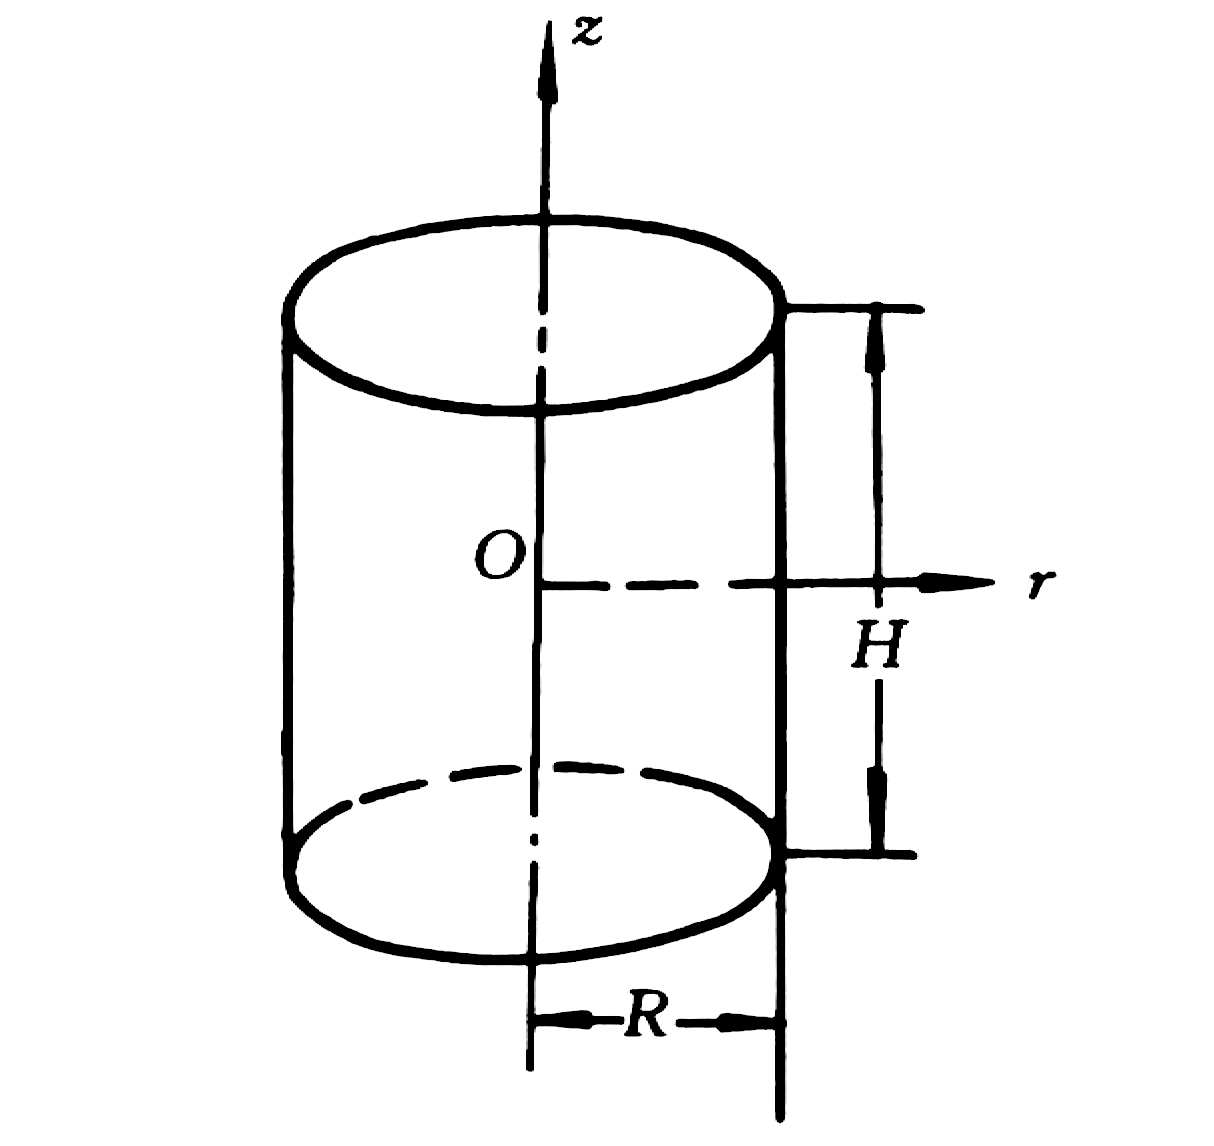
\includegraphics[width=0.3\textwidth]{./figure/圆柱体反应堆.png} % 替换为你的图片文件名
%     \cnenfigcaption{圆柱体反应堆}{Cylindrical reactor}
%     \vspace{3mm}
%     \label{fig:圆柱体反应堆}
%   \end{wrapfigure} 
% 该问题的定解条件是

% (1) 中子通量密度在堆内各处均为有限值;

% (2) 当 $r=R$ 或 $z= \pm \frac{H}{2}$ 时, $\phi(r, z)=0$ .

% 采用分离变量法求解, 把 $\phi(r, z)$ 分离变量写成
% \begin{equation}
% \phi(r, z)=\varphi(r) Z(z)
% \end{equation}
% 把它代入式 \eqref{eq:单群扩散方程的特征值问题426}, 并用 $\varphi(r) Z(z)$ 除式中各项得到
% \begin{equation}
% \frac{1}{\varphi(r)}\left[\frac{\mathrm{d}^2 \varphi(r)}{\mathrm{d} r^2}+\frac{1}{r} \frac{\mathrm{d} \varphi(r)}{\mathrm{d} r}\right]+\frac{1}{Z(z)} \frac{\mathrm{d}^2 Z(z)}{\mathrm{d} z^2}=-B_{\mathrm{g}}^2
% \end{equation}
% 因而可以令左端每一项均等于常数,有
% \begin{align}
% \frac{1}{\varphi(r)}\left[\frac{\mathrm{d}^2 \varphi(r)}{\mathrm{d} r^2}+\frac{1}{r} \frac{\mathrm{d} \varphi(r)}{\mathrm{d} r}\right]=-B_r^2 \label{eq:单群扩散方程的特征值问题427}\\
% \frac{1}{Z(z)} \frac{\mathrm{d}^2 Z(z)}{\mathrm{d} z^2}=-B_z^2\label{eq:单群扩散方程的特征值问题428}
% \end{align}
% 以及
% \begin{equation}
% B_{\mathrm{k}}^2=B_{\mathrm{r}}^2+B_{\mathrm{z}}^2
% \end{equation}
% 现在求解式 \eqref{eq:单群扩散方程的特征值问题427} .令 $x=B_r r$, 将其代入式 \eqref{eq:单群扩散方程的特征值问题427} 中去, 便得到所熟悉的零阶贝塞尔方程
% \begin{equation}
% x^2 \frac{\mathrm{d}^2 \varphi(x)}{\mathrm{d} x^2}+x \frac{\mathrm{d} \varphi(x)}{\mathrm{d} x}+x^2 \varphi(x)=0
% \end{equation}
% 其普遍解为
% \begin{equation}
% \varphi(r)=A \mathrm{~J}_0\left(B_{\mathrm{r}} r\right)+E \mathrm{Y}_0\left(B_{\mathrm{r}} r\right)
% \end{equation}其中, $\mathrm{J}_0 、 \mathrm{Y}_0$ 分别为第一类及第二类零阶贝塞尔函数.
% 如果假设式 \eqref{eq:单群扩散方程的特征值问题427} 右端等于正数, 则它将化成一个零阶修正贝塞尔方程
% \begin{equation}
% x^2 \frac{\mathrm{d}^2 \varphi(x)}{\mathrm{d} x^2}+x \frac{\mathrm{d} \varphi(x)}{\mathrm{d} x}-x^2 \varphi(x)=0
% \end{equation}
% 它的普遍解是
% \begin{equation}
% \varphi(r)=A^{\prime} \mathrm{I}_0\left(B_{\mathrm{r}} r\right)+E^{\prime} \mathrm{K}_0\left(B_{\mathrm{r}} r\right)
% \end{equation}其中, $\mathrm{I}_0 、 \mathrm{~K}_0$ 分别为第一类和第二类零阶修正贝塞尔函数.图 \ref{fig:零阶贝赛尔函数曲线} 中画出了 $\mathrm{J}_0 、 \mathrm{Y}_0 、 \mathrm{I}_0$ 和 $\mathrm{K}_0$ 的曲线.根据该问题的定解条件 (1) 和 (2), 从这些曲线上可以看出, $\mathrm{Y}_0 、 \mathrm{I}_0$ 和 $\mathrm{K}_0$ 均应从上述解中消去, 因而在式 \eqref{eq:单群扩散方程的特征值问题427} 右端项常数必须取 $-B_r^2$ 值.故式 \eqref{eq:单群扩散方程的特征值问题427} 的允许解为

% \begin{figure}[H]
%     \centering
%     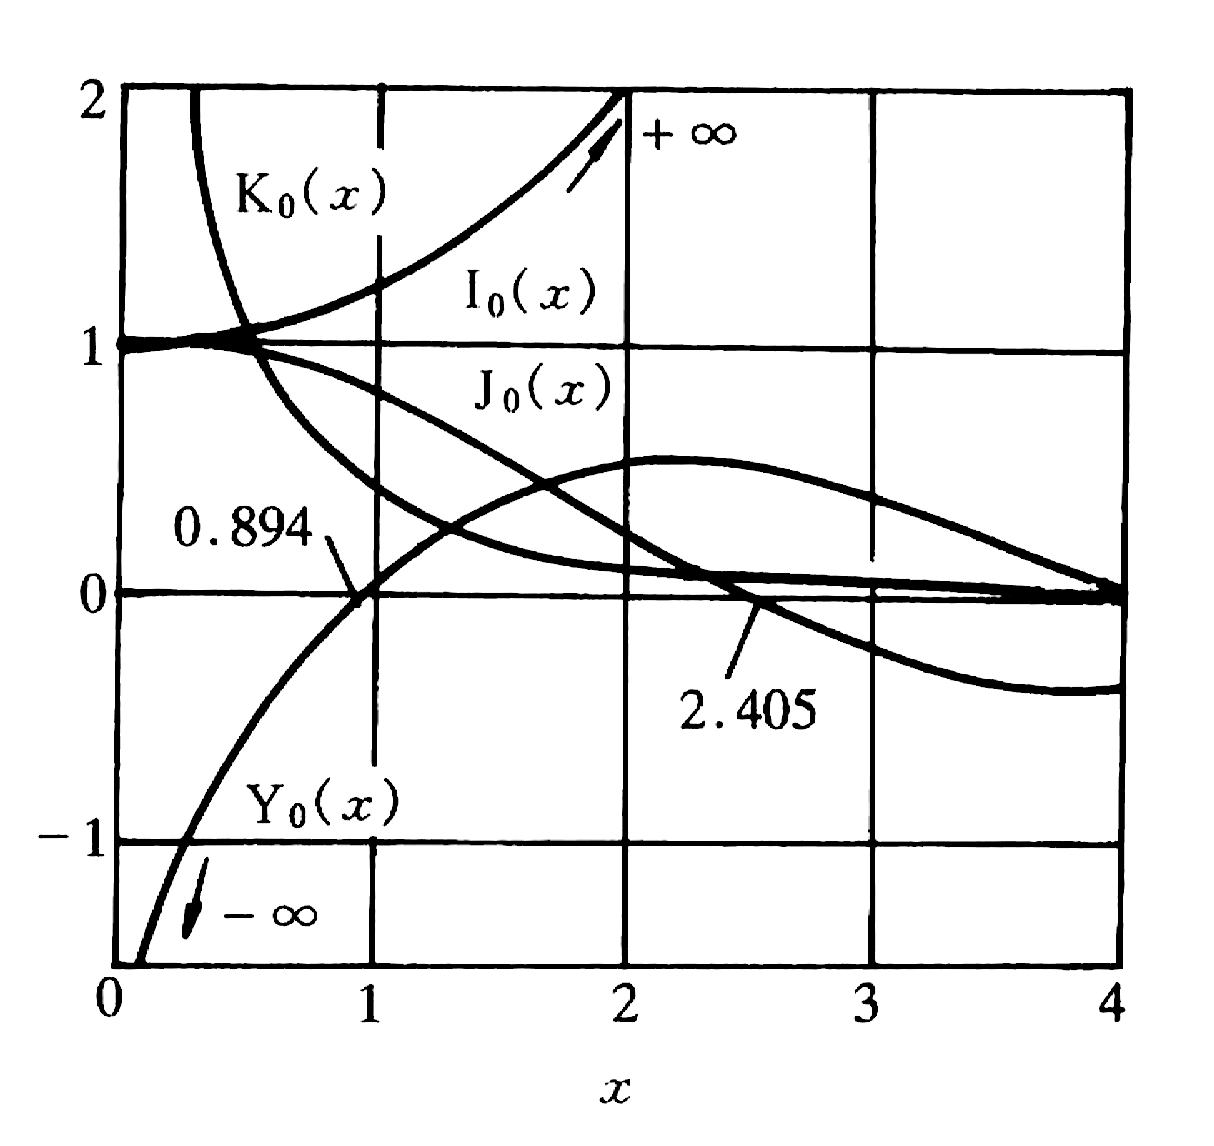
\includegraphics[width=0.6\textwidth]{./figure/零阶贝赛尔函数曲线.png}
%     \cnenfigcaption{零阶贝赛尔函数曲线}{Zero order Bessel function curve}
%     \label{fig:零阶贝赛尔函数曲线}
%     \end{figure}

% \begin{equation}
% \varphi(r)=A \mathrm{~J}_0\left(B_{\mathrm{r}} r\right)
% \end{equation}

% 为了计算 $B_{\mathrm{r}}^2$, 可以利用在 $r=R$ 处, $\phi(r, z)=0$ 的边界条件, 即
% \begin{equation}
% \varphi(R)=A \mathrm{~J}_0\left(B_{\mathrm{r}} R\right)=0
% \end{equation}其中, 常数 $A$ 不能为零, 故只能是 $\mathrm{J}_0\left(B_{\mathrm{r}} R\right)=0$, 由图 \ref{fig:零阶贝赛尔函数曲线} 知贝塞尔函数 $\mathrm{J}_0$ 的第一个零点是 2.405 , 因而
% \begin{equation}
%     B_{\mathrm{r}}^2=\left(\frac{2.405}{R}\right)^2
% \end{equation}
% 因此有
% \begin{equation}
%     \varphi(r)=A \mathrm{~J}_0\left(B_{\mathrm{r}} r\right)=A \mathrm{~J}_0\left(\frac{2.405}{R} r\right)
% \end{equation}
% 接着求解方程 \eqref{eq:单群扩散方程的特征值问题428}, 由前面平板形反应堆的讨论已经知道它的解为
% \begin{equation}
% Z(z)=F \cos B_z z
% \end{equation}其中
% \begin{equation}
% B_z^2=\left(\frac{\pi}{H}\right)^2
% \end{equation}
% 这样, 圆柱体裸堆的几何曲率为
% \begin{equation}
% B_{\mathrm{g}}^2=B_{\mathrm{r}}^2+B_z^2=\left(\frac{2.405}{R}\right)^2+\left(\frac{\pi}{H}\right)^2
% \end{equation}其中, $B_r^2$ 称为径向几何曲率; $B_z^2$ 称为轴向几何曲率.
% 因而有限高圆柱体裸堆的中子通量密度的分布形式为
% \begin{equation}
% \begin{aligned}
% \phi(r, z) & =C \mathrm{~J}_0\left(B_{\mathrm{r}} r\right) \cos \left(B_z z\right) \\
% & =C \mathrm{~J}_0\left(\frac{2.405}{R} r\right) \cos \left(\frac{\pi}{H} z\right)
% \end{aligned}
% \label{eq:单群扩散方程的特征值问题436}
% \end{equation}其中, 常数 $C$ 是由中子通量密度的归一条件或反应堆的输出功率来确定的.

% 利用求条件极值的方法可以求出, 在给定的 $B_{\mathrm{g}}^2$ 值下, 当直径 $D=1.083 \mathrm{H}$ 时, 圆柱体反应堆具有最小临界体积.

% 同样方法可以求出边长为 $(a, b, c)$ 的长方体裸堆的几何曲率和中子通量密度分布.下面将上述几种几何形状反应堆的几何曲率与中子通量密度分布总结列于表 \ref{tab:几种几何形状的裸堆的几何曲率和热中子通量密度分布} 中.
% \begin{table}[H]
%     \caption{几种几何形状的裸堆的几何曲率和热中子通量密度分布}
%     \label{tab:几种几何形状的裸堆的几何曲率和热中子通量密度分布}
%     \centering
%     \begin{tabular}{c|c|c}
%     \toprule
%     几何形状 & 几何曲率 & 热中子通量密度分布 \\
%     \hline
%     球形 (半径 $R$) & $B_{\mathrm{g}}^2=\left(\frac{\pi}{R}\right)^2$ & $\frac{1}{r} \sin \left(\frac{\pi}{R} r\right)$ \\
%     \hline
%     \begin{tabular}{@{}c@{}}
%     直角长方体 \\
%     (边长: $a, b, c$)
%     \end{tabular} & 
%     \begin{tabular}{@{}c@{}}
%     $B_g^2=B_x^2+B_y^2+B_z^2$ \\
%     $B_g^2=\left(\frac{\pi}{a}\right)^2+\left(\frac{\pi}{b}\right)^2+\left(\frac{\pi}{c}\right)^2$
%     \end{tabular} & $\cos \left(\frac{\pi}{a} x\right) \cos \left(\frac{\pi}{b} y\right) \cos \left(\frac{\pi}{c} z\right)$ \\
%     \hline
%     \begin{tabular}{@{}c@{}}
%     圆柱体 \\
%     (半径 $R$, 高 $H$)
%     \end{tabular} & 
%     \begin{tabular}{@{}c@{}}
%     $B_{\mathrm{g}}^2=B_{\mathrm{r}}^2+B_{\mathrm{z}}^2$ \\
%     $B_{\mathrm{g}}^2=\left(\frac{2.405}{R}\right)^2+\left(\frac{\pi}{H}\right)^2$
%     \end{tabular} & $\mathrm{J}_0\left(\frac{2.405}{R} r\right) \cos \left(\frac{\pi}{H} z\right)$ \\
%     \bottomrule
%     \end{tabular}
%     \end{table}
    
    
%     从前面讨论知道, 均匀裸堆内临界时的中子通量密度分布由方程 \eqref{相应的临界反应堆内的中子通量密度分布425} 、式 \eqref{eq:单群扩散方程的特征值问题436}等确定, 其分布形状只取决于反应堆的几何形状, 而与反应堆的功率大小无关.例如, 对于所有圆柱体堆, 其径向中子通量密度分布均服从贝塞尔函数分布.这些式中都包含有待定的常数 $C$,也就是并未确定出反应堆内确切的中子通量密度大小.系数 $C$ 则需由反应堆的功率大小来确定.这是为什么呢? 这可以从波动方程 \eqref{eq:单群扩散方程的特征值问题418} 找到原因, 因为该方程是齐次方程, 所以, 若 $\phi(\boldsymbol{r})$ 是方程的一个解, 则 $\phi(\boldsymbol{r})$ 的任意倍数都是方程的解, 这样纯粹通过求解方程, 自然只能给出临界反应堆内中子通量密度的形状, 却不能给出通量密度的大小.实际上, 这蕴含着反应堆理论一个十分重要的结论, 那就是, 临界反应堆内中子通量密度的基波特征函数分布可以在任意功率水平下得到稳定.若不考虑各种工程因素的限制, 从物理原理上讲, 反应堆功率可以是任意大小,一个临界反应堆所能发出的功率并无任何限制.
    
%     反过来, 如已知反应堆的功率, 那么就可以确定出反应堆内中子通量密度的确切数值.设已知反应堆的功率为 $P$, 芯部的体积为 $V$, 每次裂变产生的能量为 $E_{\mathrm{f}}$, 则整个堆芯的总功率为
%     \begin{equation}
%     P=E_{\mathrm{f}} \int_V \Sigma_{\mathrm{f}} \phi(\boldsymbol{r}) \mathrm{d} V
% \end{equation}
    
%     把有关反应堆内中子通量密度的表达式 \eqref{相应的临界反应堆内的中子通量密度分布425} 或式 \eqref{eq:单群扩散方程的特征值问题436} 代入上式, 便可确定出常数 $C$ .对于圆柱体裸堆, $V=\pi R^2 H$, 有
%     \begin{equation}
%     \begin{gathered}
%     P=E_{\mathrm{i}} \Sigma_{\mathrm{i}} C \int_0^R \int_0^{\frac{H}{2}} 2 \mathrm{~J}_0\left(\frac{2.405 r}{R}\right) \cos \left(\frac{\pi Z}{H}\right) 2 \pi r \mathrm{~d} r \mathrm{~d} z=\frac{2.07 V E_{\mathrm{i}} \Sigma_{\mathrm{i}} C}{2.405 \pi} \\
%     C=\frac{3.64 P}{V E_{\mathrm{i}} \Sigma_{\mathrm{i}}}
%     \end{gathered}
% \end{equation}
%     同样对于球形裸堆, $V=4 \pi R^3 / 3$, 有
%     \begin{equation}
%     C=\frac{3.29 P}{V E_{\mathrm{i}} \Sigma_{\mathrm{f}}}
% \end{equation}

% \begin{remark}\quad

% \begin{itemize}
%     \item 贝塞尔函数
% 贝塞尔方程为
% \begin{equation}
% x^2 f^{\prime \prime}+x f^{\prime}+\left(x^2-n^2\right) f=0
% \end{equation}

% 若 $n$ 为整数或零, 它的两个解为
% \begin{equation}
% \begin{gathered}
% f(x)=\left\{\begin{array}{l}
% \mathrm{J}_n(x) \\
% \mathrm{Y}_n(x)
% \end{array}\right. \\
% \mathrm{J}_n(x)=\sum_{k=0}^{\infty} \frac{(-1)^k}{\Gamma(k+1) \Gamma(k+n+1)}\left(\frac{x}{2}\right)^{n+2 k} \\
% \mathrm{Y}_n(x)=\frac{\mathrm{J}_n(x) \cos (n \pi)-\mathrm{J}_n(x)}{\sin (n \pi)}
% \end{gathered}
% \end{equation}

% 函数 $\mathrm{J}_n(x)$ 和 $\mathrm{Y}_n(x)$ 分别称为第一类和第二类贝塞尔函数. $\mathrm{J}_0(x)$ 和 $\mathrm{Y}_0(x)$ 如图 \ref{fig:零阶贝赛尔函数曲线} 所示.
% \item 修正贝塞尔函数
% 修正贝塞尔方程为
% \begin{equation}
% x^2 f^{\prime \prime}+x f^{\prime}-\left(x^2+n^2\right) f=0
% \end{equation}

% 若 $n$ 为整数或零, 它的两个解为
% \begin{equation}
% f(x)=\left\{\begin{array}{l}
% \mathrm{I}_n(x) \\
% \mathrm{K}_n(x)
% \end{array}\right.
% \end{equation}

% 其中
% \begin{equation}
% \begin{gathered}
% \mathrm{I}_n(x)=i^{-n} \mathrm{~J}_n(i x)=i^n \mathrm{~J}_n(-i x) \\
% \mathrm{K}_n(x)=\frac{\pi}{2} i^{n+1}\left[\mathrm{~J}_n(i x)+i \mathrm{Y}_n(i x)\right]
% \end{gathered}
% \end{equation}

% 函数 $\mathrm{I}_n(x)$ 和 $\mathrm{K}_n(x)$ 分别称为第一类和第二类修正贝塞尔函数. $\mathrm{I}_0(x)$ 和 $\mathrm{K}_0(x)$ 如图 \ref{fig:零阶贝赛尔函数曲线} 所示.
% \end{itemize}
% \end{remark}

\subsubsection{反应堆曲率和临界计算任务}
    
    从前面的讨论知道, 稳态反应堆内中子通量密度的空间分布满足波动方程, 即
    \begin{equation}
\nabla^2 \phi(\boldsymbol{r})+B_{\mathrm{g}}^2 \phi(\boldsymbol{r})=0
\end{equation}

这里, $B_{\mathrm{g}}^2$ 为方程的最小特征值, 即几何曲率.对于裸堆来讲, 几何曲率只与反应堆的几何形状和尺寸大小有关, 例如对于平板形裸堆, $B_{\mathrm{g}}^2=\left(\frac{\pi}{a}\right)^2$, 它与反应堆的材料成分和性质没有关系.对于处在临界状态的反应堆, 它的几何曲率应能满足临界方程 \eqref{eq:单群扩散方程的特征值问题417}.

另一方面, 由于 $k_{\infty}$ 、 $L^2$ 等参数都仅仅取决于反应堆芯部材料特性, 因而, 对于一定材料成分 (即给定 $k_{\infty}$ 、 $L^2$ 等值) 的反应堆, 便有一个确定的 $B^2$ 值能满足临界方程 \eqref{eq:单群扩散方程的特征值问题417}.为了计算和讨论方便, 把它叫作材料曲率, 它是满足临界方程 \eqref{eq:单群扩散方程的特征值问题417} 的 $B^2$ 值, 并记作 $B_{\mathrm{m}}^2$ .因而,对于单群扩散理论, 材料曲率 $B_{\mathrm{m}}^2$ 为
\begin{equation}
B_{\mathrm{m}}^2=\frac{k_{\infty}-1}{L^2}
\end{equation}
显然, 材料曲率 $B_{\mathrm{m}}^2$ 反映增殖介质材料的特性, 它的数值只取决于反应堆的材料成分和特性 (如 $L^2$ 、 $\tau$ 、 $k_{\infty}$ 等), 而与反应堆的几何形状及大小无关.显然, 对于任意给定材料成分和几何尺寸的反应堆, 几何曲率不一定等于材料曲率.

因而引进了材料曲率的概念之后, 反应堆的临界条件可以描写如下: 反应堆达到临界的条件是材料曲率等于几何曲率, 即
\begin{equation}
B_{\mathrm{m}}^2=B_{\mathrm{g}}^2
\label{eq:单群扩散方程的特征值问题443}
\end{equation}

% 例如, 对于裸堆情况, 利用单群理论, 可以将临界条件式 \eqref{eq:445}的具体形式写成

% \begin{align}
% & \frac{k_{\infty}-1}{L^2}=\left(\frac{\pi}{R}\right)^2 \quad(\text { 对球形裸堆) } \label{eq:444}\\
% & \frac{k_{\infty}-1}{L^2}=\left(\frac{\pi}{H}\right)^2+\left(\frac{2.405}{R}\right)^2 \quad \text { (对圆柱体裸堆) }\label{eq:445}
% \end{align}

在一般情况下, 对于给定尺寸的反应堆, 其几何曲率 $B_{\mathrm{g}}^2$ 不一定等于材料曲率 $B_{\mathrm{m}}^2$ .若 $B_{\mathrm{g}}^2<B_{\mathrm{m}}^2$, 这时 $k$ 将大于 1 , 反应堆处于超临界状态; 反之, 若 $B_{\mathrm{g}}^2>B_{\mathrm{m}}^2$, 则反应堆处于次临界状态.
最后, 由上面的讨论可清楚地看到, 反应堆临界问题的计算可以归纳为下面两类问题.

第一类问题: 给定反应堆材料成分, 确定它的临界尺寸.当反应堆的材料成分给定以后, $k_{\infty}$ 、 $L^2$ 等物理参数便可以很容易地计算出来.因而, 材料曲率就成为已知的量, 问题便成了求临界尺寸问题.临界时, $B_{\mathrm{m}}^2=B_{\mathrm{g}}^2$, 可以根据 $B_{\mathrm{g}}^2$ 与尺寸的关系式计算出临界尺寸来.

第二类问题: 给定了反应堆的形状和尺寸, 确定临界时反应堆的材料成分.这时, 事先给定反应堆的几何形状和尺寸 (例如, 由热工计算给出), 而要求临界时所需的材料成分 (一般是燃料的富集度).事实上这是第一种情况的逆问题, 因为这时几何曲率 $B_{\mathrm{g}}^2$ 是已知的, 所需要的是改变反应堆的燃料一慢化剂成分和比例, 以使得临界方程 \eqref{eq:单群扩散方程的特征值问题417}得到满足.

在具体计算中, 有时还会遇到这样的情况, 即不仅反应堆的材料成分 (如燃料一慢化剂) 已经给定, 而且反应堆的几何尺寸亦已由工程或热工的需要所确定.这时需要求的是反应堆的有效增殖系数
\begin{equation}
k_{\mathrm{eff}}=\frac{k_{\infty}}{1+L^2 B_{\mathrm{g}}^2}
\end{equation}
或
\begin{equation}
\rho=\frac{k-1}{k}
\end{equation}
其中, $\rho$ 通常称为反应性.对于临界反应堆, $\rho=0$; 若 $\rho>0$, 则反应堆处于超临界状态; 若 $\rho<0$,则反应堆处于次临界状态.因此 $|\rho|$ 的大小表示反应堆偏离临界状态的程度.
\subsubsection{单群理论的修正}
前面提到, 单群理论是一种近似的方法.计算表明, 对于热中子反应堆, 直接应用式 \eqref{eq:单群扩散方程的特征值问题417} 或式 \eqref{eq:单群扩散方程的特征值问题443} 进行计算, 将带来比较大的误差.
但是, 计算若用 $M^2=L^2+\tau$ 来替换上述式中的 $L^2$, 则可以改善计算结果, 使其更令人满意.这样, 临界条件和材料曲率便改写成下列形式:
\begin{equation}
\begin{gathered}
k_{\mathrm{eff}}=\frac{k_{\infty}}{1+M^2 B_{\mathrm{g}}^2}=1 \\
B_{\mathrm{m}}^2=\frac{k_{\infty}-1}{M^2}
\end{gathered}
\end{equation}

这就是所谓的热中子反应堆的修正单群理论.
修正单群理论之所以能改善计算结果, 其主要原因可以从物理上解释如下: 在单群理论中, 把所有中子都看成是热中子, 因而该理论没有考虑慢化过程对中子泄漏的影响.知道, $L^2$ 与中子从变成热中子地点开始到它被吸收为止所移动过的距离有关, $1 /\left(1+L^2 B_{\mathrm{g}}^2\right)$ 为热中子扩散过程中的不泄漏概率.但是, 在反应堆内, 实际上中子由裂变中子慢化成为热中子之前, 已经移动过了一个距离 $\tau$, 而徙动面积 $M^2=L^2+\tau$ 跟中子由核裂变产生直到它被吸收所穿行距离的均方值有关, 故若用徙动面积 $M^2=L^2+\tau$ 来代替 $L^2$, 便可初步地考虑慢化过程对泄漏的影响, 因而使计算精度得到改善.实际计算结果也证明了这一结论.因此, 以后提到单群理论一般都是指应用修正的单群理论公式, 它既简单又具有较好的精度.

\subsubsection{稳态单群扩散方程}\label{sec:稳态单群扩散方程}
当反应堆在稳态 (临界) 时, 由式 \eqref{eq:均匀裸堆的单群扩散方程42}得的中子扩散方程为
\begin{equation}
D \nabla^2 \phi(\boldsymbol{r})-\Sigma_{\mathrm{a}} \phi(\boldsymbol{r})+k_{\infty} \Sigma_{\mathrm{a}} \phi(\boldsymbol{r})=0
\label{eq:稳态单群扩散方程450}
\end{equation}

显然, 它只对于临界系统才成立.由反应堆临界理论, 对于给定的参数 $D 、 \Sigma_{a}$ 和 $\Sigma_{\mathrm{f}}$ (或 $k_{\infty}$ ), 只有在一定几何形状和尺寸的情况下, 系统才能达到稳态, 方程 \eqref{eq:稳态单群扩散方程450} 才能成立, 并且有解.一般来说, 对于同时任意给定的几何形状大小和材料特性的系统, 它不一定处于稳态,方程 \eqref{eq:稳态单群扩散方程450} 不一定都成立.但是, 从物理上, 可以通过引入一个特征参数 $k$ 来进行调整使其达到临界, 即人为地把 $k_{\infty}$ 或每次裂变的中子产额 $\nu$ 除以参数 $k$ .根据具体情况, 改变 $k$ 值的大小便可以使系统达到临界.因为若原来的问题是次临界的, 则将 $k_{\infty}$ 除以一个小于 1 的正数 $k$, 亦即人为地提高裂变产生的中子数.改变 $k$ 值大小必然可以使得系统恰好到达临界.
反之, 若系统是超临界的, 则应除以大于 1 的 $k$ 值, 也可以使其达到临界.当系统临界时, $k=1$ .这样, 对于任意系统, 都可以写出它的稳态单群扩散方程如下
\begin{equation}
D \nabla^2 \phi(\boldsymbol{r})-\Sigma_{\mathrm{a}} \phi(\boldsymbol{r})+\frac{k_{\infty}}{k} \Sigma_{\mathrm{a}} \phi(\boldsymbol{r})=0
\label{eq:稳态单群扩散方程451}
\end{equation}
或者写成
\begin{equation}
\boldsymbol{\nabla}^2 \phi(\boldsymbol{r})+B^2 \phi(\boldsymbol{r})=0
\label{eq:均匀裸堆稳态单群扩散方程}
\end{equation}其中\footnote{对于修正单群理论, 应为 $B^2=\frac{k_{\infty} / k-1}{M^2}$ .}
\begin{equation}
B^2=\frac{k_{\infty} / k-1}{L^2}
\end{equation}
其中, $L^2$ 是扩散长度.从物理上可以看到, 这里引进的 $k$ 就是系统的有效增殖系数 $k_{\text {eff }}$ .这可以证明如下: 把式 \eqref{eq:稳态单群扩散方程451} 对整个体积积分, 注意到
\begin{equation}
-\int_V D \nabla^2 \phi(\boldsymbol{r}) \mathrm{d} V=-\int_S D \operatorname{grad} \phi(\boldsymbol{r}) \cdot \mathrm{d} \boldsymbol{S}=\int_S \boldsymbol{J} \cdot \boldsymbol{n} \mathrm{d} s
\end{equation}
它就是单位时间内从整个表面泄漏出去的中子数, 这样由式 \eqref{eq:稳态单群扩散方程451} 有
\begin{equation}
\begin{aligned}
k_{\text {eff }} & =\frac{\int_V \nu \Sigma_f \phi(\boldsymbol{r}) \mathrm{d} V}{-\int_V D \nabla^2 \phi(\boldsymbol{r}) \mathrm{d} V+\int_V \Sigma_{\mathrm{a}} \phi(\boldsymbol{r}) \mathrm{d} V} \\
& =\frac{\text { 新一代中子产生率 }}{\text { 中子总消失率(泄漏率+被吸收率) }}
\end{aligned}
\end{equation}
这正是前面式 \eqref{eq:有效增殖系数2} 所定义的有效增殖系数.


\section{学习笔记:基于PINN深度机器学习技术求解多维中子学扩散方程}
在前面的学习中,已经掌握了有关物理反应神经网络(PINN)和核反应堆物理的知识.现在,将深入学习刘东老师的论文,该论文使用PINN深度学习技术来解决多维中子学扩散方程的问题.通过对论文内容的分析,将理解深度学习在核反应堆物理中的具体应用,包括模型构建、关键技术、数值验证等方面.
\subsection{理论原理}
\subsubsection{中子学扩散方程模型}
核反应堆工程堆芯中子学设计计算中采用中子扩散模型的方程形式如式 \eqref{eq:多群中子学扩散方程模型} 所示:

\begin{equation}
    \begin{aligned}
    & \color{blue}\frac{1}{v} \frac{\partial \phi(r, E, t)}{\partial t} \color{black}= \color{red}\nabla \cdot D \nabla \phi(r, E, t) \color{black} \color{green}- \Sigma_{\mathrm{t}}(r, E) \phi(r, E, t)\\
    & \color{black}+ \color{purple}x(E) \int_0^{\infty} \vartheta\left(E^{\prime}\right) \Sigma_{\mathrm{f}}\left(r, E^{\prime}\right) \phi\left(r, E^{\prime}, t\right) \mathrm{d} E^{\prime} \color{black} \\
    & \color{black}+\color{orange} S(r, E, t) \color{black}+ \color{brown}\int_0^{\infty} \Sigma_{\mathrm{s}}\left(r, E^{\prime} \rightarrow E\right) \phi\left(r, E^{\prime}, t\right) \mathrm{d} E^{\prime} \color{black}
    \end{aligned}
    \label{eq:多群中子学扩散方程模型}
    \end{equation}
方程 \eqref{eq:多群中子学扩散方程模型} 是核反应堆中描述中子行为的重要方程,其各项的物理意义(表 \ref{tab:terms_explanation} )对于理解中子守恒和核反应堆的性能至关重要.
\begin{table}[H]
    \caption{多群中子学扩散方程模型各项解释}
    \centering
    \begin{tabular}{ccc}
    \toprule
    \textbf{方程项} && \textbf{物理含义} \\    
    \midrule
    \textcolor{blue}{\(\frac{1}{v} \frac{\partial \phi(r, E, t)}{\partial t}\)} && \textcolor{blue}{通量密度变化率} \\
    \textcolor{red}{\(\nabla \cdot D \nabla \phi(r, E, t)\)} &&  \textcolor{red}{泄漏项} \\
    \textcolor{green}{\(- \Sigma_{\mathrm{t}}(r, E) \phi(r, E, t)\)} &&  \textcolor{green}{吸收项} \\
    \textcolor{purple}{\(x(E) \int_0^{\infty} \vartheta\left(E^{\prime}\right) \Sigma_{\mathrm{f}}\left(r, E^{\prime}\right) \phi\left(r, E^{\prime}, t\right) \mathrm{d} E^{\prime}\)} && \textcolor{purple}{裂变项} \\
    \textcolor{orange}{\(S(r, E, t)\)} && \textcolor{orange}{源项} \\
    \textcolor{brown}{\(\int_0^{\infty} \Sigma_{\mathrm{s}}\left(r, E^{\prime} \rightarrow E\right) \phi\left(r, E^{\prime}, t\right) \mathrm{d} E^{\prime}\)} && \textcolor{brown}{散射项} \\
    \bottomrule
    \end{tabular}
    \label{tab:terms_explanation}
    \end{table}
式中, $\phi(r, E, t)$ 是 $t$ 时刻在 $r$ 位置处能量为 $E$ 的中子注量率\footnote{在研究辐射和与能量沉积有关的问题时, 相应通量密度的总照射量常用注量 (fluence) 来度量.根据国际辐射单位和测量委员会定义, 在空间 $r$ 处单位时间内进人以该点为中心的单位横截面的小球体内的中子数称为该点的中子注量率 (neutron fluence rate),一般以 $\phi$ 表示,中子 $/\left(\mathrm{m}^2 \cdot \mathrm{s}\right)$ .因而 $\Delta t$ 时间内的注量 $F(\boldsymbol{r})$ 为
$$
F(\boldsymbol{r})=\int_{t_1}^{t_1+\Delta t} \phi(\boldsymbol{r}, t) \mathrm{d} t
$$
根据中子通量密度定义, 显然中子注量率就等于中子通量密度.在我国国家标准( GB/T 3102.10-1993 和 GB/T 4960.2-1996) 中, 这两个名词都是允许使用的.}; $v$ 为中子速率; $D$ 为中子扩散系数; $\vartheta$为每次裂变放出的平均中子数; $x(E)$ 是裂变中子的能谱分布; $\Sigma_{\mathrm{t}} 、 \Sigma_{\mathrm{s}}$ 和 $\Sigma_{\mathrm{f}}$ 分别是总的反应截面、散射截面和裂变截面; $S(r, E, t)$ 为外源.

其单能群存在独立的外中子源 $S_0(\boldsymbol{r}, t)$ 的扩散方程\footnote{推导细节见第\ref{sec:均匀裸堆的单群理论}节式\eqref{eq:均匀裸堆的单群扩散方程1110}}就可以写成
\begin{align}
\frac{1}{Dv} \frac{\partial \phi(\boldsymbol{r}, t)}{\partial t}&=\nabla^2 \phi(\boldsymbol{r}, t)+\frac{k_{\infty}-1}{L^2} \phi(\boldsymbol{r}, t)+\frac{1}{D}S_0(\boldsymbol{r}, t)
\end{align}

其单能群无外源扩散方程\footnote{推导细节见第\ref{sec:均匀裸堆的单群扩散方程的解}节式\eqref{eq:单群扩散方程}}形式可写为:
\begin{equation}
\frac{1}{D v} \frac{\partial \phi(r, t)}{\partial t}=\nabla^2 \phi(r, t)+\frac{k_{\infty}-1}{L^2} \phi(r, t)
\label{eq:单群扩散方程(lw)}
\end{equation}
式中, $L$ 为扩散长度; $k_{\infty}$ 为无限介质增殖系数.

当系统处于稳态\footnote{推导细节见第\ref{sec:稳态单群扩散方程}节式\eqref{eq:均匀裸堆稳态单群扩散方程}}时, 式 \eqref{eq:单群扩散方程(lw)} 形式为:
\begin{equation}
\nabla^2 \phi(r)+\frac{k_{\infty} / k_{\text {eff }}-1}{L^2} \phi(r)=0
\label{eq:均匀裸堆稳态单群扩散方程(lw)}
\end{equation}

当系统处于临界状态 $\left(k_{\mathrm{eff}}=1\right)$ 时, 式 (3)的形式为:
\begin{equation}
\nabla^2 \phi(r)+B_g^2 \phi(r)=0
\label{eq:均匀裸堆稳态单群扩散方程2(lw)}
\end{equation}
式中, $B_g^2$ 为系统临界时的几何曲率, 与系统的几何特性相关,临界时等于材料曲率.

式 \eqref{eq:多群中子学扩散方程模型}  $\sim$ 式 \eqref{eq:均匀裸堆稳态单群扩散方程(lw)} 可描述为统一的两阶偏微分方程形式:
\begin{equation}
F\left[\vec{x}, \phi(\vec{x}), \nabla \phi(\vec{x}), \nabla^2 \phi(\vec{x})\right]=0
\end{equation}
式中, $\vec{x}$ 为扩散方程几何描述空间向量.

\subsubsection{利用PINN求解扩散方程的关键技术}
利用PINN基本模型(PINN 网络结构见图 \ref{fig:PINN Network Structure})求解微分方程具有一定的普适性,但将其直接应用于中子学扩散方程, 精度与收敛性上会出现一定的困难,需要针对扩散方程的特点进行改进与完善.
\subsubsection{扩散方程特征向量加速收敛方法}\label{sec:扩散方程特征向量加速收敛方法}
当扩散方程是稳态临界状态时,扩散方程为式 \eqref{eq:均匀裸堆稳态单群扩散方程(lw)}、式 \eqref{eq:均匀裸堆稳态单群扩散方程2(lw)} 形式,这在数理方法上属于特征值方程.
对同一特征值来说,特征向量是无穷多个\footnote{细节说明见第\ref{sec:均匀裸堆的单群扩散方程的解}节式\eqref{eq:单群扩散方程的特征值问题解的无穷性}}, 对应于其中的任一 $B_n$ 值, 都可以给出满足微分方程 \eqref{eq:单群扩散方程(lw)} 及边界条件 \eqref{eq:边界条件} 的解
\begin{equation}
\varphi_n(x)=A_n \cos B_n x=A_n \cos \frac{(2 n-1) \pi}{a} x
\label{eq:单群扩散方程的特征值问题解的无穷性}
\end{equation}

从上面的求解过程可以得出结论, 齐次方程 \eqref{eq:单群扩散方程(lw)} 只对某些特定的特征值 $B_n$ 才有解.相应的解 $\varphi_n(x)$ 称为此问题的特征函数.

实验证明,这种特征值方程解的不确定 性会对神经网络收敛过程造成大幅度振荡,收敛 时间会大幅度增加.
同时,神经网络初始值的不同会造成收敛特征向量的不同,而且,在同样的初始值下,因为学习率、批处理值的差异等因素, 收敛的特征向量也可能不同,相同的初始值难以重现计算结果.

一种改进的方法是将扩散方程的特殊空间点、 多个区域平均值/积分值与预设值的均方差作为的额外加权因素,采用与初始条件、边界条件相似的处理方法进行加权处理,将大幅度提高机器学习收敛效率,
即便采用不同的神经网络初始值参数也会收敛到相近的结果. 

特定空间点/区域理论上可选择任意注量率不为零的点/区域,实践中推荐选取求解几何域的中心处,或者具有相同注量率对称分布的不同 几何点/区域,预设值可设定为任意固定的归一化注量率值. 

此外,采用已经收敛的神经网络作为类似问题的神经网络初始值,将很大程度加速收敛过程, 这是由于深度神经网络具备一定的迁移学习特性所导致的.

\subsubsection{$k_{\text{eff}}$并行搜索方法}\label{sec:并行搜索方法}
稳态方程式 \eqref{eq:均匀裸堆稳态单群扩散方程(lw)} 需要引入 $k_{\mathrm{eff}}$, 并进行搜索达到临界.由于式 \eqref{eq:均匀裸堆稳态单群扩散方程(lw)} 是特征值方程, 常用的是源迭代方法.基于 PINN 模型的深度学习方程求解方法, 可以直接作为其内迭代环节进行 $k_{\mathrm{eff}}$ 搜索计算.
但由于内迭代次数较多, 若每一次内迭代均需要完整的机器学习, 迭代计算量比较大, $k_{\text {eff }}$ 的搜索效率很低.
%%% 图文并排
\begin{figure}[H]
    \centering
    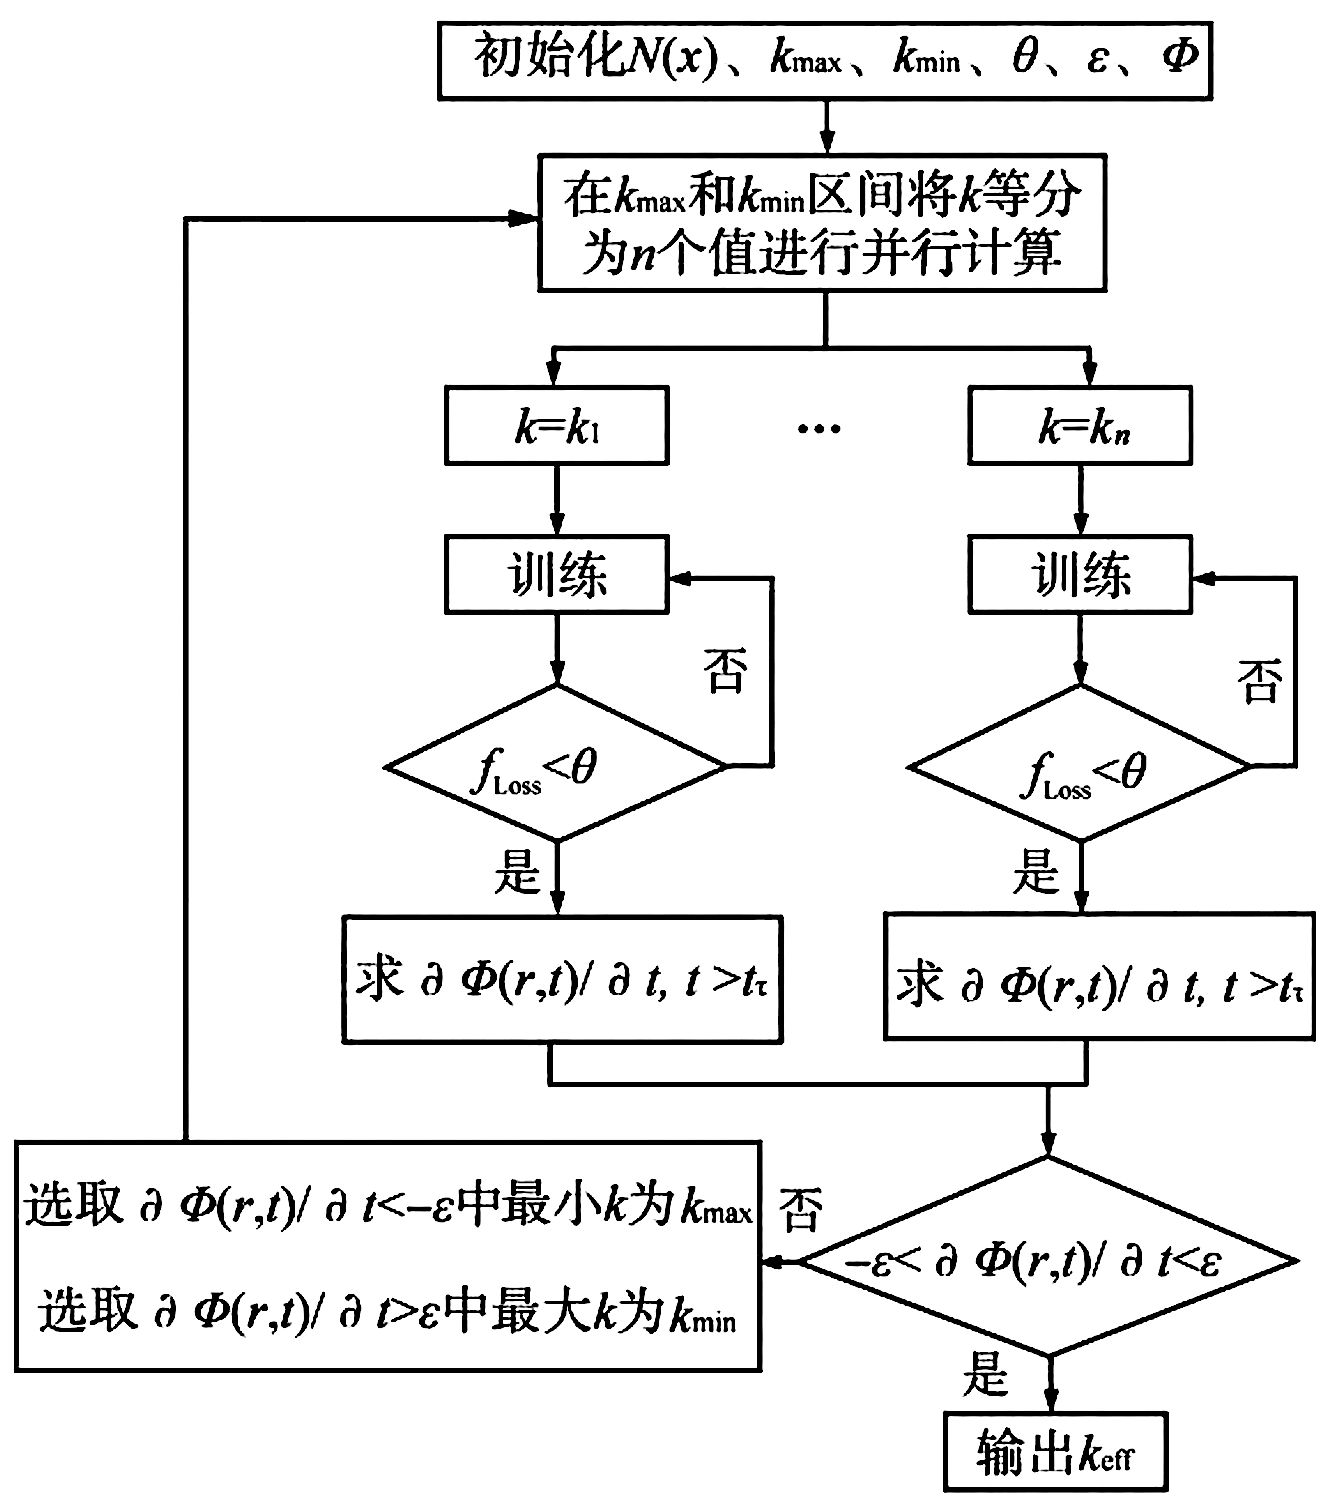
\includegraphics[width=0.5\textwidth]{./figure/k_eff并行搜索流程图.png} % 替换为你的图片文件名
    \cnenfigcaption{$k_{eff}$ 并行搜索流程图}{Flow chart of $k_{eff}$ parallel search}
    \label{fig:k_eff并行搜索流程图}
\end{figure}

本文采用式 \eqref{eq:单群扩散方程(lw)} 进行 $k_{\text {eff }}$ 的搜索, 将式 \eqref{eq:均匀裸堆稳态单群扩散方程(lw)} 写成式 \eqref{eq:单群扩散方程(lw)} 的形式:
\begin{equation}
    \frac{1}{D v} \frac{\partial \phi(r, t)}{\partial t}=\nabla^2 \phi(r, t)+\frac{k_{\infty} / k-1}{L^2} \phi(r, t)
\label{eq:单群扩散方程(lw)2}
\end{equation}

给出 $k$ 与 $\phi\left(r, t_0\right)$ 的任意初始值, 考察经过一定时间 $t_t$, 即 $t>t_\tau$ 时, $\phi(r, t)$ 对 $t$ 的偏导数是否接近 0 , 从而进行临界判断.
可设定合适的 $\varepsilon$, 若 $\partial \phi(r, t) / \partial t>\varepsilon$, 判断为超临界状态, 需要增大 $k$ 值;若 $\partial \phi(r, t) / \partial t<-\varepsilon$, 为次临界状态, 需要减小 $k$ 值.
当 $-\varepsilon<\partial \phi(r, t) / \partial t<\varepsilon$, 则认为系统已达临界, 此时 $k=k_{\mathrm{eff}}, \phi\left(r, t>t_{\mathrm{r}}\right)$ 即为稳态时系统的 $\phi(r)$ 分布 (式 \eqref{eq:均匀裸堆稳态单群扩散方程(lw)} ).

$t_\tau$ 的取值应大于注量率从任意初始状态到达 “稳定”变化状态的时间,根据扩散方程中反应堆类型[表现为式 \eqref{eq:单群扩散方程(lw)2} 中的 $Dv$ ]与初始边界条件形 式会有所不同;
$k$ 值的搜索方法可采用二分法或 者将 $k$ 等分成一定数量后,大规模并行搜索,可有效提高效率.$k_{eff}$ 的并行搜索流程如图 \ref{fig:k_eff并行搜索流程图} 所示.

\subsubsection{几何空间网格点密度不均匀分布策略}\label{sec:几何空间网格点密度不均匀分布策略}
式 \eqref{eq:多群中子学扩散方程模型}  $\sim$ 式 \eqref{eq:均匀裸堆稳态单群扩散方程(lw)} 中空间网格几何点 $i$ 的分布与数量, 对模型精度与机器学习效率的影响很大.通常来说, 网格点的数量越多, 计算精度越高,但计算量越大,收敛效率降低.同时,初始条件、边界条件及 $\phi(\vec{x})$ 变化很大的地方网格点密度对模型的精度与收敛效率影响很大.

为了平衡机器学习训练精度与效率, 推荐的策略是在相同网格点数量情况下, $\phi(\vec{x})$ 变化大的区域网格点相对紧密, 变化平滑的区域相对稀疏,以 $\phi(\vec{x})$ 在几何空间区域网格点偏导数的变化值作为网格点密度设定的判别依据.

据此,在方程的边界条件和初始条件附近,或者系统 $\phi(\vec{x})$ “畸性” 比较大处 ( 即区域偏导较大处 ), 应加密网格点提高精度, 而在变化平缓处 (即几何区域点偏导较小处),应减小网格密度以提高收敛效率.
\subsection{数值验证程序的复现}

为了便于计算和讨论,在本文中选择了结构相对简单的平板几何形式的扩散方程进行数值验证.这样的选择使得能够更清晰地理解和分析神经网络在特定几何条件下的性能,为进一步的讨论提供基础.

\subsubsection{深度机器学习的超参数设置}

为了验证计算结果,选择了具有解析解的特定几何形式的扩散方程进行数值验证.这些验证结果不仅对当前方程形式进行了验证,同时也为其他形式的方程和几何形状提供了参考.

以下是使用的神经网络的具体超参数设置,详见表 \ref{tab:hyperparameter_settings}:
\begin{table}[H]
    \caption{神经网络超参数及相关设置}
    \centering
    \begin{tabular}{ccc}
        \toprule
        \textbf{超参数} && \textbf{设置} \\
        \midrule
        \textbf{网络结构} &$\mathcal{N}(\vec{x})$& 全连接神经网络 \\
        \textbf{深度} &$l$& 16 \\
        \textbf{中间层神经元数量}  &$s$& 20 \\
        \textbf{激活函数} &$\sigma$& 双曲正切函数  $\tanh(x)=\frac{\mathrm{e}^x-\mathrm{e}^{-x}}{\mathrm{e}^x+\mathrm{e}^{-x}}$ \\
        \textbf{损失函数} &$Loss$& $Loss: M S E_u+M S E_{\{R, B C, I C\}}$ \\
        \textbf{边界权重}  &$P_{\mathrm{b}}$& 100 \\
        \textbf{学习率} &$lr$& 0.001  \\
        \textbf{优化器} && Adam  \\
        \textbf{网络初始化方法} && 高斯分布随机采样 \\
        \textbf{训练停止条件} && 达到设定的训练次数\\
        \bottomrule
    \end{tabular}
    \label{tab:hyperparameter_settings}
\end{table}
\subsubsection{临界条件下稳态扩散方程的验证}

选择了平板几何结构的扩散方程进行验证,该几何结构的解析解为$C\cdot\cos(x\cdot\pi/a)$,其中 $C=0.5$ 为常数,$a=1$ 为平板的长度.有关验证计算神经网络的超参数设置,请参见表 \ref{tab:hyperparameter_settings}.

在接下来的内容中,将逐步完成上述描述的扩散方程求解器的实现.作为示例,将使用 \texttt{Python} 语言和深度学习框架 \texttt{DeepXDE}\footnote{\texttt{DeepXDE} 是一个用于求解微分方程的 \texttt{Python} 包,其主要特点是使用深度学习技术求解微分方程,其官方网站为 \url{https://deepxde.readthedocs.io}.} 进行求解.具体的代码如下所示:

\noindent
首先,导入 \texttt{DeepXDE} 和 \texttt{numpy} 等必要的模块.
\begin{lstlisting}[style=python,basicstyle=\footnotesize\fontspec{Courier New},]  
    import deepxde as dde
    import numpy as np
    import os
    import matplotlib.pyplot as plt
\end{lstlisting}
初始化相关参数
\begin{lstlisting}[style=python,basicstyle=\footnotesize\fontspec{Courier New},]  
    # 初始化参数
    k_eff = 1  # 有效增殖系数
    a = 1  # 平板的宽度
    B2 = (np.pi / a) ** 2  # 系统临界时的几何曲率
    l = 16  # 神经网络的深度
    s = 20  # 神经网络的中间层隐藏神经单元数量
    Pb = 100  # 边界权重
    C = 0.5  # 解析解参数
\end{lstlisting}
定义解析解 $C\cdot\cos(x\cdot\pi/a)$
\begin{lstlisting}[style=python,basicstyle=\footnotesize\fontspec{Courier New},]  
    # 定义解析解
    def phi_analytical(x):
        return C * np.cos(x * np.pi / a)    
\end{lstlisting}
使用内置的 \texttt{Interval} 类定义一个几何求解区域 $[-a/2,a/2]$,如下所示:
\begin{lstlisting}[style=python,basicstyle=\footnotesize\fontspec{Courier New},]  
    # 定义几何网格
    geom = dde.geometry.Interval(-a / 2, a / 2)    
\end{lstlisting}
接下来,表达扩散方程\eqref{eq:均匀裸堆稳态单群扩散方程2(lw)}的 PDE 残差函数$\nabla^2 \phi(r)+B_g^2 \phi(r)$,如下所示:

\begin{lstlisting}[style=python,basicstyle=\footnotesize\fontspec{Courier New},]  
    # 定义微分方程
    def pde(x, phi):
        dphi_xx = dde.grad.hessian(phi, x, i=0, j=0)
        return dphi_xx + B2 * phi
\end{lstlisting}
\texttt{pde} 的第一个参数是网络输入,即横坐标.第二个参数是网络输出,即解,但这里使用$y$作为变量的名称.

接下来,考虑平板反应堆的外推边界条件 \eqref{eq:边界条件},即 $\phi(\pm\frac{a}{2})=0$.使用一个简单的 \texttt{Python} 函数,返回一个布尔值,
来定义平板反应堆的外推边界条件的子域$(\{-a/2,a/2\})$.该函数应该对子域内的点返回\texttt{True},对于外部的点返回\texttt{False}.
在的情况下,平板反应堆的外推边界条件的点 $x$ 是 $-a/2$ 和 $a/2$.
\begin{lstlisting}[style=python,basicstyle=\footnotesize\fontspec{Courier New},]  
    # 定义边界条件
    bc = dde.icbc.DirichletBC(geom, lambda x: 0, lambda _, on_boundary: on_boundary)
\end{lstlisting}
现在,已经指定了几何形状、扩散方程的 PDE 残差和外推边界条件.然后,定义PDE问题:
\begin{lstlisting}[style=python,basicstyle=\footnotesize\fontspec{Courier New},]  
    # 定义数据
    data = dde.data.PDE(geom, pde, bc, num_domain=898, num_boundary=2, solution=phi_analytical, num_test=100)
\end{lstlisting}
数字 \texttt{num\_domain=898} 是在域内采样的训练残差点的数量,数字 \texttt{num\_boundary=2} 是在边界上采样的训练点的数量.
参数 \texttt{solution=phi\_analytical} 是用于计算解的误差的参考解,如果没有参考解,可以忽略它.
使用 \texttt{num\_test=100} 个残差点来测试PDE残差.

接下来,选择网络.在这里,使用深度为 $l=16$(即 16 个隐藏层)宽度为 $s=20$ 的全连接神经网络, 其网络初始值权重采用高斯分布随机采样,并选用 $tanh$ 函数作为激活函数:
\begin{lstlisting}[style=python,basicstyle=\footnotesize\fontspec{Courier New},]  
    # 定义神经网络
    layer_size = [1] + [s] * l + [1]
    activation = "tanh"
    # 网络初始值权重采用高斯分布随机采样
    initializer = "Glorot uniform"
    net = dde.nn.PFNN(layer_size, activation, initializer)
\end{lstlisting}
现在,有了 PDE 问题和网络.下面构建一个 Model,并选择 Adam 作为优化器和初始学习率 \texttt{lr=0.001}:
\begin{lstlisting}[style=python,basicstyle=\footnotesize\fontspec{Courier New},]  
    # 定义模型
    model = dde.Model(data, net)
    # 定义求解器
    model.compile("adam", lr=0.001, metrics=["l2 relative error"], loss_weights=[1, Pb])
\end{lstlisting}
这里通过 \texttt{loss\_weights=[1, Pb]} 将边界处的损失权重调整为 $100$, 同时还选用 \texttt{metrics=["l2 relative error"]} 计算在测试点上训练好的神经网络输出与对应解析解的 $L_2$ 相对误差作为训练过程中的一个指标.
然后,对模型进行 3500 次迭代训练, 并使用 \texttt{dde.saveplot} 回调函数在训练期间保存模型和图片, 最后输出在 $x=0$ 处的值(即 C), 以此来显示特征值方程解(特征向量)的不确定性.
\begin{lstlisting}[style=python,basicstyle=\footnotesize\fontspec{Courier New},]  
    # 训练模型
    losshistory, train_state = model.train(epochs=3500)
    # 保存和可视化训练结果
    dde.saveplot(losshistory, train_state, issave=True, isplot=True)

    # 输出在 x=0 处的值(即 C)
    print("Predicted value at x=0:", model.predict(np.array([0])))
\end{lstlisting}

为了深入了解模型的训练过程、监控关键指标的变化,并直观地呈现训练效果,采用了以下可视化策略:

\noindent 创建保存图像的文件夹
\begin{lstlisting}[style=python,basicstyle=\footnotesize\fontspec{Courier New},]  
    output_folder = "figure/算例1"
    os.makedirs(output_folder, exist_ok=True)
\end{lstlisting}
设置中文字体
\begin{lstlisting}[style=python,basicstyle=\footnotesize\fontspec{Courier New},]  
    
    # 替换为您的字体文件路径
    font_path = '/System/Library/Fonts/STHeiti Light.ttc'
    
    # 添加字体路径
    font_properties = FontProperties(fname=font_path)
    plt.rcParams['font.sans-serif'] = [font_properties.get_name()]
    plt.rcParams['axes.unicode_minus'] = False
\end{lstlisting}  
绘制损失函数变化图
\begin{lstlisting}[style=python,basicstyle=\footnotesize\fontspec{Courier New},]  
    loss_train = np.sum(losshistory.loss_train, axis=1)
    loss_test = np.sum(losshistory.loss_test, axis=1)
    
    plt.figure(figsize=(6, 5))  # 设置图像大小
    plt.semilogy(losshistory.steps, loss_train, label="训练损失")
    plt.semilogy(losshistory.steps, loss_test, label="测试损失")
    for i in range(len(losshistory.metrics_test[0])):
        plt.semilogy(
            losshistory.steps,
            np.array(losshistory.metrics_test)[:, i],
            label="测试指标",
        )
    plt.xlabel("步骤")
    plt.legend()
    # 保存为png
    plt.tight_layout()
    plt.savefig(os.path.join(output_folder, "losshistory.png"), format="png", dpi=200)
\end{lstlisting}  
绘制训练状态变化图
\begin{lstlisting}[style=python,basicstyle=\footnotesize\fontspec{Courier New},]     
    def _pack_data(train_state):
        def merge_values(values):
            if values is None:
                return None
            return np.hstack(values) if isinstance(values, (list, tuple)) else values
    
        y_train = merge_values(train_state.y_train)
        y_test = merge_values(train_state.y_test)
        best_y = merge_values(train_state.best_y)
        best_ystd = merge_values(train_state.best_ystd)
        return y_train, y_test, best_y, best_ystd
    
    
    if isinstance(train_state.X_train, (list, tuple)):
        print(
            "错误:网络有多个输入,尚未实现绘制此类结果."
        )
    
    y_train, y_test, best_y, best_ystd = _pack_data(train_state)
    y_dim = best_y.shape[1]
\end{lstlisting}  
回归分析图
\begin{lstlisting}[style=python,basicstyle=\footnotesize\fontspec{Courier New},]         
    if train_state.X_test.shape[1] == 1:
        idx = np.argsort(train_state.X_test[:, 0])
        X = train_state.X_test[idx, 0]
        plt.figure(figsize=(6, 5))  # 设置图像大小
        for i in range(y_dim):
            if y_train is not None:
                plt.plot(train_state.X_train[:, 0], y_train[:, i], "ok", label="训练点分布")
            if y_test is not None:
                plt.plot(X, y_test[idx, i], "-k", label="真实")
            plt.plot(X, best_y[idx, i], "--r", label="预测")
            if best_ystd is not None:
                plt.plot(
                    X, best_y[idx, i] + 2 * best_ystd[idx, i], "-b", label="95% 置信区间"
                )
                plt.plot(X, best_y[idx, i] - 2 * best_ystd[idx, i], "-b")
        plt.xlabel("x")
        plt.ylabel("y")
        plt.legend()
        plt.savefig(os.path.join(output_folder, "solution_state.png"), format="png", dpi=200)
\end{lstlisting}  
神经网络输出的残差
\begin{lstlisting}[style=python,basicstyle=\footnotesize\fontspec{Courier New},]  
    if y_test is not None:
        plt.figure(figsize=(6, 5))  # 设置图像大小
        residual = y_test[:, 0] - best_y[:, 0]
        plt.plot(best_y[:, 0], residual, "o", zorder=1)
        plt.hlines(0, plt.xlim()[0], plt.xlim()[1], linestyles="dashed", zorder=2)
        plt.xlabel("预测值")
        plt.ylabel("残差 = 观测 - 预测")
        plt.tight_layout()
        plt.savefig(os.path.join(output_folder, "y_test.png"), format="png", dpi=200)
\end{lstlisting}  
神经网络输出的标准差
\begin{lstlisting}[style=python,basicstyle=\footnotesize\fontspec{Courier New},]
    if best_ystd is not None:
        plt.figure(figsize=(6, 5))  # 设置图像大小
        for i in range(y_dim):
            plt.plot(train_state.X_test[:, 0], best_ystd[:, i], "-b")
            plt.plot(
                train_state.X_train[:, 0],
                np.interp(
                    train_state.X_train[:, 0], train_state.X_test[:, 0], best_ystd[:, i]
                ),
                "ok",
            )
        plt.xlabel("x")
        plt.ylabel("std(y)")
        plt.tight_layout()
        plt.savefig(os.path.join(output_folder, "best_ystd.png"), format="png", dpi=200)
\end{lstlisting}  
绘制数值解与解析解的图像并比较误差
\begin{lstlisting}[style=python,basicstyle=\footnotesize\fontspec{Courier New},]
    x = np.linspace(-a / 2, a / 2, 100).reshape((-1, 1))
    y_pred = model.predict(x)
    y_exact = phi_analytical(x)
    
    plt.figure(figsize=(12, 5))
    plt.subplot(1, 2, 1)
    plt.plot(x, y_pred, label="神经网络解", color="tab:blue")
    plt.plot(x, y_exact, label="解析解", color="tab:orange")
    plt.title("数值解与解析解的比较")
    plt.xlabel("x")
    plt.ylabel("$\phi(x)$")
    plt.legend()
    
    plt.subplot(1, 2, 2)
    plt.plot(x, np.abs(y_pred - y_exact), label="绝对误差", color="tab:red")
    plt.title("数值解与解析解的绝对误差")
    plt.xlabel("x")
    plt.ylabel("绝对误差")
    plt.legend()
    
    plt.tight_layout()
    plt.savefig(os.path.join(output_folder, "solution_comparison.png"), format="png", dpi=200)
    
    plt.show()
\end{lstlisting}
通过深度学习网络训练的结果进行可视化展示,包括训练过程中的损失函数变化和最终效果.首先,关注损失函数变化图,如图~\ref{fig:losshistory} 所示.图中横轴表示训练步骤,纵轴表示误差数量级,分别展示了训练损失和测试损失的变化情况.从图中可以清晰地观察到,随着训练的进行,训练损失逐渐降低,而测试损失也呈现下降趋势,这表明网络在学习过程中取得了良好的效果.

此外,图中还展示了测试阶段的指标(数值解与解析解比较)变化.图中显示,随着训练的进行,测试指标几乎保持稳定,且其值相对较大,这表明数值解与解析解始终保持较大误差.这为提供了对网络性能的更全面认识.

\begin{figure}[H]
    \centering
    \begin{minipage}[c]{0.48\textwidth}
    \centering
    \includegraphics[width=0.8\textwidth]{./figure/算例1/losshistory.png}
    \end{minipage}
    \hspace{0.02\textwidth}
    \begin{minipage}[c]{0.48\textwidth}
    \centering
    \includegraphics[width=0.8\textwidth]{./figure/算例2/losshistory.png}
    \end{minipage}\\[3mm]
    \begin{minipage}[t]{0.48\textwidth}
    \centering
    \cnenfigcaption{损失函数变化图}{Loss function change}
    \label{fig:losshistory}
    \end{minipage}
    \hspace{0.02\textwidth}
    \begin{minipage}[t]{0.48\textwidth}
    \centering
    \cnenfigcaption{优化后损失函数变化图}{Loss function change after optimization}
    \label{fig:losshistory2}
    \end{minipage}
    \end{figure}

    接下来,关注回归分析图,图~\ref{fig:Regression analysis} 展示了神经网络训练点的采样分布情况、真实数据的曲线以及网络的预测曲线.从图中可以看出,网络预测曲线与真实曲线趋势相差很大.
\begin{figure}[H]
    \centering
    \begin{minipage}[c]{0.48\textwidth}
    \centering
    \includegraphics[width=0.8\textwidth]{./figure/算例1/solution_state.png}
    \end{minipage}
    \hspace{0.02\textwidth}
    \begin{minipage}[c]{0.48\textwidth}
    \centering
    \includegraphics[width=0.8\textwidth]{./figure/算例2/solution_state.png}
    \end{minipage}\\[3mm]
    \begin{minipage}[t]{0.48\textwidth}
    \centering
    \cnenfigcaption{回归分析图}{Regression analysis}
    \label{fig:Regression analysis}
    \end{minipage}
    \hspace{0.02\textwidth}
    \begin{minipage}[t]{0.48\textwidth}
    \centering
    \cnenfigcaption{优化后回归分析图}{Regression analysis after optimization}
    \label{fig:Regression analysis2}
    \end{minipage}
    \end{figure}
    另外,通过图~\ref{fig:Residual analysis} 进行的针对测试数据的残差分析显示,残差的分布情况较为随机,且残差的绝对值相对较大,这表明网络的预测效果并不理想.这一现象可以部分归因于特征值方程的特征向量存在不确定性,导致收敛得到的特征向量是不同的(表现为收敛时 $C$ 值不同),且很难取得一致的收敛结果.

    此外,注意到通过神经网络的输出值几乎全为$0$,这表明神经网络可能倾向于选择一个近似为 $0$ 的解.这种行为符合神经网络在学习过程中对低频解的优先偏好.
\begin{figure}[H]
    \centering
    \begin{minipage}[c]{0.48\textwidth}
    \centering
    \includegraphics[width=0.8\textwidth]{./figure/算例1/y_test.png}
    \end{minipage}
    \hspace{0.02\textwidth}
    \begin{minipage}[c]{0.48\textwidth}
    \centering
    \includegraphics[width=0.8\textwidth]{./figure/算例2/y_test.png}
    \end{minipage}\\[3mm]
    \begin{minipage}[t]{0.48\textwidth}
    \centering
    \cnenfigcaption{残差分析图}{Regression analysis}
    \label{fig:Residual analysis}
    \end{minipage}
    \hspace{0.02\textwidth}
    \begin{minipage}[t]{0.48\textwidth}
    \centering
    \cnenfigcaption{优化后残差分析图}{Regression analysis after optimization}
    \label{fig:Residual analysis2}
    \end{minipage}
    \end{figure}

    为了解决上述问题,采用了 \ref{sec:扩散方程特征向量加速收敛方法} 节中提到的改进方法,具体而言,将扩散方程的特殊空间点、多个区域平均值/积分值与预设值的均方差作为额外的加权因素,并采用类似于初始条件、边界条件的处理方法进行加权处理.相关代码段如下:
\begin{lstlisting}[style=python,basicstyle=\footnotesize\fontspec{Courier New},]  
    # 扩散方程特征向量加速收敛方法验证
    observe_x = np.array([0])
    observe_phi0 = dde.icbc.PointSetBC(observe_x, phi_analytical(observe_x))
    # 定义数据
    data = dde.data.PDE(geom, pde, [bc,observe_phi0], num_domain=898, num_boundary=2, anchors=observe_x, solution=phi_analytical, num_test=100)
\end{lstlisting}
首先,聚焦于添加了额外加权因素的损失函数变化图,如图~\ref{fig:losshistory2} 所示.从图中清晰可见,随着训练的进行,三种损失均呈现下降趋势,这表明网络在学习过程中取得了良好的效果.

接着,研究回归分析图~\ref{fig:Regression analysis2} 以及测试数据的残差分析图~\ref{fig:Residual analysis2},从图中可以看出,预测曲线与真实曲线趋势相符.

此外,注意到如图~\ref{fig:Residual analysis2} 所示,预测曲线与真实曲线在边界处的残差很大.这表明直接使用经典 PINN 对边界条件进行约束的方法并不理想,因此考虑采用硬边界约束的方法进行改进.

具体做法是定义神经网络输出的转换:
\begin{equation}
    \phi(\vec{x})=\vec{x} \cdot(\pi-\vec{x}) \cdot y+\vec{x}
\end{equation}
并将其应用于网络.当 $\vec{x}=\pm \frac{a}{2}$ 时,边界条件 $\phi(\pm \frac{a}{2})=0$ 得到满足.这表明边界约束的两端都是硬条件.相关代码段如下所示:

\begin{lstlisting}[style=python,basicstyle=\footnotesize\fontspec{Courier New},]  
    # 定义硬边界条件
    def output_transform(x, y):
        return (x + a / 2) * (x - a / 2) * y
    net.apply_output_transform(output_transform)
\end{lstlisting}

在这段代码中,定义了一个名为 \texttt{output\_transform} 的函数,它对输出进行了转换.具体而言,对于给定的输入 \texttt{x} 和输出 \texttt{y},转换后的输出是 $\vec{x} \cdot (\pi - \vec{x}) \cdot y + \vec{x}$.

然后,通过 \texttt{net.apply\_output\_transform(output\_transform)} 将这个输出转换函数应用于网络.这表示通过这个转换函数考虑了边界条件的硬约束,确保网络的输出满足问题的物理边界条件.

最后,再次研究回归分析图~\ref{fig:Regression analysis3} 以及测试数据的残差分析图~\ref{fig:Residual analysis3},从图中可以看出,预测曲线与真实曲线趋势相符,残差的绝对值较小,且在边界处误差为 $0$.这表明采用硬边界条件的网络的预测效果最佳.实验证明在本文的其他算例中也存在类似的现象,因此将在后续的算例中继续采用硬边界条件的网络进行计算.
\begin{figure}[H]
    \centering
    \begin{minipage}[c]{0.48\textwidth}
    \centering
    \includegraphics[width=0.8\textwidth]{./figure/算例2/硬边界/solution_state.png}
    \end{minipage}
    \hspace{0.02\textwidth}
    \begin{minipage}[c]{0.48\textwidth}
    \centering
    \includegraphics[width=0.8\textwidth]{./figure/算例2/硬边界/y_test.png}
    \end{minipage}\\[3mm]
    \begin{minipage}[t]{0.48\textwidth}
    \centering
    \cnenfigcaption{硬边界条件回归分析图}{Regression analysis with hard BC}
    \label{fig:Regression analysis3}
    \end{minipage}
    \hspace{0.02\textwidth}
    \begin{minipage}[t]{0.48\textwidth}
    \centering
    \cnenfigcaption{硬边界条件残差分析图}{Residual analysis with hard BC}
    \label{fig:Residual analysis3}
    \end{minipage}
    \end{figure}
    

% 具体求解结果如表 \ref{tab:verification_results} 所示.

% \begin{table}[H]
%     \centering
%     \begin{tabular}{ccccccc}
%         \toprule
%         \textbf{类型} & \textbf{网格点 $(i)$} & \textbf{学习次数 $(n)$} & \textbf{几何参数 $/ \mathrm{m}$} & $\sigma_{\mathrm{MSE}, 1}$ & $\sigma_{\mathrm{SE}, \mathrm{max}}$ & $\sigma_{\mathrm{MSE}, \mathrm{mc}}$ \\
%         \midrule
%         平板 & 900 & 3500 & $a=1$ & $1.4850 \times 10^{-9}$ & $4.9266 \times 10^{-9}$ & $4.8897 \times 10^{-6}$ \\
%         \bottomrule
%     \end{tabular}
%     \caption{临界条件下稳态扩散方程验证结果}
%     \label{tab:verification_results}
% \end{table}

% $\sigma_{\mathrm{MSE}, 1}$ 为学习好的神经网络函数 $\mathcal{N}(\vec{x})$ 在所有网格点上泛化计算结果与解析解的均方差; $\sigma_{\mathrm{SE} i \text { max }}$ 是网格点集合中每个点处的 $\mathcal{N}(\vec{x})$ 与解析解的方差最大值; $\sigma_{\mathrm{MSE}, \mathrm{mc}}$ 是蒙特卡洛方法软件 RMC 计算结果与解析解均方差.

% 从结果可知,整体上机器学习模型具有相当高的精度.然而,随着扩散方程的输入维度和复杂程度增加,系统的精度略有降低.模型与解析解的均方差分布具有一定程度的随机性,存在个别误差较高的畸点.这些现象部分归因于深度神经网络本身的不可解释性特性.同时,在计算效率方面,虽然整体训练时间通常大于传统数值计算方法,但在训练完成后,神经网络进行预测的时间极短,几乎可以忽略不计.

\subsubsection{验证扩散方程特征向量加速收敛方法}

为验证扩散方程特征向量加速收敛方法的有效性,选择了平板几何结构的扩散方程进行验证.该几何结构的解析解为$C\cdot\cos(x\cdot\pi/a)$,其中 $C=0.5$ 为常数,$a$ 为平板的长度.验证计算神经网络的超参数设置见表 \ref{tab:hyperparameter_settings}.

\noindent 以下是加速收敛的代码段:
\begin{lstlisting}[style=python,basicstyle=\footnotesize\fontspec{Courier New},]  
    # 扩散方程特征向量加速收敛方法验证
    observe_x = np.array([0])
    observe_phi0 = dde.icbc.PointSetBC(observe_x, phi_analytical(observe_x))
    # 定义数据
    data = dde.data.PDE(geom, pde, [bc,observe_phi0], num_domain=898, num_boundary=2, anchors=observe_x, solution=phi_analytical, num_test=100)
\end{lstlisting}
验证计算的目标是统计并分析不同初始权重值 ${\vec{w}, \vec{b}}$ 的神经网络 $\mathcal{N}(\vec{x})$ 在训练相同次数时模型所达到的精度.

在算例 1 和算例 2 中,网络初始值权重 ${\vec{w}, \vec{b}}$ 被随机选择.在算例 3 中,同样选择随机初始值,但将 $x=0$ 时的 $\phi(0)$ 值设定为解析解中的 $C$ 值,即0.5.在算例 4、算例 5、算例 6、算例 7 中,初始状态为具有不同 $C_0$ 值且已经事先训练好的精度小于 $10^{-3}$ 的网络.训练方式与算例 3 类似,将 $\phi(0)=0.5$ 作为加权损失函数的组成部分进行训练.各算例均训练1000次即停止,记录精度及学习完成时的 $C$ 值等相关参数,结果如表 \ref{tab:sensitivity_analysis_results} 所示.
\begin{table}[H]
    \caption{神经网络初始值敏感性分析结果}
    \centering
    \begin{tabular}{cccccc}
        \toprule
        \textbf{算例} & \textbf{网络初始值 $/ C_0$ 值} & \textbf{目标 $C$ 值设定} & 残差 & \textbf{学习次数 $(n)$} & \textbf{学习完成时 $C$ 值} \\
        \midrule
        1 & 随机/随机 & 无 &  & 1000 & 0.000000 \\
        2 & 随机/随机 & 无 &  & 1000 & 0.000000 \\
        3 & 随机/随机 & 0.5 & $1.96e-04$ & 1000 & 0.499856 \\
        4 & 已训练 $/ C_0=0.01$ & 0.5 & $9.87e-05$ & 1000 & 0.499986 \\
        5 & 已训练 $/ C_0=0.05$ & 0.5 & $5.37e-05$ & 1000 & 0.499994 \\
        6 & 已训练 $/ C_0=0.1$ & 0.5 & $2.52e-05$ & 1000 & 0.499999 \\
        7 & 已训练 $/ C_0=0.5$ & 0.5 & $6.90e-06$ & 1000 & 0.500000 \\
        \bottomrule
    \end{tabular}
    \label{tab:sensitivity_analysis_results}
\end{table}
% \begin{table}[H]
%     \centering
%     \begin{tabular}{cccccc}
%         \toprule
%         \textbf{算例} & \textbf{网络初始值 $/ C_0$ 值} & \textbf{目标 $C$ 值设定} & $\sigma_{\mathrm{MSE}, 1} / 10^{-8}$ & \textbf{学习次数 $(n)$} & \textbf{学习完成时 $C$ 值} \\
%         \midrule
%         1 & 随机/随机 & 无 & 9.9998 & 2405 & 0.015 \\
%         2 & 随机/随机 & 无 & 9.1095 & 1606 & 0.0022 \\
%         3 & 随机/随机 & 0.5 & 9.6124 & 379 & 0.4995 \\
%         4 & 已训练 $/ C_0=0.01$ & 0.5 & 9.1010 & 211 & 0.4996 \\
%         5 & 已训练 $/ C_0=0.05$ & 0.5 & 9.3309 & 55 & 0.4996 \\
%         6 & 已训练 $/ C_0=0.1$ & 0.5 & 9.5475 & 39 & 0.4995 \\
%         \bottomrule
%     \end{tabular}
%     \caption{神经网络初始值敏感性分析结果}
%     \label{tab:sensitivity_analysis_results}
% \end{table}
可见,算例 1 和算例 2 均收敛到 $C=0$,这说明了若不给定目标 $C$ 值作为训练的加权 $Loss$,由于特征值方程的特征向量不确定性,收敛得到的特征向量符合神经网络优先偏好学习低频解的特性.

在算例 3 中,由于设定了目标 $C$ 值,能够收敛到正确的解空间.而算例 4、算例 5、算例 6、算例 7 由于有预训练初始值,最终模型精度进一步提高.此外,初始 $C$ 值越接近目标值 $C=0.5$,精度越高.特别地,当初始 $C=0.5$ 时,其学习完成时的 $C$ 将完全等于目标值.这表明采用已训练好的神经网络作为相似问题神经网络初始值具有良好的迁移学习特性,可大幅度加快收敛进程.

\subsubsection{瞬态条件扩散方程求解及$k_{\text{eff}}$搜索方法验证}

根据 \ref{sec:均匀裸堆的单群扩散方程的解} 节中的讨论,瞬态方程式 (2) 在平板几何真空边界条件下解析解为:
\begin{equation}
\begin{aligned}
\phi(x, t)= & \sum_{n=1}^{\infty} \frac{2}{a}\left[\int_{-a / 2}^{a / 2} \phi_0\left(x^{\prime}\right) \cos \frac{(2 n-1) \pi}{a} x^{\prime} \mathrm{d} x^{\prime}\right] \times \\
& \cos \frac{(2 n-1) \pi}{a} x \mathrm{e}^{\left(k_n-1\right) t / l_n}
\end{aligned}\label{eq:瞬态扩散方程解析解10}
\end{equation}
其中
\begin{align}
l_n&=\frac{L^2}{Dv\left(1+L^2 B_n^2\right)}=\frac{l_{\infty}}{1+L^2 B_n^2}\\
k_n&=\frac{k_{\infty}}{1+L^2 B_n^2}\\
B_n&=\frac{(2 n-1) \pi}{a} \quad n=1,2,3, \cdots
\end{align}

\noindent 解析解计算代码段:
\begin{lstlisting}[style=python,basicstyle=\footnotesize\fontspec{Courier New},]  
    # 模型方程的参数
    v = 2.2e3  # m/s
    D = 0.211e-2  # m
    L_square = 2.1037e-4  # m^2
    a = 1  # m
    k_infinity = 1.0041

    # 初始条件
    def phi_0(x):
        return np.cos(np.pi * x / a) - 0.4 * np.cos(2 * np.pi * x / a) - 0.4
    
    # 解析解的计算
    def phi(x, t):
        summation = 0
        B_n = lambda n: (2 * n - 1) * np.pi / a
        for n in range(1, 10):  # 选择一个足够大的上限来近似无穷级数
            l_n = L_square / (D * v * (1 + L_square * B_n(n) ** 2))
            k_n = k_infinity / (1 + L_square * B_n(n) ** 2)
    
            integrand = lambda x_prime: phi_0(x_prime) * np.cos(B_n(n) * x_prime)
            integral_result, _ = quad(integrand, -a / 2, a / 2)
            summation += (2 / a) * integral_result * np.cos(B_n(n) * x) * np.exp((k_n - 1) * t / l_n)
    
        return summation
\end{lstlisting}
\begin{figure}[H]
    \centering
    \begin{minipage}[c]{0.48\textwidth}
    \centering
    
\includegraphics[width=\textwidth]{./figure/算例3/AnalyticalSolution1.png}
    \end{minipage}
    \hspace{0.02\textwidth}
    \begin{minipage}[c]{0.48\textwidth}
    \centering
    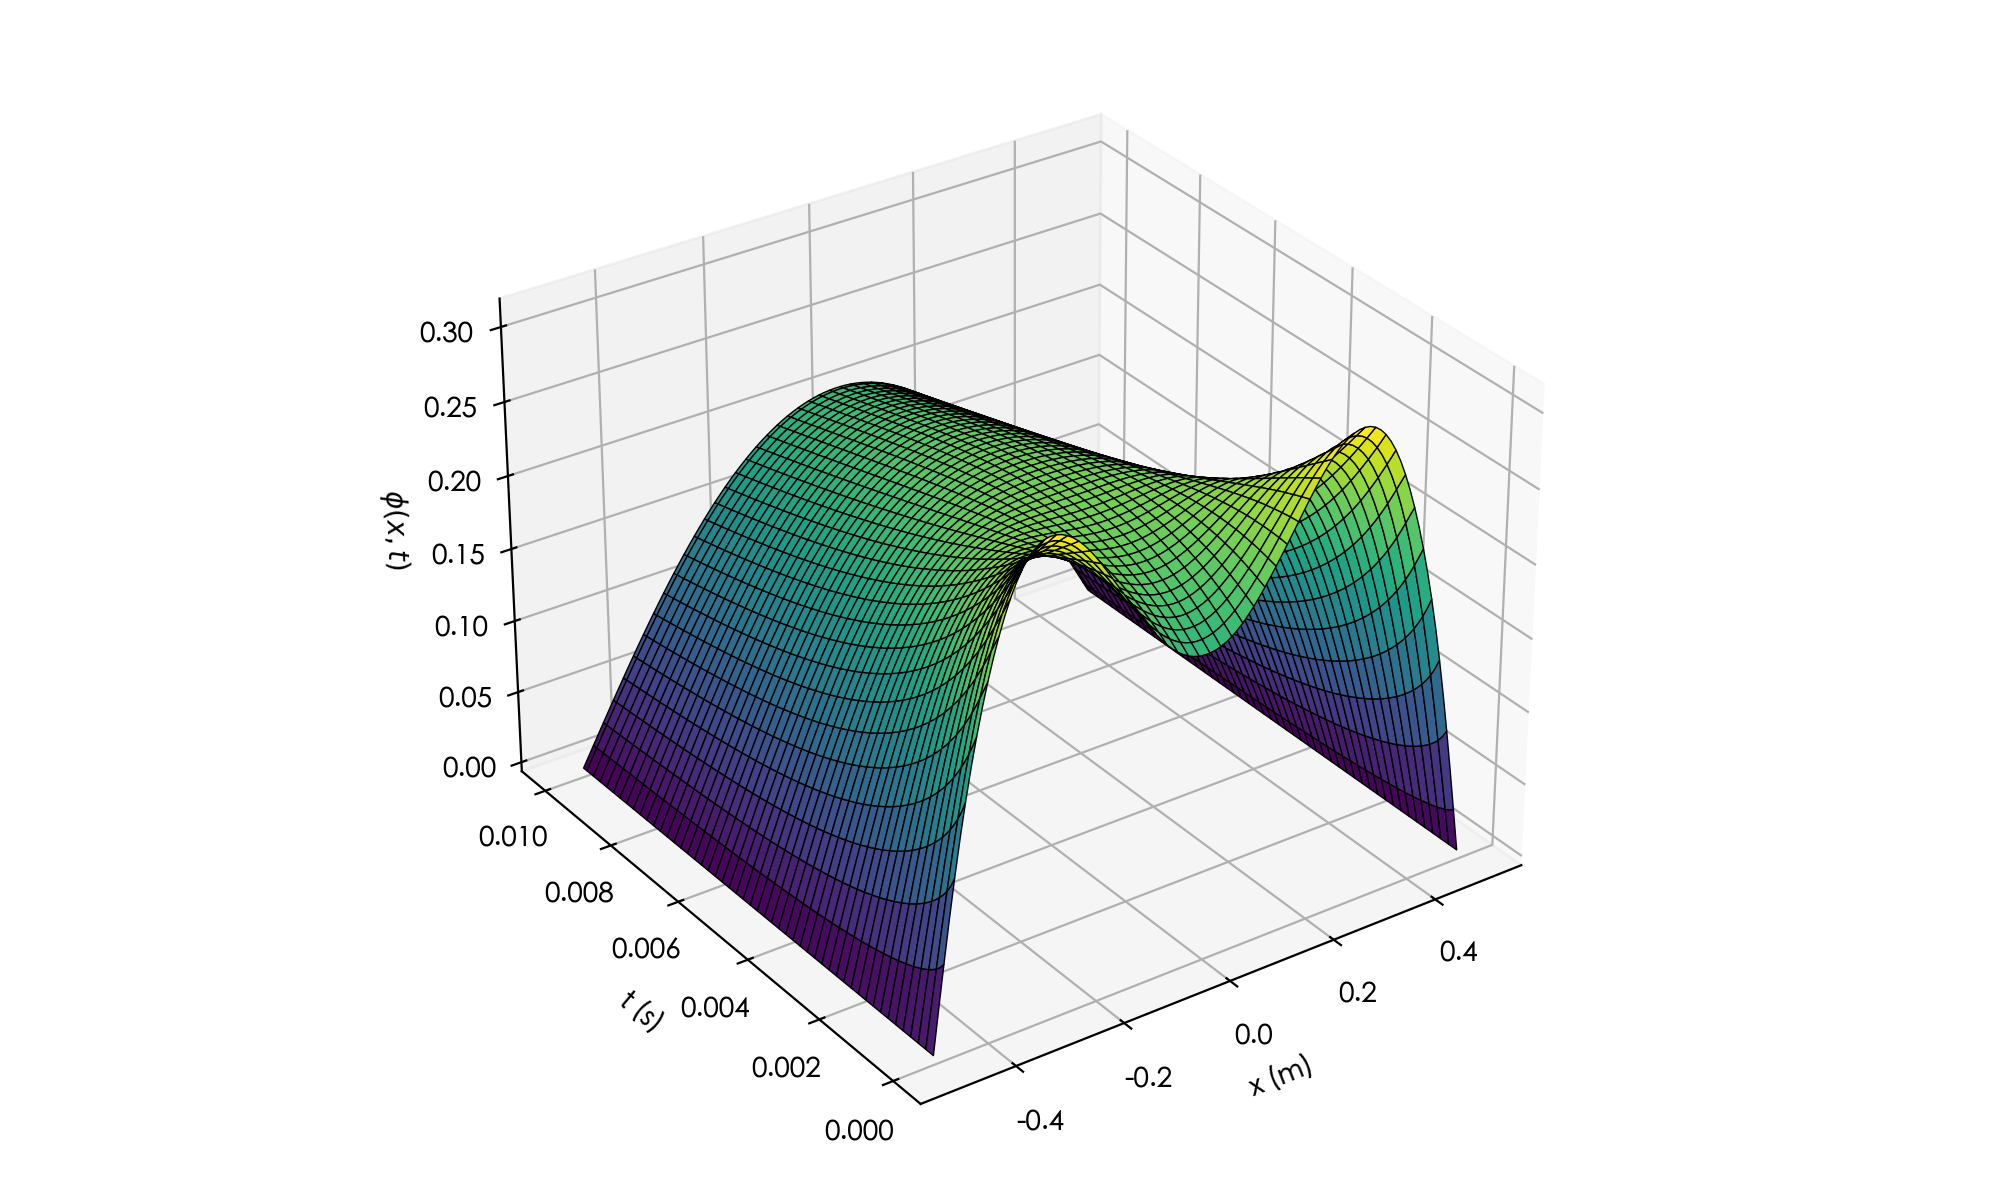
\includegraphics[width=\textwidth]{./figure/算例3/AnalyticalSolution2.png}
    \end{minipage}\\[3mm]
    \begin{minipage}[t]{0.48\textwidth}
    \centering
    \cnenfigcaption{算例1解析解}{Analytical solution of case 1}
    \label{fig:算例1解析解}
    \end{minipage}
    \hspace{0.02\textwidth}
    \begin{minipage}[t]{0.48\textwidth}
    \centering
    \cnenfigcaption{算例2解析解}{Analytical solution of case 2}
    \label{fig:算例2解析解}
    \end{minipage}
    \centering
    \begin{minipage}[c]{0.48\textwidth}
    \centering
    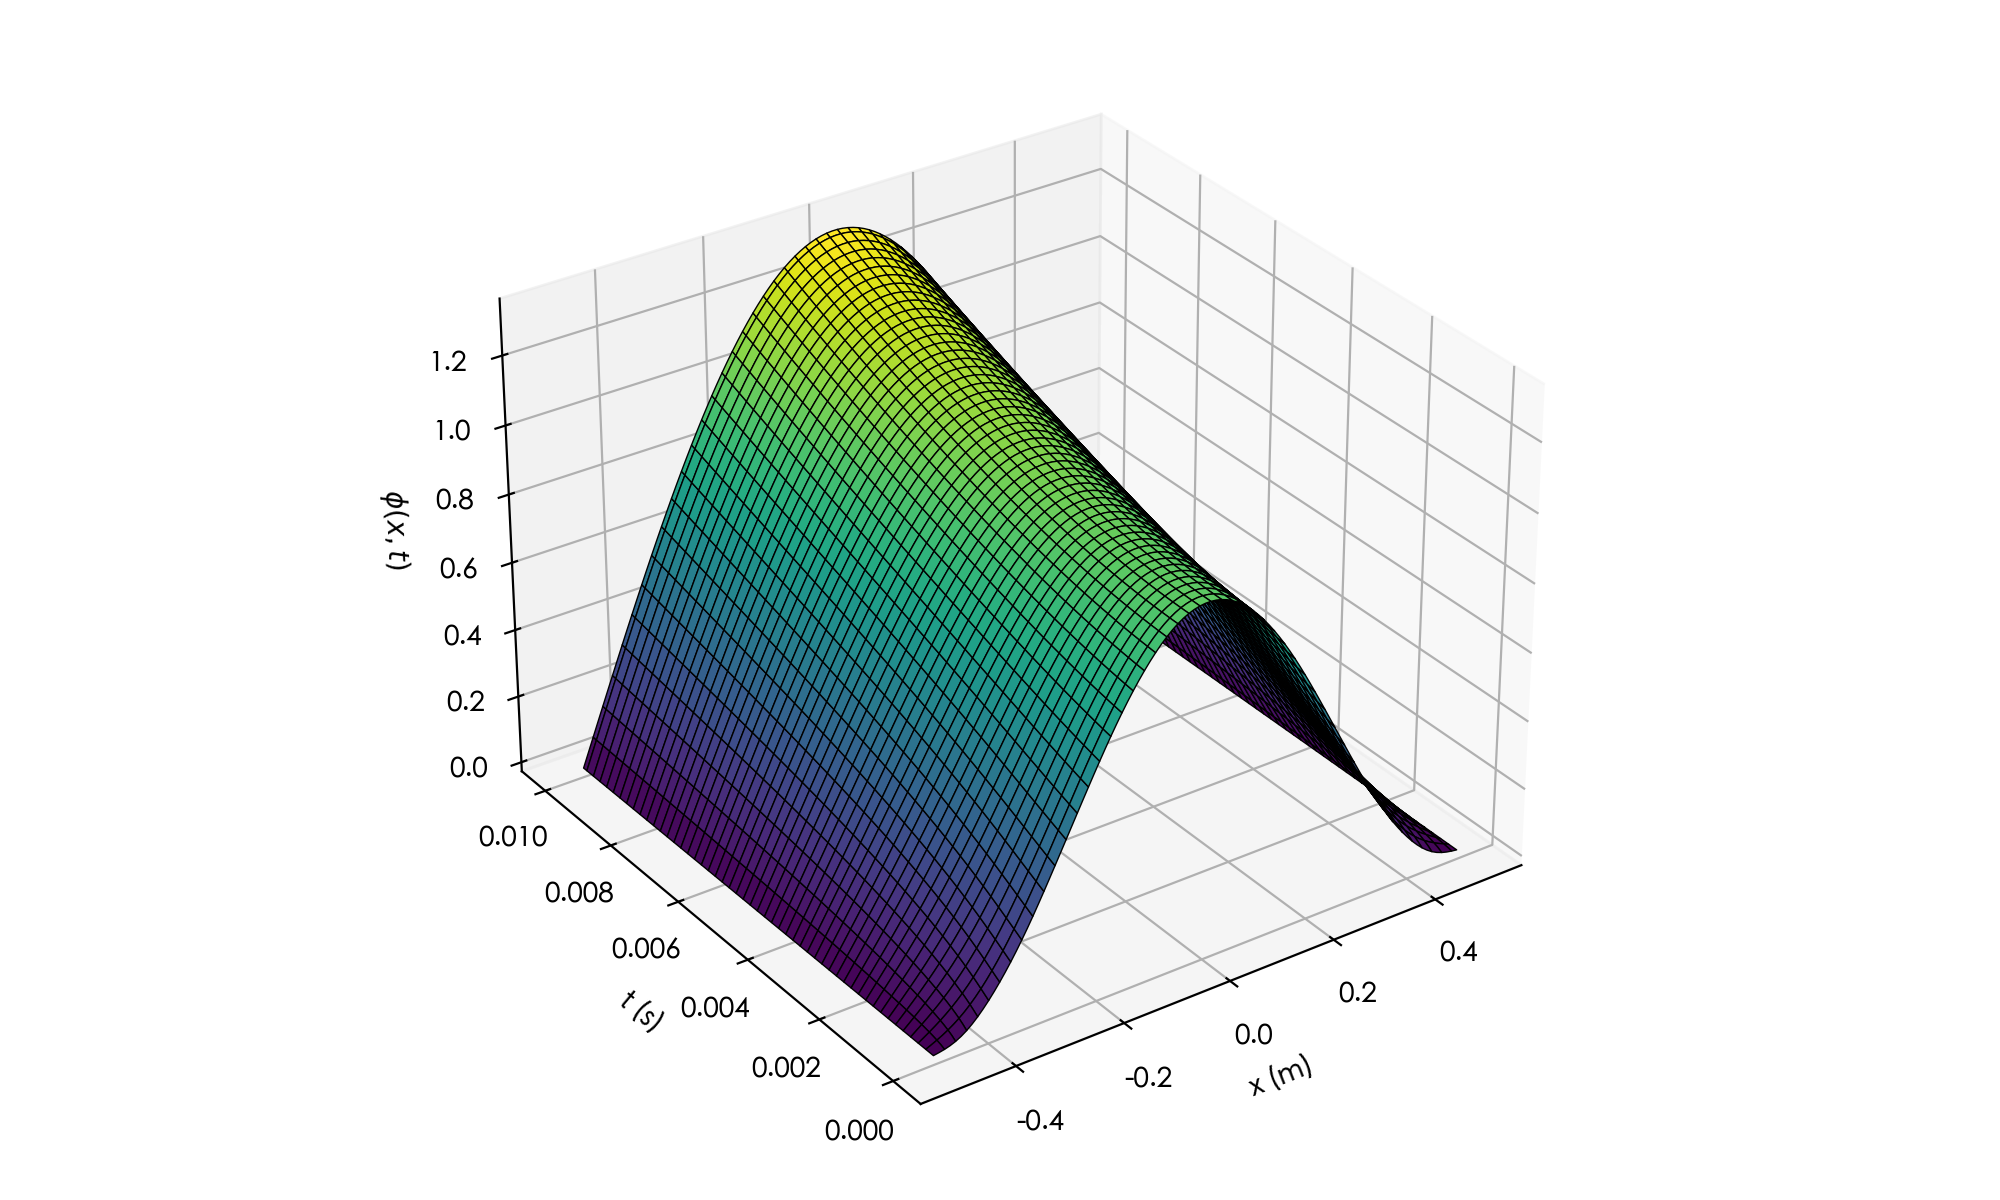
\includegraphics[width=\textwidth]{./figure/算例3/AnalyticalSolution3.png}
    \end{minipage}
    \hspace{0.02\textwidth}
    \begin{minipage}[c]{0.48\textwidth}
    \centering
    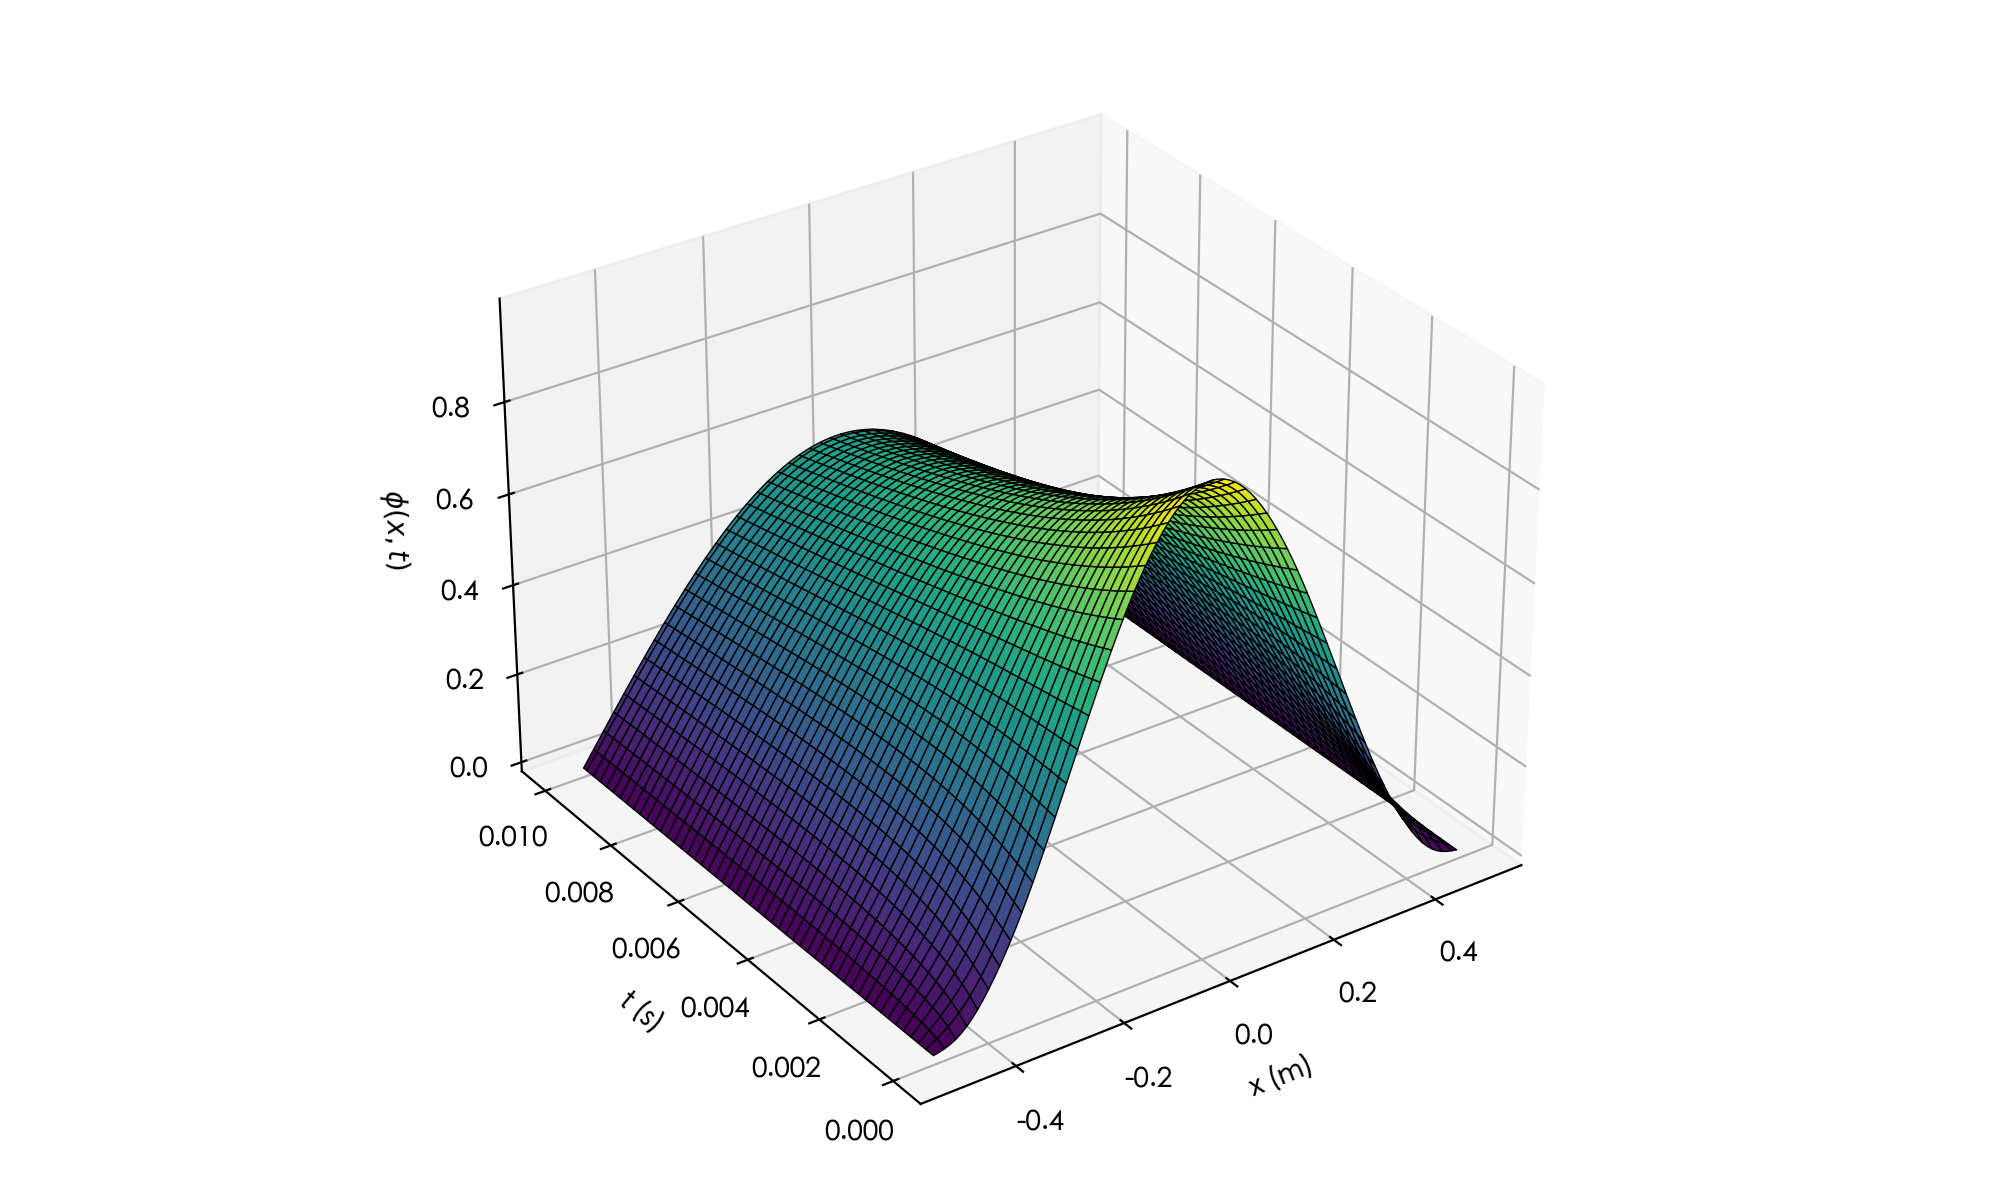
\includegraphics[width=\textwidth]{./figure/算例3/AnalyticalSolution4.png}
    \end{minipage}\\[3mm]
    \begin{minipage}[t]{0.48\textwidth}
    \centering
    \cnenfigcaption{算例3解析解}{Analytical solution of case 3}
    \label{fig:算例3解析解}
    \end{minipage}
    \hspace{0.02\textwidth}
    \begin{minipage}[t]{0.48\textwidth}
    \centering
    \cnenfigcaption{算例4解析解}{Analytical solution of case 4}
    \label{fig:算例4解析解}
    \end{minipage}
    \end{figure}
    
验证模型方程参数: $v=2.2 \times 10^3 \mathrm{~m} / \mathrm{s}, D=0.211 \times$ $10^{-2} \mathrm{~m}, L^2=2.1037 \times 10^{-4} \mathrm{~m}^2, a=1 \mathrm{~m}$, 
几何网格点数共 2000 , 其中 1000 点均匀分布, 其余 1000 网格点在边界条件区域、初始条件区域进行局部加密, 神经网络深度 $l=6$, 其他超参数选择与表 \ref{tab:hyperparameter_settings} 一致.不同的 $k_{\infty}$值与不同初始条件下, 
所涉及算例的解析解如图 \ref{fig:算例1解析解} $\sim$ 图 \ref{fig:算例4解析解} 所示. 训练 10000 次后, 验证计算结果如表 \ref{tab:error_distribution} 所示. 

\begin{table}[H]
    \caption{稳态扩散方程数值解误差分布}
    \centering
    \begin{tabular}{cccc}
        \toprule
        \textbf{算例} & \textbf{$k_{\infty}$} & \textbf{初始条件} & $Loss$ \\
        \midrule
        1 & 1.0041 & $\cos (\pi \cdot x / a)-0.4 \cos (2 \pi \cdot x / a)-0.4$ & $2.64e-03$ \\
        2 & 1.0001 & $\cos (\pi \cdot x / a)-0.4 \cos (2 \pi \cdot x / a)-0.4$ & $1.25e-03$ \\
        3 & 1.0041 & $0.5[\cos (2 \pi \cdot x / a)+1]$ & $4.97e-03$ \\
        4 & 1.0001 & $0.5[\cos (2 \pi \cdot x / a)+1]$ & $6.32e-04$ \\
        \bottomrule
    \end{tabular}
    \label{tab:error_distribution}
\end{table}

\begin{figure}[H]
    \centering
    \begin{minipage}[c]{0.48\textwidth}
    \centering
    \includegraphics[width=\textwidth]{./figure/算例3/散点图/1/solution_state.png}
    \end{minipage}
    \hspace{0.02\textwidth}
    \begin{minipage}[c]{0.48\textwidth}
    \centering
    \includegraphics[width=\textwidth]{./figure/算例3/散点图/2/solution_state.png}
    \end{minipage}\\[3mm]
    \begin{minipage}[t]{0.48\textwidth}
    \centering
    \cnenfigcaption{算例1散点图}{Scatter plot of case 1}
    \label{fig:算例1散点图}
    \end{minipage}
    \hspace{0.02\textwidth}
    \begin{minipage}[t]{0.48\textwidth}
    \centering
    \cnenfigcaption{算例2散点图}{Scatter plot of case 2}
    \label{fig:算例2散点图}
    \end{minipage}
    \centering
    \begin{minipage}[c]{0.48\textwidth}
    \centering
    \includegraphics[width=\textwidth]{./figure/算例3/散点图/3/solution_state.png}
    \end{minipage}
    \hspace{0.02\textwidth}
    \begin{minipage}[c]{0.48\textwidth}
    \centering
    \includegraphics[width=\textwidth]{./figure/算例3/散点图/4/solution_state.png}
    \end{minipage}\\[3mm]
    \begin{minipage}[t]{0.48\textwidth}
    \centering
    \cnenfigcaption{算例3散点图}{Scatter plot of case 3}
    \label{fig:算例3散点图}
    \end{minipage}
    \hspace{0.02\textwidth}
    \begin{minipage}[t]{0.48\textwidth}
    \centering
    \cnenfigcaption{算例4散点图}{Scatter plot of case 4}
    \label{fig:算例4散点图}
    \end{minipage}
    \end{figure}

4 个算例在定义区域内 $\{D \mid$ $-0.5 \leqslant x \leqslant 0.5,0 \leqslant t \leqslant 0.015\}$ 的神经网络模型泛化计算结果 $\mathcal{N}(\vec{x})$ 的散点图, 如图 \ref{fig:算例1散点图} $\sim$ 图 \ref{fig:算例4散点图}所示.

由图 \ref{fig:算例1散点图} $\sim$ 图 \ref{fig:算例4散点图} 可见, 随着时间的变化, 注量率值发生明显的变化, 表明算例 1 和算例 3 处于超临界,算例 2 和算例 4 处于次临界状态.

按照 \ref{sec:并行搜索方法} 节所述, 式 \eqref{fig:k_eff并行搜索流程图} 采用二分法对上述算例 1 、算例 4 进行 $k_{\text {eff }}$ 搜索, $\varepsilon$ 值从 0.01 开始,逐渐减小.
实验发现,这种策略在实际操作中可能是存在缺陷的,由于神经网络的搜索结果并不稳定,并不能保证每次搜索都能收敛到正确的结果.
\begin{lstlisting}[style=python,basicstyle=\footnotesize\fontspec{Courier New},]  
    # m 等分法搜索 k_eff
    m = 10  # 将 k_eff 分为 m 份
    k_eff_min = 0.8  # 最小可能的 k_eff
    k_eff_max = 1.2  # 最大可能的 k_eff
\end{lstlisting}
注意,$0.8$ 到 $1.2$ 等分为 10 份的结果为:
\begin{lstlisting}[style=python,basicstyle=\footnotesize\fontspec{Courier New},]  
    [0.8, 0.84444444, 0.88888889, 0.93333333, 0.97777778, 1.02222222, 1.06666667, 1.11111111, 1.15555556, 1.2]
\end{lstlisting}
而第一次并行搜索的 $\partial \Phi(r, t) / \partial t$ 输出结果为
\begin{lstlisting}[style=python,basicstyle=\footnotesize\fontspec{Courier New},]  
    mean_result: [[-0.00158034], [-0.00279588], [-0.00558953], [-0.01358621], [0.00496244], [-0.6533282], [-0.04437277], [-0.01511137], [-0.00776665], [-0.00494544]]  
    k_max: 0.8
    k_min: 0.9777777777777777
\end{lstlisting}
从输出可以看到,出现了当选取的满足 $\partial \Phi(r, t) / \partial t<-\varepsilon$ 的所有 $k$ 中最小 $k$ 为 $k_{\max }$
选取的满足 $\partial \Phi(r, t) / \partial t>\varepsilon$ 的所有 $k$ 中最大 $k$ 为 $k_{min}$,
而 $k_{min} > k_{\max }$ 的情况出现,当然,由于算力有限,并不排除是由于网络训练不充分导致的.甚至可能是因为编程错误导致的.

为解决问题,本文采用了一新搜索策略,将其视为一个反问题.利用人工智能深度学习方法求解 $k_{eff}$,基本原理是在神经网络结构中引入特征参数 $k$,该参数用于表征扩散方程中的 $k_{eff}$.
将人工神经网络函数作为注量率的试函数,将其代入神经网络中,形成统一加权自定义损失函数.神经网络的神经元连接权重和特征参数 $k$ 作为可以调节的优化参数,
通过降低加权损失函数值为目标进行深度机器学习\cite{LiuDongHeFanYingDuiYouXiaoZengZhiXiShuShenDuXueXiZhiJieSouSuoQiuJieFangFa}.当损失函数值趋近于无穷小时,神经网络函数表征的注量率逼近中子学扩散方程的数值解,同时特征参数 $k$ 也趋近于 $k_{eff}$.

详细的计算结果见表 \ref{tab:k_eff_error}.

\begin{table}[H]
    \caption{$k_{\text{eff}}$ 搜索计算结果误差}
    \centering
    \begin{tabular}{cccc}
        \toprule
        \textbf{算例} & \textbf{算例 5} & \textbf{算例 6} \\
        \midrule
        $k_{\infty}$ & 1.00410 & 1.00010 \\
        $k_{\mathrm{eff}}$ & 1.00202 & 0.99803 \\
        初始条件 & $\cos (\pi \cdot x / a)-0.4 \cos (2 \pi \cdot x / a)-0.4$ & $0.5 \cos (2 \pi \cdot x / a)+0.5$ \\
        $Loss$ & $5.92e-03$ & $1.15e-03$ \\
      \bottomrule
    \end{tabular}
    \label{tab:k_eff_error}
\end{table}

算例 5 和算例 6 神经网络函数 $N(x, t)$ 全域计算结果如图 \ref{fig:算例5散点图} 和 图 \ref{fig:算例6散点图} 所示.
上述过程,逐渐调整$k$值到系统临界状态. 若系统已接近临界状态,由于没有考虑缓发中子, 不同边界条件下,系统都会在非常短的时间
( 5 $\sim$ 8 ms ) 收敛到临界状态, 系统此时 $\mathcal{N}(\vec{x})$ 值逼近平板稳态解析解, 误差如表 \ref{tab:k_eff_error} 中 $Loss$ 所示.
% 若系统不临界, 如图 \ref{fig:算例1散点图} 和 图 \ref{fig:算例4散点图}所示, 也会在很短时间内 $\partial N(x, t) / \partial t$ 值有明显变化.
% 由此特性, 可实现式 \eqref{eq:均匀裸堆稳态单群扩散方程(lw)} 的 $k_{\text {eff }}$ 的搜索.

\begin{figure}[H]
    \centering
    \begin{minipage}[c]{0.48\textwidth}
    \centering
    \includegraphics[width=\textwidth]{./figure/算例3/散点图/5/solution_state.png}
    \end{minipage}
    \hspace{0.02\textwidth}
    \begin{minipage}[c]{0.48\textwidth}
    \centering
    \includegraphics[width=\textwidth]{./figure/算例3/散点图/6/solution_state.png}
    \end{minipage}\\[3mm]
    \begin{minipage}[t]{0.48\textwidth}
    \centering
    \cnenfigcaption{算例5散点图}{Scatter plot of case 5}
    \label{fig:算例5散点图}
    \end{minipage}
    \hspace{0.02\textwidth}
    \begin{minipage}[t]{0.48\textwidth}
    \centering
    \cnenfigcaption{算例6散点图}{Scatter plot of case 6}
    \label{fig:算例6散点图}
    \end{minipage}
    \end{figure}

\indent 反问题代码段:
\begin{lstlisting}[style=python,basicstyle=\footnotesize\fontspec{Courier New},]  
    # 有效增殖系数
    k_eff = dde.Variable(1.0)
    observe_x = np.vstack((np.linspace(-a/2, a/2, num=10), np.full((10), 0.01))).T
    observe_y = dde.icbc.PointSetBC(observe_x, phi_analytical(observe_x))
    # 定义数据
    merged_data = np.concatenate((observe_x, np.vstack((x, t)).T), axis=0)

    data = dde.data.TimePDE(geomtime, pde, [ic, observe_y], num_domain=num_points_D0, num_boundary=200, num_initial=200,
                            solution=phi_analytical,
                            anchors=merged_data)
    # 定义求解器
    model.compile("adam", lr=0.001, metrics=["l2 relative error"], loss_weights=[1, Pi, Pc], external_trainable_variables=[k_eff])
    variable = dde.callbacks.VariableValue(k_eff, period=1000)
    # 训练模型
    losshistory, train_state = model.train(epochs=5000, callbacks=[variable])
\end{lstlisting}
    
\subsubsection{网格点不均匀分布策略验证}

对 \ref{sec:几何空间网格点密度不均匀分布策略} 节所述网格点分布影响进行验证, 选择表 \ref{tab:k_eff_error} 中算例 5 作为对象, 
学习参数保持与原算例一致, 训练 1000 次, 网格点总数 2000 , 不同验证算例仅调整网格点分布.设为 5 个区域:
$$
\begin{array}{ll}
D_0: & \{(x, t) \mid-0.5 \leqslant x \leqslant 0.5,0 \leqslant t \leqslant 0.01\} \\
D_{\mathrm{C} 1}: & \{(x, t) \mid-0.5 \leqslant x \leqslant 0.5,0 \leqslant t \leqslant 0.002\} \\
D_{\mathrm{C} 2}: & \{(x, t) \mid-0.5 \leqslant x \leqslant 0.5,0 \leqslant t \leqslant 0.005\} \\
D_{\mathrm{B} 1}: & \{(x, t) \mid-0.5 \leqslant x \leqslant-0.45,0 \leqslant t \leqslant 0.01\} \\
D_{\mathrm{B} 2}: & \{(x, t) \mid 0.45 \leqslant x \leqslant 0.5,0 \leqslant t \leqslant 0.01\}
\end{array}
$$

各区域内的网格点随机分布.区域分布示意图如图 \ref{fig:算例1网格点分布图} $\sim$ 图 \ref{fig:算例4网格点分布图}所示.


\begin{figure}[H]
    \centering
    \begin{minipage}[c]{0.48\textwidth}
    \centering
    \includegraphics[width=\textwidth]{./figure/算例4/1/散点.png}
    \end{minipage}
    \hspace{0.02\textwidth}
    \begin{minipage}[c]{0.48\textwidth}
    \centering
    \includegraphics[width=\textwidth]{./figure/算例4/2/散点.png}
    \end{minipage}\\[3mm]
    \begin{minipage}[t]{0.48\textwidth}
    \centering
    \cnenfigcaption{算例1网格点分布图}{Grid Point Distribution Plot for Case 1}
    \label{fig:算例1网格点分布图}
    \end{minipage}
    \hspace{0.02\textwidth}
    \begin{minipage}[t]{0.48\textwidth}
    \centering
    \cnenfigcaption{算例2网格点分布图}{Grid Point Distribution Plot for Case 2}
    \label{fig:算例2网格点分布图}
    \end{minipage}
    \centering
    \begin{minipage}[c]{0.48\textwidth}
    \centering
    \includegraphics[width=\textwidth]{./figure/算例4/3/散点.png}
    \end{minipage}
    \hspace{0.02\textwidth}
    \begin{minipage}[c]{0.48\textwidth}
    \centering
    \includegraphics[width=\textwidth]{./figure/算例4/4/散点.png}
    \end{minipage}\\[3mm]
    \begin{minipage}[t]{0.48\textwidth}
    \centering
    \cnenfigcaption{算例3网格点分布图}{Grid Point Distribution Plot for Case 3}
    \label{fig:算例3网格点分布图}
    \end{minipage}
    \hspace{0.02\textwidth}
    \begin{minipage}[t]{0.48\textwidth}
    \centering
    \cnenfigcaption{算例4网格点分布图}{Grid Point Distribution Plot for Case 4}
    \label{fig:算例4网格点分布图}
    \end{minipage}
\end{figure}

4 种算例计算结果 $\mathcal{N}(\vec{x})$ 与解析解\eqref{eq:瞬态扩散方程解析解10} 均方差如表 \ref{tab:grid_sensitivity_analysis} 所示.

\begin{table}[H]
    \caption{网格点分布敏感性分析结果\\card一范围内的网格点数目}
    \centering
    \begin{tabular}{ccc}
        \toprule
        \textbf{算例} & \textbf{网格点分布} & $\sigma_{\mathrm{MSE}, 1}$ \\
        \midrule
        1 & $D=D_0, \operatorname{card}\left(D_0\right)=2000$ & $7.06e-03$ \\
        \hline
        2 & \begin{tabular}{@{}c@{}}
         $D=D_0 \cup D_{\mathrm{C} 1}, \operatorname{card}\left(D_0\right)=1500,$\\ 
         $\operatorname{card}\left(D_{\mathrm{C} 1}\right)=500$ 
        \end{tabular} & $5.72e-03$\\
        \hline
        3 & \begin{tabular}{@{}c@{}}
            $D=D_0 \cup D_{\mathrm{C} 2}, \operatorname{card}\left(D_0\right)=1500,$\\ 
            $\operatorname{card}\left(D_{\mathrm{C} 2}\right)=500$ 
           \end{tabular}& $2.09e-03$\\
        \hline
        4 & \begin{tabular}{@{}c@{}}
            $D=D_0 \cup D_{\mathrm{C} 2} \cup D_{\mathrm{B} 1} \cup D_{\mathrm{B} 2}$\\
            $\operatorname{card}\left(D_0\right)=1000, \operatorname{card}\left(D_{\mathrm{C} 2}\right)=500$, \\
            $\operatorname{card}\left(D_{\mathrm{B} 1}\right)=250, \operatorname{card}\left(D_{\mathrm{B} 2}\right)=250$
        \end{tabular} & $6.38e-04$ \\
        \bottomrule
    \end{tabular}
    \label{tab:grid_sensitivity_analysis}
\end{table}

% \subsubsection{深度神经网络超参数敏感性验证}

% 采用 3.1 节中平板几何算例进行神经网络深度、隐藏神经元数量、初始值关键超参数敏感性验证计算.验证过程中, 除特别说明, 其他参数取值与 3.1 节相同.

% \subsubsection*{神经网络深度 (网络层数) 敏感性分析验证} 

% 网络隐藏神经单元 $s=20$, 迭代 2000 次,网格点 $i=500$ (均匀分布), 对不同网络深度验证结果如表 \ref{tab:depth_sensitivity_analysis} 所示.

% 可见, 随着网络深度加深, 神经网络模型精度明显提升, 但网络过深, 会出现梯度消失情况,网络无法收敛.
% \subsubsection*{隐藏神经元数量敏感性分析验证} 

% 神经网络深度 $l=5$, 其余参数同 3.5.1 节, 对神经网络中间层不同数量隐藏单元验证计算结果如表 \ref{tab:hidden_neurons_sensitivity_analysis} 所示.
% \begin{table}[H]
%     \centering
%     \begin{minipage}[t]{0.45\textwidth}
%         \centering
%         \begin{tabular}{ccc}
%             \hline
%             \textbf{算例} & $l$ & $\sigma_{\mathrm{MSF}, 1}$ \\
%             \hline
%             1 & 3 & $1.9791 \times 10^{-8}$ \\
%             2 & 5 & $1.1187 \times 10^{-8}$ \\
%             3 & 9 & $2.6775 \times 10^{-9}$ \\
%             4 & 16 & $2.1024 \times 10^{-9}$ \\
%             5 & 32 & $1.6828 \times 10^{-9}$ \\
%             \hline
%         \end{tabular}
%         \caption{神经网络深度敏感性分析结果}
%         \label{tab:depth_sensitivity_analysis}
%     \end{minipage}
%     \hfill
%     \begin{minipage}[t]{0.45\textwidth}
%         \centering
%         \begin{tabular}{ccc}
%             \hline
%             \textbf{算例} & $s$ & $\sigma_{\mathrm{MSE}, 1}$ \\
%             \hline
%             1 & 5 & $3.6171 \times 10^{-6}$ \\
%             2 & 10 & $2.874 \times 10^{-7}$ \\
%             3 & 20 & $1.1187 \times 10^{-8}$ \\
%             4 & 50 & $1.0632 \times 10^{-8}$ \\
%             5 & 100 & $1.1001 \times 10^{-8}$ \\
%             \hline
%         \end{tabular}
%         \caption{隐藏神经元数量敏感性分析结果}
%         \label{tab:hidden_neurons_sensitivity_analysis}
%     \end{minipage}
% \end{table}


% 可见, 随着隐藏神经元数量增加, 神经网络模型精度也明显提升, 但增加到一定数量, 精度不再提高, 而带来训练时间开销会大幅度增加的负面效应.
% \subsubsection{边界条件损失函数权重敏感性分析验证}


% 验证算例采用 3.1 节中的平板算例, 神经网络深度 $l=5$, 网络隐藏神经单元 $s=20$, 每次计算均选择相同的随机初始函数, 除了式 (8) 中边界条件损失函数权重 $P_{\mathrm{b}}$, 算例其他参数、初始网络设置均相同.验证计算不同权重 $P_{\mathrm{b}}$ 条件下,训练达到 4 种精度所需要的训练次数 $n$, 结果如\ref{tab:boundary_condition_weight_training} 所示.

% 将\ref{tab:boundary_condition_weight_training} 训练次数取对数后,权重敏感性分析特性如图 4 所示.

% 由此可见, $P_{\mathrm{b}}$ 值的大小对收敛速度的影响是明显的, 适当增加 $P_{\mathrm{b}}$ 值, 可以加速收敛, 但 $P_{\mathrm{b}}$值过大, 训练收敛次数反而变大.在不同精度水平, 引起最快收敛速度的 $P_{\mathrm{b}}$ 值也不同, 总体呈现随着精度水平增加, 逐渐增大趋势, 但精度高到一定程度, 会出现震荡.图 4 表明存在有规律的最佳权重区, $P_{\mathrm{b}}$ 最佳值随着学习精度的提升逐渐加大.
% \begin{table}[H]
%     \centering
%     \begin{tabular}{c|cccc}
%         \hline
%         \multirow{2}{*}{$P_{\mathrm{b}}$} & \multicolumn{4}{c}{训练次数 $n$} \\
%         \cline{2-5}
%          & $\sigma_{\mathrm{MSE}, \mathrm{I}}=5 \times 10^{-8}$ & $\sigma_{\mathrm{MSE}, \mathrm{I}}=10^{-7}$ & $\sigma_{\mathrm{MSE}, 1}=10^{-6}$ & $\sigma_{\mathrm{MSE}, 1}=10^{-5}$ \\
%         \hline
%         1   & 827  & 621  & 185 & 115 \\
%         5   & 2257 & 367  & 129 & 50  \\
%         10  & 2431 & 384  & 71  & 39  \\
%         50  & 305  & 249  & 73  & 47  \\
%         100 & 238  & 164  & 79  & 46  \\
%         200 & 752  & 266  & 88  & 53  \\
%         300 & 497  & 224  & 86  & 58  \\
%         400 & 442  & 245  & 87  & 64  \\
%         500 & 245  & 218  & 90  & 70  \\
%         \hline
%     \end{tabular}
%     \caption{不同边界条件损失函数权重训练结果}
%     \label{tab:boundary_condition_weight_training}
% \end{table}

\subsubsection{结论}
本文结合 PINN 深度机器技术求解微方程的基本原理, 实现了多种形式中子学扩散方程的数值求解, 数值计算验证结果表明该方法具有良好的精度.同时, 针对扩散方程的特点, 提出了特征值方程加速收敛方法、 $k_{\mathrm{eff}}$ 高效并行搜索方法、样本网格点不均匀分布策略等关键技术,并针对神经网络结构、边界条件损失函数权重等关键参数进行了敏感性分析, 验证计算结果表明这些关键技术具有显著的效果.研究工作为中子学扩散方程的数值求解提供了新的技术途径, 并可为进一步求解复杂几何多群多维扩散问题、中子学输运方程问题等更加复杂的反应堆物理中子学偏微分方程奠定良好的技术基础.

% \newpage

\section{结束语}
PINNuclear-Neutrons项目是我对刘东老师团队论文学习与复现过程的总结与反思.该项目以学习物理反应神经网络(PINN)和深度学习技术为主线,旨在准确模拟中子传输问题.

在学习并复现刘东老师的论文过程中,我深切认识到深度学习技术在解决中子学扩散方程数值求解问题上的卓越潜力.通过融合PINN深度机器学习技术和微分方程的基本原理,论文成功应用了这一方法,并通过数值计算验证了其在多种形式中子学扩散方程中的有效性和高精度性能.

论文的独特之处在于不仅关注方法的应用层面,还深入提出了特征值方程加速收敛方法、$k_{\mathrm{eff}}$高效并行搜索方法、样本网格点不均匀分布策略等关键技术.这一系列关键技术的引入不仅提高了算法的效率,也扩展了其在更为复杂问题中的适用性.

在算法程序复现过程中,通过对深度机器学习的超参数设置和临界条件下稳态扩散方程的验证,我成功解决了多个问题,同时也发现了一些理论上的疑惑.尽管在项目中存在理解上的瓶颈,但通过这一过程,我对PINN和深度学习在核反应堆物理中子学领域的应用有了更为深刻的认识.

未来,我将继续深入研究该方法在反应堆物理中子学领域的应用,并期待将其应用于更广泛的实际工程问题.通过学习这篇论文,我对深度学习技术在解决科学与工程问题中的潜力有了更为清晰的认识,为我的学术研究提供了新的方向和启示.

%%%%%%%%%%%%%%%%%%%%%%%%%%%%%%%%%%%%%%%%%%%%%%%%%%%%%%%
%%% 致谢
%%% 非必选
%%%%%%%%%%%%%%%%%%%%%%%%%%%%%%%%%%%%%%%%%%%%%%%%%%%%%%%
%\Acknowledgements{致谢.}

%%%%%%%%%%%%%%%%%%%%%%%%%%%%%%%%%%%%%%%%%%%%%%%%%%%%%%%
%%% 补充材料说明
%%% 非必选
%%%%%%%%%%%%%%%%%%%%%%%%%%%%%%%%%%%%%%%%%%%%%%%%%%%%%%%
% \Supplements{补充材料.}

%%%%%%%%%%%%%%%%%%%%%%%%%%%%%%%%%%%%%%%%%%%%%%%%%%%%%%%
%%% 参考文献, {}为引用的标签, 数字/字母均可
%%% 文中上标引用: \upcite{1,2}
%%% 文中正常引用: \upcite{1,2}
%%%%%%%%%%%%%%%%%%%%%%%%%%%%%%%%%%%%%%%%%%%%%%%%%%%%%%%


% \begin{thebibliography}{99}
%     \expandafter\ifx\csname url\endcsname\relax
%         \def\url#1{\texttt{#1}}\fi
%     \expandafter\ifx\csname urlprefix\endcsname\relax\def\urlprefix{URL }\fi
%     \expandafter\ifx\csname href\endcsname\relax
%         \def\href#1#2{#2} \def\path#1{#1}\fi
%         \bibitem{Lagaris1998}
%         Lagaris, I.E., Likas, A., Fotiadis, D.I., (1998). \href{https://doi.org/10.1109/72.712178}{Artificial Neural Networks for Solving Ordinary and Partial Differential Equations.} IEEE Trans. Neural Netw., 9, 987–1000. 
%         \bibitem{raissi2019}
%         Raissi, M., Perdikaris, P., Karniadakis, G.E. (2019). \href{https://doi.org/10.1016/j.jcp.2018.10.045}{Physics-informed neural networks: A deep learning framework for solving forward and inverse problems involving nonlinear partial differential equations}. \textit{Journal of Computational Physics}, 378, 686–707.
        
%         \bibitem{prantikos2023}
%         Prantikos, K., Chatzidakis, S., Tsoukalas, L.H., Heifetz, A. (2023). \href{https://doi.org/10.1038/s41598-023-43325-1}{Physics-informed neural network with transfer learning (TL-PINN) based on domain similarity measure for prediction of nuclear reactor transients}. \textit{Scientific Reports}, 13, 16840.

%         \bibitem{ren2022}
%         任清华 (2022). \href{https://doi.org/10.27272/d.cnki.gshdu.2022.003244}{基于深度学习的偏微分方程求解方法 (硕士).} \textit{山东大学}.

%         \bibitem{sun2023}
%         孙靖威 (2023). \href{https://doi.org/10.27363/d.cnki.gtsfu.2023.000110}{基于深度学习求解偏微分方程的研究 (硕士).} \textit{天津师范大学}.

%         \bibitem{zeng2022}
%         曾壬源 (2022). \href{https://doi.org/10.27517/d.cnki.gzkju.2022.001485}{基于深度神经网络的偏微分方程求解 (硕士).} \textit{中国科学技术大学}.

%         \bibitem{yan2023}
%         颜怀笑 (2023). \href{https://doi.org/10.27204/d.cnki.glzhu.2023.002621}{深度学习在工程问题偏微分方程求解中的应用 (硕士).} \textit{兰州大学}.

%         \bibitem{liu2023a}
%         刘东, 唐雷, 安萍, 张斌, 江勇 (n.d.). \href{https://kns.cnki.net/KCMS/detail/detail.aspx?dbcode=CAPJ&dbname=CAPJLAST&filename=HDLG20230424002&v=}{核反应堆有效增殖系数深度学习直接搜索求解方法. \textit{核动力工程}}, 1–9. 

%         \bibitem{liu2023b}
%         刘东, 王雪强, 张斌, 俞蔡阳, 宫兆虎, 陈奇隆 (2023). \href{https://kns.cnki.net/kcms2/article/abstract?v=rNedIcCUbLBqIkch2F8QefV3lssVn9G8eOxrEoNAs8RU_8nd-8zgNE_lEKNRcYF3wtEUlU6w7EwbyCZCdhuWpQ5BNpoNGSMi_MD-4O-AgJ4UsKqU8bIsCg7gLgOoDJ-7M9bX84wGLUyeB9kAybUjAQ==&uniplatform=NZKPT&language=CHS}{深度学习方法求解中子输运方程的微分变阶理论. \textit{原子能科学技术}}, 57, 946–959.

%         \bibitem{liu2022}
%         刘东, 罗琦, 唐雷, 安萍, 杨帆 (2022). \href{https://kns.cnki.net/KCMS/detail/detail.aspx?dbcode=CJFD&dbname=CJFDLAST2022&filename=HDLG202202001&v=}{基于PINN深度机器学习技术求解多维中子学扩散方程. \textit{核动力工程}}, 43, 1–8. 

%     \end{thebibliography}



% plain,按字母的顺序排列,比较次序为作者、年度和标题.
% unsrt,样式同plain,只是按照引用的先后排序.
% alpha,用作者名首字母+年份后两位作标号,以字母顺序排序.
% abbrv,类似plain,将月份全拼改为缩写,更显紧凑.
% ieeetr,国际电气电子工程师协会期刊样式.
% acm,美国计算机学会期刊样式.
% siam,美国工业和应用数学学会期刊样式.
% apalike,美国心理学学会期刊样式.
% abbrv、acm、alpha、apalike、ieeetr、plain、unsrt、siam、elsarticle-num

\bibliographystyle{acm} 
\bibliography{/Users/turingscat/Zotero/better-bibtex/mylibrary.bib}


%%%%%%%%%%%%%%%%%%%%%%%%%%%%%%%%%%%%%%%%%%%%%%%%%%%%%%%
%%% 附录章节, 自动从A编号, 以\section开始一节
%%% 非必选
%%%%%%%%%%%%%%%%%%%%%%%%%%%%%%%%%%%%%%%%%%%%%%%%%%%%%%%
% \begin{appendix}
% \section{附录}
% 附录从这里开始.
% \begin{figure}[H]
% \centering
% %\includegraphics{fig1.eps}
% \cnenfigcaption{附录里的图}{Caption}
% \label{fig1}
% \end{figure}
% \end{appendix}


%%%%%%%%%%%%%%%%%%%%%%%%%%%%%%%%%%%%%%%%%%%%%%%%%%%%%%%
%%% 自动生成英文标题部分
%%%%%%%%%%%%%%%%%%%%%%%%%%%%%%%%%%%%%%%%%%%%%%%%%%%%%%%

\newpage
\makeentitle


%%%%%%%%%%%%%%%%%%%%%%%%%%%%%%%%%%%%%%%%%%%%%%%%%%%%%%%
%%% 主要作者英文简介, 数量不超过4个
%%% \authorcv[zp1.eps]{Ming XING}{was born in ...}
%%% [照片文件名]请提供清晰的一寸浅色背景照片, 宽高比为 25:35
%%% {姓名}与英文标题处一致
%%%%%%%%%%%%%%%%%%%%%%%%%%%%%%%%%%%%%%%%%%%%%%%%%%%%%%%
% \authorcv[./figure/个人形象照/IMG_5103.JPG]{Liu Yang}{was born in Sichuan in 1997. He is currently a master's student in the School of Mathematical Sciences, Sichuan Normal University. His research interests include partial differential equations and mathematical physics.}
\authorcv[./figure/个人形象照/头像.JPEG]{Liu Yang}{was born in Sichuan in 1997. He is currently a master's student in the School of Mathematical Sciences, Sichuan Normal University. His research interests include partial differential equations and mathematical physics.}

\authorcv[]{}{}

\vspace*{6mm} % 调整照片行间距

% \authorcv[]{Ming XING}{was born in ...}

% \authorcv[]{Ming XING}{was born in ...}



%%%%%%%%%%%%%%%%%%%%%%%%%%%%%%%%%%%%%%%%%%%%%%%%%%%%%%%
%%% 补充材料, 以附件形式作网络在线, 不出现在印刷版中
%%% 不做加工和排版, 仅用于获得图片和表格编号
%%% 自动从I编号, 以\section开始一节
%%% 可以没有\section
%%%%%%%%%%%%%%%%%%%%%%%%%%%%%%%%%%%%%%%%%%%%%%%%%%%%%%%
%\begin{supplement}
%\section{supplement1}
%自动从I编号, 以section开始一节.
%\begin{figure}[H]
%\centering
%\includegraphics{fig1.eps}
%\cnenfigcaption{补充材料里的图}{Caption}
%\label{fig1}
%\end{figure}
%\end{supplement}

\end{document}


%%%%%%%%%%%%%%%%%%%%%%%%%%%%%%%%%%%%%%%%%%%%%%%%%%%%%%%
%%% 本模板使用的latex排版示例
%%%%%%%%%%%%%%%%%%%%%%%%%%%%%%%%%%%%%%%%%%%%%%%%%%%%%%%

%%% 章节
\section{}
\subsection{}
\subsubsection{}


%%% 普通列表
\begin{itemize}
\item Aaa aaa.
\item Bbb bbb.
\item Ccc ccc.
\end{itemize}

%%% 自由编号列表
\begin{itemize}
\itemindent 4em
\item[(1)] Aaa aaa.
\item[(2)] Bbb bbb.
\item[(3)] Ccc ccc.
\end{itemize}

%%% 定义、定理、引理、推论等, 可用下列标签
%%% definition 定义
%%% theorem 定理
%%% lemma 引理
%%% corollary 推论
%%% axiom 公理
%%% propsition 命题
%%% example 例
%%% exercise 习题
%%% solution 解名
%%% notation 注
%%% assumption 假设
%%% remark 注释
%%% property 性质
%%% []中的名称可以省略, \label{引用名}可在正文中引用
\begin{definition}[定义名]\label{def1}
定义内容.
\end{definition}



%%% 单图
%%% 可在文中使用图\ref{fig1}引用图编号
\begin{figure}[!t]
\centering
\includegraphics{fig1.eps}
\cnenfigcaption{中文图题}{Caption}
\label{fig1}
\end{figure}

%%% 并排图
%%% 可在文中使用图\ref{fig1}、图\ref{fig2}引用图编号
\begin{figure}[!t]
\centering
\begin{minipage}[c]{0.48\textwidth}
\centering
\includegraphics{fig1.eps}
\end{minipage}
\hspace{0.02\textwidth}
\begin{minipage}[c]{0.48\textwidth}
\centering
\includegraphics{fig2.eps}
\end{minipage}\\[3mm]
\begin{minipage}[t]{0.48\textwidth}
\centering
\cnenfigcaption{中文图题1}{Caption1}
\label{fig1}
\end{minipage}
\hspace{0.02\textwidth}
\begin{minipage}[t]{0.48\textwidth}
\centering
\cnenfigcaption{中文图题2}{Caption2}
\label{fig2}
\end{minipage}
\end{figure}

%%% 并排子图
%%% 需要英文分图题 (a)...; (b)...
\begin{figure}[!t]
\centering
\begin{minipage}[c]{0.48\textwidth}
\centering
\includegraphics{subfig1.eps}
\end{minipage}
\hspace{0.02\textwidth}
\begin{minipage}[c]{0.48\textwidth}
\centering
\includegraphics{subfig2.eps}
\end{minipage}
\cnenfigcaption{中文图题}{Caption}
\label{fig1}
\end{figure}

%%% 图文并排
\begin{wrapfigure}{r}{0.3\textwidth}
    \centering
    \includegraphics[width=0.3\textwidth]{example-image} % 替换为你的图片文件名
    \caption{图片标题}
    \cnenfigcaption{图片标题}{entitle}
    \vspace{3mm}
  \end{wrapfigure}
  
% 这里,`{r}` 参数表示将图片放在右侧,`{0.3\textwidth}` 表示图片的宽度占文本宽度的 30%.你需要将 `\includegraphics` 命令中的 `example-image` 替换为你的图片文件名,并设置适当的标题.
  
%%% 算法
%%% 可在文中使用 算法\ref{alg1} 引用算法编号
\begin{algorithm}
%\floatname{algorithm}{Algorithm}%更改算法前缀名称
%\renewcommand{\algorithmicrequire}{\textbf{Input:}}% 更改输入名称
%\renewcommand{\algorithmicensure}{\textbf{Output:}}% 更改输出名称
\footnotesize
\caption{算法标题}
\label{alg1}
\begin{algorithmic}[1]
    \REQUIRE $n \geq 0 \vee x \neq 0$;
    \ENSURE $y = x^n$;
    \STATE $y \Leftarrow 1$;
    \IF{$n < 0$}
        \STATE $X \Leftarrow 1 / x$;
        \STATE $N \Leftarrow -n$;
    \ELSE
        \STATE $X \Leftarrow x$;
        \STATE $N \Leftarrow n$;
    \ENDIF
    \WHILE{$N \neq 0$}
        \IF{$N$ is even}
            \STATE $X \Leftarrow X \times X$;
            \STATE $N \Leftarrow N / 2$;
        \ELSE[$N$ is odd]
            \STATE $y \Leftarrow y \times X$;
            \STATE $N \Leftarrow N - 1$;
        \ENDIF
    \ENDWHILE
\end{algorithmic}
\end{algorithm}

%%% 代码段
\begin{verbatim}
    reconsideredDifferences = cellfun(@str2double, raw(2:end, 6));
    \end{verbatim}
\texttt{divideind}
\begin{lstlisting}[style=python,basicstyle=\footnotesize\fontspec{Courier New},]  
    import deepxde as dde
    import numpy as np

    # 初始化参数
    k_eff = 1  # 有效增殖系数
    a = 1  # 平板的宽度
    B2 = (np.pi / a) ** 2  # 系统临界时的几何曲率
    l = 16  # 神经网络的深度
    s = 20  # 神经网络的中间层隐藏神经单元数量
    Pb = 100  # 边界权重
    C = 0.5  # 解析解参数
\end{lstlisting}

%%% 简单表格
%%% 可在文中使用 表\ref{tab1} 引用表编号
\begin{table}[!t]
\cnentablecaption{表题}{Caption}
\label{tab1}
\footnotesize
\tabcolsep 49pt %space between two columns. 用于调整列间距
\begin{tabular*}{\textwidth}{cccc}
\toprule
  Title a & Title b & Title c & Title d \\\hline
  Aaa & Bbb & Ccc & Ddd\\
  Aaa & Bbb & Ccc & Ddd\\
  Aaa & Bbb & Ccc & Ddd\\
\bottomrule
\end{tabular*}
\end{table}

%%% 换行表格
\begin{table}[!t]
\cnentablecaption{表题}{Caption}
\label{tab1}
\footnotesize
\def\tabblank{\hspace*{10mm}} %blank leaving of both side of the table. 左右两边的留白
\begin{tabularx}{\textwidth} %using p{?mm} to define the width of a column. 用p{?mm}控制列宽
{@{\tabblank}@{\extracolsep{\fill}}cccp{100mm}@{\tabblank}}
\toprule
  Title a & Title b & Title c & Title d \\\hline
  Aaa & Bbb & Ccc & Ddd ddd ddd ddd.

  Ddd ddd ddd ddd ddd ddd ddd ddd ddd ddd ddd ddd ddd ddd ddd ddd ddd ddd ddd ddd ddd ddd ddd ddd ddd ddd ddd ddd ddd ddd ddd.\\
  Aaa & Bbb & Ccc & Ddd ddd ddd ddd.\\
  Aaa & Bbb & Ccc & Ddd ddd ddd ddd.\\
\bottomrule
\end{tabularx}
\end{table}

%%% 单行公式
%%% 可在文中使用 (\ref{eq1})式 引用公式编号
%%% 如果是句子开头, 使用 公式(\ref{eq1}) 引用
\begin{equation}
A(d,f)=d^{l}a^{d}(f),
\label{eq1}
\end{equation}

%%% 不编号的单行公式
\begin{equation}
\nonumber
A(d,f)=d^{l}a^{d}(f),
\end{equation}

%%% 公式组
\begin{eqnarray}
\nonumber
&X=[x_{11},x_{12},\ldots,x_{ij},\ldots ,x_{n-1,n}]^{\rm T},\\
\nonumber
&\varepsilon=[e_{11},e_{12},\ldots ,e_{ij},\ldots ,e_{n-1,n}],\\
\nonumber
&T=[t_{11},t_{12},\ldots ,t_{ij},\ldots ,t_{n-1,n}].
\end{eqnarray}

%%% 条件公式
\begin{eqnarray}
\sum_{j=1}^{n}x_{ij}-\sum_{k=1}^{n}x_{ki}=
\left\{
\begin{aligned}
1,&\quad i=1,\\
0,&\quad i=2,\ldots ,n-1,\\
-1,&\quad i=n.
\end{aligned}
\right.
\label{eq1}
\end{eqnarray}

%%% 其他格式
\footnote{Comments.} %footnote. 脚注
\raisebox{-1pt}[0mm][0mm]{xxxx} %put xxxx upper or lower. 控制xxxx的垂直位置

%%% 图说撑满
\Caption\protect\linebreak \leftline{Caption}
